\documentclass[twoside]{book}

% Packages required by doxygen
\usepackage{fixltx2e}
\usepackage{calc}
\usepackage{doxygen}
\usepackage[export]{adjustbox} % also loads graphicx
\usepackage{graphicx}
\usepackage[utf8]{inputenc}
\usepackage{makeidx}
\usepackage{multicol}
\usepackage{multirow}
\PassOptionsToPackage{warn}{textcomp}
\usepackage{textcomp}
\usepackage[nointegrals]{wasysym}
\usepackage[table]{xcolor}

% Font selection
\usepackage[T1]{fontenc}
\usepackage[scaled=.90]{helvet}
\usepackage{courier}
\usepackage{amssymb}
\usepackage{sectsty}
\renewcommand{\familydefault}{\sfdefault}
\allsectionsfont{%
  \fontseries{bc}\selectfont%
  \color{darkgray}%
}
\renewcommand{\DoxyLabelFont}{%
  \fontseries{bc}\selectfont%
  \color{darkgray}%
}
\newcommand{\+}{\discretionary{\mbox{\scriptsize$\hookleftarrow$}}{}{}}

% Page & text layout
\usepackage{geometry}
\geometry{%
  a4paper,%
  top=2.5cm,%
  bottom=2.5cm,%
  left=2.5cm,%
  right=2.5cm%
}
\tolerance=750
\hfuzz=15pt
\hbadness=750
\setlength{\emergencystretch}{15pt}
\setlength{\parindent}{0cm}
\setlength{\parskip}{3ex plus 2ex minus 2ex}
\makeatletter
\renewcommand{\paragraph}{%
  \@startsection{paragraph}{4}{0ex}{-1.0ex}{1.0ex}{%
    \normalfont\normalsize\bfseries\SS@parafont%
  }%
}
\renewcommand{\subparagraph}{%
  \@startsection{subparagraph}{5}{0ex}{-1.0ex}{1.0ex}{%
    \normalfont\normalsize\bfseries\SS@subparafont%
  }%
}
\makeatother

% Headers & footers
\usepackage{fancyhdr}
\pagestyle{fancyplain}
\fancyhead[LE]{\fancyplain{}{\bfseries\thepage}}
\fancyhead[CE]{\fancyplain{}{}}
\fancyhead[RE]{\fancyplain{}{\bfseries\leftmark}}
\fancyhead[LO]{\fancyplain{}{\bfseries\rightmark}}
\fancyhead[CO]{\fancyplain{}{}}
\fancyhead[RO]{\fancyplain{}{\bfseries\thepage}}
\fancyfoot[LE]{\fancyplain{}{}}
\fancyfoot[CE]{\fancyplain{}{}}
\fancyfoot[RE]{\fancyplain{}{\bfseries\scriptsize Generated by Doxygen }}
\fancyfoot[LO]{\fancyplain{}{\bfseries\scriptsize Generated by Doxygen }}
\fancyfoot[CO]{\fancyplain{}{}}
\fancyfoot[RO]{\fancyplain{}{}}
\renewcommand{\footrulewidth}{0.4pt}
\renewcommand{\chaptermark}[1]{%
  \markboth{#1}{}%
}
\renewcommand{\sectionmark}[1]{%
  \markright{\thesection\ #1}%
}

% Indices & bibliography
\usepackage{natbib}
\usepackage[titles]{tocloft}
\setcounter{tocdepth}{3}
\setcounter{secnumdepth}{5}
\makeindex

% Hyperlinks (required, but should be loaded last)
\usepackage{ifpdf}
\ifpdf
  \usepackage[pdftex,pagebackref=true]{hyperref}
\else
  \usepackage[ps2pdf,pagebackref=true]{hyperref}
\fi
\hypersetup{%
  colorlinks=true,%
  linkcolor=blue,%
  citecolor=blue,%
  unicode%
}

% Custom commands
\newcommand{\clearemptydoublepage}{%
  \newpage{\pagestyle{empty}\cleardoublepage}%
}

\usepackage{caption}
\captionsetup{labelsep=space,justification=centering,font={bf},singlelinecheck=off,skip=4pt,position=top}

%===== C O N T E N T S =====

\begin{document}

% Titlepage & ToC
\hypersetup{pageanchor=false,
             bookmarksnumbered=true,
             pdfencoding=unicode
            }
\pagenumbering{alph}
\begin{titlepage}
\vspace*{7cm}
\begin{center}%
{\Large Te\+X\+La \\[1ex]\large 0.\+9 }\\
\vspace*{1cm}
{\large Generated by Doxygen 1.8.12}\\
\end{center}
\end{titlepage}
\clearemptydoublepage
\pagenumbering{roman}
\tableofcontents
\clearemptydoublepage
\pagenumbering{arabic}
\hypersetup{pageanchor=true}

%--- Begin generated contents ---
\chapter{Namespace Index}
\section{Namespace List}
Here is a list of all documented namespaces with brief descriptions\+:\begin{DoxyCompactList}
\item\contentsline{section}{\hyperlink{namespacetexla_1_1Parser_1_1Blocks_1_1DefaultBlock}{texla.\+Parser.\+Blocks.\+Default\+Block} }{\pageref{namespacetexla_1_1Parser_1_1Blocks_1_1DefaultBlock}}{}
\item\contentsline{section}{\hyperlink{namespacetexla_1_1Parser_1_1Blocks_1_1Utilities_1_1CommandParser}{texla.\+Parser.\+Blocks.\+Utilities.\+Command\+Parser} }{\pageref{namespacetexla_1_1Parser_1_1Blocks_1_1Utilities_1_1CommandParser}}{}
\end{DoxyCompactList}

\chapter{Hierarchical Index}
\section{Class Hierarchy}
This inheritance list is sorted roughly, but not completely, alphabetically\+:\begin{DoxyCompactList}
\item \contentsline{section}{texla.\+Page\+Tree.\+Babel.\+Babel}{\pageref{classtexla_1_1PageTree_1_1Babel_1_1Babel}}{}
\item \contentsline{section}{texla.\+Parser.\+Blocks.\+Block.\+Block}{\pageref{classtexla_1_1Parser_1_1Blocks_1_1Block_1_1Block}}{}
\begin{DoxyCompactList}
\item \contentsline{section}{texla.\+Parser.\+Blocks.\+Abstract\+Block.\+Abstract\+Block}{\pageref{classtexla_1_1Parser_1_1Blocks_1_1AbstractBlock_1_1AbstractBlock}}{}
\item \contentsline{section}{texla.\+Parser.\+Blocks.\+Alignment\+Blocks.\+Alignment\+Block}{\pageref{classtexla_1_1Parser_1_1Blocks_1_1AlignmentBlocks_1_1AlignmentBlock}}{}
\item \contentsline{section}{texla.\+Parser.\+Blocks.\+Break\+Blocks.\+Break\+Block}{\pageref{classtexla_1_1Parser_1_1Blocks_1_1BreakBlocks_1_1BreakBlock}}{}
\item \contentsline{section}{texla.\+Parser.\+Blocks.\+Break\+Blocks.\+Newline\+Block}{\pageref{classtexla_1_1Parser_1_1Blocks_1_1BreakBlocks_1_1NewlineBlock}}{}
\item \contentsline{section}{texla.\+Parser.\+Blocks.\+Break\+Blocks.\+New\+Page\+Block}{\pageref{classtexla_1_1Parser_1_1Blocks_1_1BreakBlocks_1_1NewPageBlock}}{}
\item \contentsline{section}{texla.\+Parser.\+Blocks.\+Break\+Blocks.\+Par\+Block}{\pageref{classtexla_1_1Parser_1_1Blocks_1_1BreakBlocks_1_1ParBlock}}{}
\item \contentsline{section}{texla.\+Parser.\+Blocks.\+Clear\+Blocks.\+Clear\+Block}{\pageref{classtexla_1_1Parser_1_1Blocks_1_1ClearBlocks_1_1ClearBlock}}{}
\item \contentsline{section}{texla.\+Parser.\+Blocks.\+Commands\+Group\+Block.\+Commands\+Group\+Block}{\pageref{classtexla_1_1Parser_1_1Blocks_1_1CommandsGroupBlock_1_1CommandsGroupBlock}}{}
\item \contentsline{section}{texla.\+Parser.\+Blocks.\+Default\+Block.\+Default\+Block}{\pageref{classtexla_1_1Parser_1_1Blocks_1_1DefaultBlock_1_1DefaultBlock}}{}
\item \contentsline{section}{texla.\+Parser.\+Blocks.\+Document\+Block.\+Document\+Block}{\pageref{classtexla_1_1Parser_1_1Blocks_1_1DocumentBlock_1_1DocumentBlock}}{}
\item \contentsline{section}{texla.\+Parser.\+Blocks.\+Dot\+Block.\+Dots\+Block}{\pageref{classtexla_1_1Parser_1_1Blocks_1_1DotBlock_1_1DotsBlock}}{}
\item \contentsline{section}{texla.\+Parser.\+Blocks.\+Figure\+Blocks.\+Figure\+Block}{\pageref{classtexla_1_1Parser_1_1Blocks_1_1FigureBlocks_1_1FigureBlock}}{}
\item \contentsline{section}{texla.\+Parser.\+Blocks.\+Figure\+Blocks.\+Include\+Graphics\+Block}{\pageref{classtexla_1_1Parser_1_1Blocks_1_1FigureBlocks_1_1IncludeGraphicsBlock}}{}
\item \contentsline{section}{texla.\+Parser.\+Blocks.\+Formatting\+Blocks.\+Formatting\+Group\+Block}{\pageref{classtexla_1_1Parser_1_1Blocks_1_1FormattingBlocks_1_1FormattingGroupBlock}}{}
\item \contentsline{section}{texla.\+Parser.\+Blocks.\+Formatting\+Blocks.\+Formatting\+Text\+Block}{\pageref{classtexla_1_1Parser_1_1Blocks_1_1FormattingBlocks_1_1FormattingTextBlock}}{}
\item \contentsline{section}{texla.\+Parser.\+Blocks.\+Header\+Block.\+Header\+Block}{\pageref{classtexla_1_1Parser_1_1Blocks_1_1HeaderBlock_1_1HeaderBlock}}{}
\item \contentsline{section}{texla.\+Parser.\+Blocks.\+List\+Blocks.\+Item\+Block}{\pageref{classtexla_1_1Parser_1_1Blocks_1_1ListBlocks_1_1ItemBlock}}{}
\item \contentsline{section}{texla.\+Parser.\+Blocks.\+List\+Blocks.\+List\+Block}{\pageref{classtexla_1_1Parser_1_1Blocks_1_1ListBlocks_1_1ListBlock}}{}
\item \contentsline{section}{texla.\+Parser.\+Blocks.\+Math\+Blocks.\+Math\+Block}{\pageref{classtexla_1_1Parser_1_1Blocks_1_1MathBlocks_1_1MathBlock}}{}
\item \contentsline{section}{texla.\+Parser.\+Blocks.\+No\+Opt\+Command\+Block.\+No\+Opt\+Command\+Block}{\pageref{classtexla_1_1Parser_1_1Blocks_1_1NoOptCommandBlock_1_1NoOptCommandBlock}}{}
\item \contentsline{section}{texla.\+Parser.\+Blocks.\+Note\+Blocks.\+Footnote\+Block}{\pageref{classtexla_1_1Parser_1_1Blocks_1_1NoteBlocks_1_1FootnoteBlock}}{}
\item \contentsline{section}{texla.\+Parser.\+Blocks.\+Note\+Blocks.\+Quotation\+Block}{\pageref{classtexla_1_1Parser_1_1Blocks_1_1NoteBlocks_1_1QuotationBlock}}{}
\item \contentsline{section}{texla.\+Parser.\+Blocks.\+Reference\+Blocks.\+Label\+Block}{\pageref{classtexla_1_1Parser_1_1Blocks_1_1ReferenceBlocks_1_1LabelBlock}}{}
\item \contentsline{section}{texla.\+Parser.\+Blocks.\+Reference\+Blocks.\+Ref\+Block}{\pageref{classtexla_1_1Parser_1_1Blocks_1_1ReferenceBlocks_1_1RefBlock}}{}
\item \contentsline{section}{texla.\+Parser.\+Blocks.\+Section\+Block.\+Section\+Block}{\pageref{classtexla_1_1Parser_1_1Blocks_1_1SectionBlock_1_1SectionBlock}}{}
\item \contentsline{section}{texla.\+Parser.\+Blocks.\+Space\+Block.\+Space\+Block}{\pageref{classtexla_1_1Parser_1_1Blocks_1_1SpaceBlock_1_1SpaceBlock}}{}
\item \contentsline{section}{texla.\+Parser.\+Blocks.\+Tabular\+Blocks.\+Cline\+Block}{\pageref{classtexla_1_1Parser_1_1Blocks_1_1TabularBlocks_1_1ClineBlock}}{}
\item \contentsline{section}{texla.\+Parser.\+Blocks.\+Tabular\+Blocks.\+Hline\+Block}{\pageref{classtexla_1_1Parser_1_1Blocks_1_1TabularBlocks_1_1HlineBlock}}{}
\item \contentsline{section}{texla.\+Parser.\+Blocks.\+Tabular\+Blocks.\+Tabular\+Block}{\pageref{classtexla_1_1Parser_1_1Blocks_1_1TabularBlocks_1_1TabularBlock}}{}
\item \contentsline{section}{texla.\+Parser.\+Blocks.\+Text\+Blocks.\+Accented\+Letter\+Block}{\pageref{classtexla_1_1Parser_1_1Blocks_1_1TextBlocks_1_1AccentedLetterBlock}}{}
\item \contentsline{section}{texla.\+Parser.\+Blocks.\+Text\+Blocks.\+Special\+Character\+Block}{\pageref{classtexla_1_1Parser_1_1Blocks_1_1TextBlocks_1_1SpecialCharacterBlock}}{}
\item \contentsline{section}{texla.\+Parser.\+Blocks.\+Text\+Blocks.\+Text\+Block}{\pageref{classtexla_1_1Parser_1_1Blocks_1_1TextBlocks_1_1TextBlock}}{}
\item \contentsline{section}{texla.\+Parser.\+Blocks.\+Theorem\+Blocks.\+Proof\+Block}{\pageref{classtexla_1_1Parser_1_1Blocks_1_1TheoremBlocks_1_1ProofBlock}}{}
\item \contentsline{section}{texla.\+Parser.\+Blocks.\+Theorem\+Blocks.\+Theorem\+Block}{\pageref{classtexla_1_1Parser_1_1Blocks_1_1TheoremBlocks_1_1TheoremBlock}}{}
\item \contentsline{section}{texla.\+Parser.\+Blocks.\+Verbatim\+Block.\+Verbatim\+Block}{\pageref{classtexla_1_1Parser_1_1Blocks_1_1VerbatimBlock_1_1VerbatimBlock}}{}
\end{DoxyCompactList}
\item \contentsline{section}{texla.\+Parser.\+Blocks.\+Utilities.\+Macro\+Parser.\+Macro}{\pageref{classtexla_1_1Parser_1_1Blocks_1_1Utilities_1_1MacroParser_1_1Macro}}{}
\item \contentsline{section}{texla.\+Page\+Tree.\+Page.\+Page}{\pageref{classtexla_1_1PageTree_1_1Page_1_1Page}}{}
\item \contentsline{section}{texla.\+Page\+Tree.\+Page\+Tree.\+Page\+Tree}{\pageref{classtexla_1_1PageTree_1_1PageTree_1_1PageTree}}{}
\item \contentsline{section}{texla.\+Parser.\+Parser.\+Parser}{\pageref{classtexla_1_1Parser_1_1Parser_1_1Parser}}{}
\item \contentsline{section}{texla.\+Renderers.\+Renderer.\+Renderer}{\pageref{classtexla_1_1Renderers_1_1Renderer_1_1Renderer}}{}
\begin{DoxyCompactList}
\item \contentsline{section}{texla.\+Renderers.\+Media\+Wiki\+Renderer.\+Media\+Wiki\+Renderer}{\pageref{classtexla_1_1Renderers_1_1MediaWikiRenderer_1_1MediaWikiRenderer}}{}
\end{DoxyCompactList}
\item \contentsline{section}{texla.\+Parser.\+Blocks.\+Theorem\+Blocks.\+Theorem}{\pageref{classtexla_1_1Parser_1_1Blocks_1_1TheoremBlocks_1_1Theorem}}{}
\item \contentsline{section}{texla.\+Page\+Tree.\+Theorems\+Manager.\+Theorem}{\pageref{classtexla_1_1PageTree_1_1TheoremsManager_1_1Theorem}}{}
\item \contentsline{section}{texla.\+Page\+Tree.\+Theorems\+Manager.\+Theorems\+Manager}{\pageref{classtexla_1_1PageTree_1_1TheoremsManager_1_1TheoremsManager}}{}
\item \contentsline{section}{texla.\+Parser.\+Tree\+Explorer.\+Tree\+Explorer}{\pageref{classtexla_1_1Parser_1_1TreeExplorer_1_1TreeExplorer}}{}
\end{DoxyCompactList}

\chapter{Class Index}
\section{Class List}
Here are the classes, structs, unions and interfaces with brief descriptions\+:\begin{DoxyCompactList}
\item\contentsline{section}{\hyperlink{classtexla_1_1Parser_1_1Blocks_1_1AbstractBlock_1_1AbstractBlock}{texla.\+Parser.\+Blocks.\+Abstract\+Block.\+Abstract\+Block} }{\pageref{classtexla_1_1Parser_1_1Blocks_1_1AbstractBlock_1_1AbstractBlock}}{}
\item\contentsline{section}{\hyperlink{classtexla_1_1Parser_1_1Blocks_1_1TextBlocks_1_1AccentedLetterBlock}{texla.\+Parser.\+Blocks.\+Text\+Blocks.\+Accented\+Letter\+Block} }{\pageref{classtexla_1_1Parser_1_1Blocks_1_1TextBlocks_1_1AccentedLetterBlock}}{}
\item\contentsline{section}{\hyperlink{classtexla_1_1Parser_1_1Blocks_1_1AlignmentBlocks_1_1AlignmentBlock}{texla.\+Parser.\+Blocks.\+Alignment\+Blocks.\+Alignment\+Block} }{\pageref{classtexla_1_1Parser_1_1Blocks_1_1AlignmentBlocks_1_1AlignmentBlock}}{}
\item\contentsline{section}{\hyperlink{classtexla_1_1PageTree_1_1Babel_1_1Babel}{texla.\+Page\+Tree.\+Babel.\+Babel} }{\pageref{classtexla_1_1PageTree_1_1Babel_1_1Babel}}{}
\item\contentsline{section}{\hyperlink{classtexla_1_1Parser_1_1Blocks_1_1Block_1_1Block}{texla.\+Parser.\+Blocks.\+Block.\+Block} }{\pageref{classtexla_1_1Parser_1_1Blocks_1_1Block_1_1Block}}{}
\item\contentsline{section}{\hyperlink{classtexla_1_1Parser_1_1Blocks_1_1BreakBlocks_1_1BreakBlock}{texla.\+Parser.\+Blocks.\+Break\+Blocks.\+Break\+Block} }{\pageref{classtexla_1_1Parser_1_1Blocks_1_1BreakBlocks_1_1BreakBlock}}{}
\item\contentsline{section}{\hyperlink{classtexla_1_1Parser_1_1Blocks_1_1ClearBlocks_1_1ClearBlock}{texla.\+Parser.\+Blocks.\+Clear\+Blocks.\+Clear\+Block} }{\pageref{classtexla_1_1Parser_1_1Blocks_1_1ClearBlocks_1_1ClearBlock}}{}
\item\contentsline{section}{\hyperlink{classtexla_1_1Parser_1_1Blocks_1_1TabularBlocks_1_1ClineBlock}{texla.\+Parser.\+Blocks.\+Tabular\+Blocks.\+Cline\+Block} }{\pageref{classtexla_1_1Parser_1_1Blocks_1_1TabularBlocks_1_1ClineBlock}}{}
\item\contentsline{section}{\hyperlink{classtexla_1_1Parser_1_1Blocks_1_1CommandsGroupBlock_1_1CommandsGroupBlock}{texla.\+Parser.\+Blocks.\+Commands\+Group\+Block.\+Commands\+Group\+Block} }{\pageref{classtexla_1_1Parser_1_1Blocks_1_1CommandsGroupBlock_1_1CommandsGroupBlock}}{}
\item\contentsline{section}{\hyperlink{classtexla_1_1Parser_1_1Blocks_1_1DefaultBlock_1_1DefaultBlock}{texla.\+Parser.\+Blocks.\+Default\+Block.\+Default\+Block} }{\pageref{classtexla_1_1Parser_1_1Blocks_1_1DefaultBlock_1_1DefaultBlock}}{}
\item\contentsline{section}{\hyperlink{classtexla_1_1Parser_1_1Blocks_1_1DocumentBlock_1_1DocumentBlock}{texla.\+Parser.\+Blocks.\+Document\+Block.\+Document\+Block} }{\pageref{classtexla_1_1Parser_1_1Blocks_1_1DocumentBlock_1_1DocumentBlock}}{}
\item\contentsline{section}{\hyperlink{classtexla_1_1Parser_1_1Blocks_1_1DotBlock_1_1DotsBlock}{texla.\+Parser.\+Blocks.\+Dot\+Block.\+Dots\+Block} }{\pageref{classtexla_1_1Parser_1_1Blocks_1_1DotBlock_1_1DotsBlock}}{}
\item\contentsline{section}{\hyperlink{classtexla_1_1Parser_1_1Blocks_1_1FigureBlocks_1_1FigureBlock}{texla.\+Parser.\+Blocks.\+Figure\+Blocks.\+Figure\+Block} }{\pageref{classtexla_1_1Parser_1_1Blocks_1_1FigureBlocks_1_1FigureBlock}}{}
\item\contentsline{section}{\hyperlink{classtexla_1_1Parser_1_1Blocks_1_1NoteBlocks_1_1FootnoteBlock}{texla.\+Parser.\+Blocks.\+Note\+Blocks.\+Footnote\+Block} }{\pageref{classtexla_1_1Parser_1_1Blocks_1_1NoteBlocks_1_1FootnoteBlock}}{}
\item\contentsline{section}{\hyperlink{classtexla_1_1Parser_1_1Blocks_1_1FormattingBlocks_1_1FormattingGroupBlock}{texla.\+Parser.\+Blocks.\+Formatting\+Blocks.\+Formatting\+Group\+Block} }{\pageref{classtexla_1_1Parser_1_1Blocks_1_1FormattingBlocks_1_1FormattingGroupBlock}}{}
\item\contentsline{section}{\hyperlink{classtexla_1_1Parser_1_1Blocks_1_1FormattingBlocks_1_1FormattingTextBlock}{texla.\+Parser.\+Blocks.\+Formatting\+Blocks.\+Formatting\+Text\+Block} }{\pageref{classtexla_1_1Parser_1_1Blocks_1_1FormattingBlocks_1_1FormattingTextBlock}}{}
\item\contentsline{section}{\hyperlink{classtexla_1_1Parser_1_1Blocks_1_1HeaderBlock_1_1HeaderBlock}{texla.\+Parser.\+Blocks.\+Header\+Block.\+Header\+Block} }{\pageref{classtexla_1_1Parser_1_1Blocks_1_1HeaderBlock_1_1HeaderBlock}}{}
\item\contentsline{section}{\hyperlink{classtexla_1_1Parser_1_1Blocks_1_1TabularBlocks_1_1HlineBlock}{texla.\+Parser.\+Blocks.\+Tabular\+Blocks.\+Hline\+Block} }{\pageref{classtexla_1_1Parser_1_1Blocks_1_1TabularBlocks_1_1HlineBlock}}{}
\item\contentsline{section}{\hyperlink{classtexla_1_1Parser_1_1Blocks_1_1FigureBlocks_1_1IncludeGraphicsBlock}{texla.\+Parser.\+Blocks.\+Figure\+Blocks.\+Include\+Graphics\+Block} }{\pageref{classtexla_1_1Parser_1_1Blocks_1_1FigureBlocks_1_1IncludeGraphicsBlock}}{}
\item\contentsline{section}{\hyperlink{classtexla_1_1Parser_1_1Blocks_1_1ListBlocks_1_1ItemBlock}{texla.\+Parser.\+Blocks.\+List\+Blocks.\+Item\+Block} }{\pageref{classtexla_1_1Parser_1_1Blocks_1_1ListBlocks_1_1ItemBlock}}{}
\item\contentsline{section}{\hyperlink{classtexla_1_1Parser_1_1Blocks_1_1ReferenceBlocks_1_1LabelBlock}{texla.\+Parser.\+Blocks.\+Reference\+Blocks.\+Label\+Block} }{\pageref{classtexla_1_1Parser_1_1Blocks_1_1ReferenceBlocks_1_1LabelBlock}}{}
\item\contentsline{section}{\hyperlink{classtexla_1_1Parser_1_1Blocks_1_1ListBlocks_1_1ListBlock}{texla.\+Parser.\+Blocks.\+List\+Blocks.\+List\+Block} }{\pageref{classtexla_1_1Parser_1_1Blocks_1_1ListBlocks_1_1ListBlock}}{}
\item\contentsline{section}{\hyperlink{classtexla_1_1Parser_1_1Blocks_1_1Utilities_1_1MacroParser_1_1Macro}{texla.\+Parser.\+Blocks.\+Utilities.\+Macro\+Parser.\+Macro} }{\pageref{classtexla_1_1Parser_1_1Blocks_1_1Utilities_1_1MacroParser_1_1Macro}}{}
\item\contentsline{section}{\hyperlink{classtexla_1_1Parser_1_1Blocks_1_1MathBlocks_1_1MathBlock}{texla.\+Parser.\+Blocks.\+Math\+Blocks.\+Math\+Block} }{\pageref{classtexla_1_1Parser_1_1Blocks_1_1MathBlocks_1_1MathBlock}}{}
\item\contentsline{section}{\hyperlink{classtexla_1_1Renderers_1_1MediaWikiRenderer_1_1MediaWikiRenderer}{texla.\+Renderers.\+Media\+Wiki\+Renderer.\+Media\+Wiki\+Renderer} }{\pageref{classtexla_1_1Renderers_1_1MediaWikiRenderer_1_1MediaWikiRenderer}}{}
\item\contentsline{section}{\hyperlink{classtexla_1_1Parser_1_1Blocks_1_1BreakBlocks_1_1NewlineBlock}{texla.\+Parser.\+Blocks.\+Break\+Blocks.\+Newline\+Block} }{\pageref{classtexla_1_1Parser_1_1Blocks_1_1BreakBlocks_1_1NewlineBlock}}{}
\item\contentsline{section}{\hyperlink{classtexla_1_1Parser_1_1Blocks_1_1BreakBlocks_1_1NewPageBlock}{texla.\+Parser.\+Blocks.\+Break\+Blocks.\+New\+Page\+Block} }{\pageref{classtexla_1_1Parser_1_1Blocks_1_1BreakBlocks_1_1NewPageBlock}}{}
\item\contentsline{section}{\hyperlink{classtexla_1_1Parser_1_1Blocks_1_1NoOptCommandBlock_1_1NoOptCommandBlock}{texla.\+Parser.\+Blocks.\+No\+Opt\+Command\+Block.\+No\+Opt\+Command\+Block} }{\pageref{classtexla_1_1Parser_1_1Blocks_1_1NoOptCommandBlock_1_1NoOptCommandBlock}}{}
\item\contentsline{section}{\hyperlink{classtexla_1_1PageTree_1_1Page_1_1Page}{texla.\+Page\+Tree.\+Page.\+Page} }{\pageref{classtexla_1_1PageTree_1_1Page_1_1Page}}{}
\item\contentsline{section}{\hyperlink{classtexla_1_1PageTree_1_1PageTree_1_1PageTree}{texla.\+Page\+Tree.\+Page\+Tree.\+Page\+Tree} }{\pageref{classtexla_1_1PageTree_1_1PageTree_1_1PageTree}}{}
\item\contentsline{section}{\hyperlink{classtexla_1_1Parser_1_1Blocks_1_1BreakBlocks_1_1ParBlock}{texla.\+Parser.\+Blocks.\+Break\+Blocks.\+Par\+Block} }{\pageref{classtexla_1_1Parser_1_1Blocks_1_1BreakBlocks_1_1ParBlock}}{}
\item\contentsline{section}{\hyperlink{classtexla_1_1Parser_1_1Parser_1_1Parser}{texla.\+Parser.\+Parser.\+Parser} }{\pageref{classtexla_1_1Parser_1_1Parser_1_1Parser}}{}
\item\contentsline{section}{\hyperlink{classtexla_1_1Parser_1_1Blocks_1_1TheoremBlocks_1_1ProofBlock}{texla.\+Parser.\+Blocks.\+Theorem\+Blocks.\+Proof\+Block} }{\pageref{classtexla_1_1Parser_1_1Blocks_1_1TheoremBlocks_1_1ProofBlock}}{}
\item\contentsline{section}{\hyperlink{classtexla_1_1Parser_1_1Blocks_1_1NoteBlocks_1_1QuotationBlock}{texla.\+Parser.\+Blocks.\+Note\+Blocks.\+Quotation\+Block} }{\pageref{classtexla_1_1Parser_1_1Blocks_1_1NoteBlocks_1_1QuotationBlock}}{}
\item\contentsline{section}{\hyperlink{classtexla_1_1Parser_1_1Blocks_1_1ReferenceBlocks_1_1RefBlock}{texla.\+Parser.\+Blocks.\+Reference\+Blocks.\+Ref\+Block} }{\pageref{classtexla_1_1Parser_1_1Blocks_1_1ReferenceBlocks_1_1RefBlock}}{}
\item\contentsline{section}{\hyperlink{classtexla_1_1Renderers_1_1Renderer_1_1Renderer}{texla.\+Renderers.\+Renderer.\+Renderer} }{\pageref{classtexla_1_1Renderers_1_1Renderer_1_1Renderer}}{}
\item\contentsline{section}{\hyperlink{classtexla_1_1Parser_1_1Blocks_1_1SectionBlock_1_1SectionBlock}{texla.\+Parser.\+Blocks.\+Section\+Block.\+Section\+Block} }{\pageref{classtexla_1_1Parser_1_1Blocks_1_1SectionBlock_1_1SectionBlock}}{}
\item\contentsline{section}{\hyperlink{classtexla_1_1Parser_1_1Blocks_1_1SpaceBlock_1_1SpaceBlock}{texla.\+Parser.\+Blocks.\+Space\+Block.\+Space\+Block} }{\pageref{classtexla_1_1Parser_1_1Blocks_1_1SpaceBlock_1_1SpaceBlock}}{}
\item\contentsline{section}{\hyperlink{classtexla_1_1Parser_1_1Blocks_1_1TextBlocks_1_1SpecialCharacterBlock}{texla.\+Parser.\+Blocks.\+Text\+Blocks.\+Special\+Character\+Block} }{\pageref{classtexla_1_1Parser_1_1Blocks_1_1TextBlocks_1_1SpecialCharacterBlock}}{}
\item\contentsline{section}{\hyperlink{classtexla_1_1Parser_1_1Blocks_1_1TabularBlocks_1_1TabularBlock}{texla.\+Parser.\+Blocks.\+Tabular\+Blocks.\+Tabular\+Block} }{\pageref{classtexla_1_1Parser_1_1Blocks_1_1TabularBlocks_1_1TabularBlock}}{}
\item\contentsline{section}{\hyperlink{classtexla_1_1Parser_1_1Blocks_1_1TextBlocks_1_1TextBlock}{texla.\+Parser.\+Blocks.\+Text\+Blocks.\+Text\+Block} }{\pageref{classtexla_1_1Parser_1_1Blocks_1_1TextBlocks_1_1TextBlock}}{}
\item\contentsline{section}{\hyperlink{classtexla_1_1PageTree_1_1TheoremsManager_1_1Theorem}{texla.\+Page\+Tree.\+Theorems\+Manager.\+Theorem} }{\pageref{classtexla_1_1PageTree_1_1TheoremsManager_1_1Theorem}}{}
\item\contentsline{section}{\hyperlink{classtexla_1_1Parser_1_1Blocks_1_1TheoremBlocks_1_1Theorem}{texla.\+Parser.\+Blocks.\+Theorem\+Blocks.\+Theorem} }{\pageref{classtexla_1_1Parser_1_1Blocks_1_1TheoremBlocks_1_1Theorem}}{}
\item\contentsline{section}{\hyperlink{classtexla_1_1Parser_1_1Blocks_1_1TheoremBlocks_1_1TheoremBlock}{texla.\+Parser.\+Blocks.\+Theorem\+Blocks.\+Theorem\+Block} }{\pageref{classtexla_1_1Parser_1_1Blocks_1_1TheoremBlocks_1_1TheoremBlock}}{}
\item\contentsline{section}{\hyperlink{classtexla_1_1PageTree_1_1TheoremsManager_1_1TheoremsManager}{texla.\+Page\+Tree.\+Theorems\+Manager.\+Theorems\+Manager} }{\pageref{classtexla_1_1PageTree_1_1TheoremsManager_1_1TheoremsManager}}{}
\item\contentsline{section}{\hyperlink{classtexla_1_1Parser_1_1Blocks_1_1VerbatimBlock_1_1VerbatimBlock}{texla.\+Parser.\+Blocks.\+Verbatim\+Block.\+Verbatim\+Block} }{\pageref{classtexla_1_1Parser_1_1Blocks_1_1VerbatimBlock_1_1VerbatimBlock}}{}
\end{DoxyCompactList}

\chapter{Namespace Documentation}
\hypertarget{namespacetexla_1_1Parser_1_1Blocks_1_1DefaultBlock}{}\section{texla.\+Parser.\+Blocks.\+Default\+Block Namespace Reference}
\label{namespacetexla_1_1Parser_1_1Blocks_1_1DefaultBlock}\index{texla.\+Parser.\+Blocks.\+Default\+Block@{texla.\+Parser.\+Blocks.\+Default\+Block}}
\subsection*{Classes}
\begin{DoxyCompactItemize}
\item 
class \hyperlink{classtexla_1_1Parser_1_1Blocks_1_1DefaultBlock_1_1DefaultBlock}{Default\+Block}
\end{DoxyCompactItemize}
\subsection*{Variables}
\begin{DoxyCompactItemize}
\item 
dictionary {\bfseries parser\+\_\+hooks}
\end{DoxyCompactItemize}


\subsection{Detailed Description}
\begin{DoxyVerb}Default Block\end{DoxyVerb}
 

\subsection{Variable Documentation}
\hypertarget{namespacetexla_1_1Parser_1_1Blocks_1_1DefaultBlock_a21955e26d69862ea2157b3ca48b5f7c4}{}\label{namespacetexla_1_1Parser_1_1Blocks_1_1DefaultBlock_a21955e26d69862ea2157b3ca48b5f7c4} 
\index{texla\+::\+Parser\+::\+Blocks\+::\+Default\+Block@{texla\+::\+Parser\+::\+Blocks\+::\+Default\+Block}!parser\+\_\+hooks@{parser\+\_\+hooks}}
\index{parser\+\_\+hooks@{parser\+\_\+hooks}!texla\+::\+Parser\+::\+Blocks\+::\+Default\+Block@{texla\+::\+Parser\+::\+Blocks\+::\+Default\+Block}}
\subsubsection{\texorpdfstring{parser\+\_\+hooks}{parser\_hooks}}
{\footnotesize\ttfamily dictionary texla.\+Parser.\+Blocks.\+Default\+Block.\+parser\+\_\+hooks}

{\bfseries Initial value\+:}
\begin{DoxyCode}
1 =  \{
2     \textcolor{stringliteral}{'default\_env'} : DefaultBlock.parse\_env,
3     \textcolor{stringliteral}{'default\_cmd'} : DefaultBlock.parse\_cmd,
4     \}
\end{DoxyCode}

\hypertarget{namespacetexla_1_1Parser_1_1Blocks_1_1Utilities_1_1CommandParser}{}\section{texla.\+Parser.\+Blocks.\+Utilities.\+Command\+Parser Namespace Reference}
\label{namespacetexla_1_1Parser_1_1Blocks_1_1Utilities_1_1CommandParser}\index{texla.\+Parser.\+Blocks.\+Utilities.\+Command\+Parser@{texla.\+Parser.\+Blocks.\+Utilities.\+Command\+Parser}}
\subsection*{Functions}
\begin{DoxyCompactItemize}
\item 
def \hyperlink{namespacetexla_1_1Parser_1_1Blocks_1_1Utilities_1_1CommandParser_ae5151087472a2e6b0d28da5f9224e9e4}{parse\+\_\+options} (tex, grammar)
\item 
def \hyperlink{namespacetexla_1_1Parser_1_1Blocks_1_1Utilities_1_1CommandParser_a9ed772dd4465a09de477be8a41d7e488}{get\+\_\+command\+\_\+options} (tex)
\item 
def \hyperlink{namespacetexla_1_1Parser_1_1Blocks_1_1Utilities_1_1CommandParser_a1120aff35098766efef7b74afce53203}{get\+\_\+parenthesis} (tex)
\item 
def \hyperlink{namespacetexla_1_1Parser_1_1Blocks_1_1Utilities_1_1CommandParser_ac8f7988993d99b285f696924eb13c207}{get\+\_\+command\+\_\+greedy} (tex)
\end{DoxyCompactItemize}


\subsection{Detailed Description}
\begin{DoxyVerb}This module provides functions to parse commands and
their options
\end{DoxyVerb}
 

\subsection{Function Documentation}
\hypertarget{namespacetexla_1_1Parser_1_1Blocks_1_1Utilities_1_1CommandParser_ac8f7988993d99b285f696924eb13c207}{}\label{namespacetexla_1_1Parser_1_1Blocks_1_1Utilities_1_1CommandParser_ac8f7988993d99b285f696924eb13c207} 
\index{texla\+::\+Parser\+::\+Blocks\+::\+Utilities\+::\+Command\+Parser@{texla\+::\+Parser\+::\+Blocks\+::\+Utilities\+::\+Command\+Parser}!get\+\_\+command\+\_\+greedy@{get\+\_\+command\+\_\+greedy}}
\index{get\+\_\+command\+\_\+greedy@{get\+\_\+command\+\_\+greedy}!texla\+::\+Parser\+::\+Blocks\+::\+Utilities\+::\+Command\+Parser@{texla\+::\+Parser\+::\+Blocks\+::\+Utilities\+::\+Command\+Parser}}
\subsubsection{\texorpdfstring{get\+\_\+command\+\_\+greedy()}{get\_command\_greedy()}}
{\footnotesize\ttfamily def texla.\+Parser.\+Blocks.\+Utilities.\+Command\+Parser.\+get\+\_\+command\+\_\+greedy (\begin{DoxyParamCaption}\item[{}]{tex }\end{DoxyParamCaption})}

\begin{DoxyVerb}This function removes the first command found in
the string (the string must start with the command).
It removes all its parenthesis in a greedy way.
If the string is '\emph[option]{text}\emph{..}' it removes the
first command.
It returns a tuple with the extracted command name, the command content
with options, the remaining tex and it's starting index).
Example: (cmd,  cmd_tex, left_tex, left_tex starting index)
If there are no commands it returns the tex as
(tex, '', '', len(tex)) for consistency.
\end{DoxyVerb}
 \hypertarget{namespacetexla_1_1Parser_1_1Blocks_1_1Utilities_1_1CommandParser_a9ed772dd4465a09de477be8a41d7e488}{}\label{namespacetexla_1_1Parser_1_1Blocks_1_1Utilities_1_1CommandParser_a9ed772dd4465a09de477be8a41d7e488} 
\index{texla\+::\+Parser\+::\+Blocks\+::\+Utilities\+::\+Command\+Parser@{texla\+::\+Parser\+::\+Blocks\+::\+Utilities\+::\+Command\+Parser}!get\+\_\+command\+\_\+options@{get\+\_\+command\+\_\+options}}
\index{get\+\_\+command\+\_\+options@{get\+\_\+command\+\_\+options}!texla\+::\+Parser\+::\+Blocks\+::\+Utilities\+::\+Command\+Parser@{texla\+::\+Parser\+::\+Blocks\+::\+Utilities\+::\+Command\+Parser}}
\subsubsection{\texorpdfstring{get\+\_\+command\+\_\+options()}{get\_command\_options()}}
{\footnotesize\ttfamily def texla.\+Parser.\+Blocks.\+Utilities.\+Command\+Parser.\+get\+\_\+command\+\_\+options (\begin{DoxyParamCaption}\item[{}]{tex }\end{DoxyParamCaption})}

\begin{DoxyVerb}The function removes an arbitrary number of options
parenthesis from tex.
The funcion is useful to remove a command's
parenthesis without knowing their structure.
The function return (matched parenthesis, left tex,
starting index of left tex ).
The tex could also have not parenthesis.
\end{DoxyVerb}
 \hypertarget{namespacetexla_1_1Parser_1_1Blocks_1_1Utilities_1_1CommandParser_a1120aff35098766efef7b74afce53203}{}\label{namespacetexla_1_1Parser_1_1Blocks_1_1Utilities_1_1CommandParser_a1120aff35098766efef7b74afce53203} 
\index{texla\+::\+Parser\+::\+Blocks\+::\+Utilities\+::\+Command\+Parser@{texla\+::\+Parser\+::\+Blocks\+::\+Utilities\+::\+Command\+Parser}!get\+\_\+parenthesis@{get\+\_\+parenthesis}}
\index{get\+\_\+parenthesis@{get\+\_\+parenthesis}!texla\+::\+Parser\+::\+Blocks\+::\+Utilities\+::\+Command\+Parser@{texla\+::\+Parser\+::\+Blocks\+::\+Utilities\+::\+Command\+Parser}}
\subsubsection{\texorpdfstring{get\+\_\+parenthesis()}{get\_parenthesis()}}
{\footnotesize\ttfamily def texla.\+Parser.\+Blocks.\+Utilities.\+Command\+Parser.\+get\+\_\+parenthesis (\begin{DoxyParamCaption}\item[{}]{tex }\end{DoxyParamCaption})}

\begin{DoxyVerb}This funcion parses strings like '[text]{text}(text)..'
It parses only (, [ and { parenthesis. It returns a list of tuples
in the format: (start_parenthesis, content , end_parenthesis).
The remaining string, not in [] or {}, is returned as ('out', string, '').
The function is able to understand nested parenthesis.
\end{DoxyVerb}
 \hypertarget{namespacetexla_1_1Parser_1_1Blocks_1_1Utilities_1_1CommandParser_ae5151087472a2e6b0d28da5f9224e9e4}{}\label{namespacetexla_1_1Parser_1_1Blocks_1_1Utilities_1_1CommandParser_ae5151087472a2e6b0d28da5f9224e9e4} 
\index{texla\+::\+Parser\+::\+Blocks\+::\+Utilities\+::\+Command\+Parser@{texla\+::\+Parser\+::\+Blocks\+::\+Utilities\+::\+Command\+Parser}!parse\+\_\+options@{parse\+\_\+options}}
\index{parse\+\_\+options@{parse\+\_\+options}!texla\+::\+Parser\+::\+Blocks\+::\+Utilities\+::\+Command\+Parser@{texla\+::\+Parser\+::\+Blocks\+::\+Utilities\+::\+Command\+Parser}}
\subsubsection{\texorpdfstring{parse\+\_\+options()}{parse\_options()}}
{\footnotesize\ttfamily def texla.\+Parser.\+Blocks.\+Utilities.\+Command\+Parser.\+parse\+\_\+options (\begin{DoxyParamCaption}\item[{}]{tex,  }\item[{}]{grammar }\end{DoxyParamCaption})}

\begin{DoxyVerb}This function extract commands options given a grammar.
The tex input must start with the options parenthesis [ or {,
and must not contain the \cmd part.
The grammar is a list of tuples that defines the possible
option for the command:
[(opt_name, '{', '}' ), (opt_name2, '[', ']'),...  ].
The function search for matches from left to right.
A list of options is extracted from the tex, then
a match is performed on the grammar: if the first grammar rule
doesn't match the second one is checked, and so on for
all parsed parenthesis.
The function returns a dictionary with the matched
options. If an option is not matched it returnrs None
\end{DoxyVerb}
 
\chapter{Class Documentation}
\hypertarget{classtexla_1_1Parser_1_1Blocks_1_1AbstractBlock_1_1AbstractBlock}{}\section{texla.\+Parser.\+Blocks.\+Abstract\+Block.\+Abstract\+Block Class Reference}
\label{classtexla_1_1Parser_1_1Blocks_1_1AbstractBlock_1_1AbstractBlock}\index{texla.\+Parser.\+Blocks.\+Abstract\+Block.\+Abstract\+Block@{texla.\+Parser.\+Blocks.\+Abstract\+Block.\+Abstract\+Block}}
Inheritance diagram for texla.\+Parser.\+Blocks.\+Abstract\+Block.\+Abstract\+Block\+:\begin{figure}[H]
\begin{center}
\leavevmode
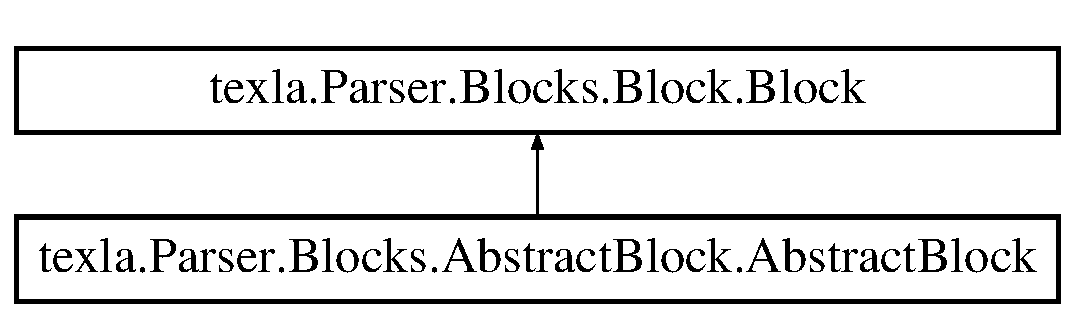
\includegraphics[height=2.000000cm]{classtexla_1_1Parser_1_1Blocks_1_1AbstractBlock_1_1AbstractBlock}
\end{center}
\end{figure}
\subsection*{Public Member Functions}
\begin{DoxyCompactItemize}
\item 
\hypertarget{classtexla_1_1Parser_1_1Blocks_1_1AbstractBlock_1_1AbstractBlock_ad247f4c7b6221e8a7d4084aa8ce43581}{}\label{classtexla_1_1Parser_1_1Blocks_1_1AbstractBlock_1_1AbstractBlock_ad247f4c7b6221e8a7d4084aa8ce43581} 
def {\bfseries \+\_\+\+\_\+init\+\_\+\+\_\+} (self, tex, parent\+\_\+block)
\end{DoxyCompactItemize}
\subsection*{Static Public Member Functions}
\begin{DoxyCompactItemize}
\item 
\hypertarget{classtexla_1_1Parser_1_1Blocks_1_1AbstractBlock_1_1AbstractBlock_ad4ad069cc2f0446f186fb852fec3a250}{}\label{classtexla_1_1Parser_1_1Blocks_1_1AbstractBlock_1_1AbstractBlock_ad4ad069cc2f0446f186fb852fec3a250} 
def {\bfseries parse} (parser, tex, parent\+\_\+block, params)
\end{DoxyCompactItemize}
\subsection*{Additional Inherited Members}


\subsection{Detailed Description}
\begin{DoxyVerb}This class handles the abstract environment\end{DoxyVerb}
 

The documentation for this class was generated from the following file\+:\begin{DoxyCompactItemize}
\item 
texla/\+Parser/\+Blocks/Abstract\+Block.\+py\end{DoxyCompactItemize}

\hypertarget{classtexla_1_1Parser_1_1Blocks_1_1TextBlocks_1_1AccentedLetterBlock}{}\section{texla.\+Parser.\+Blocks.\+Text\+Blocks.\+Accented\+Letter\+Block Class Reference}
\label{classtexla_1_1Parser_1_1Blocks_1_1TextBlocks_1_1AccentedLetterBlock}\index{texla.\+Parser.\+Blocks.\+Text\+Blocks.\+Accented\+Letter\+Block@{texla.\+Parser.\+Blocks.\+Text\+Blocks.\+Accented\+Letter\+Block}}
Inheritance diagram for texla.\+Parser.\+Blocks.\+Text\+Blocks.\+Accented\+Letter\+Block\+:\begin{figure}[H]
\begin{center}
\leavevmode
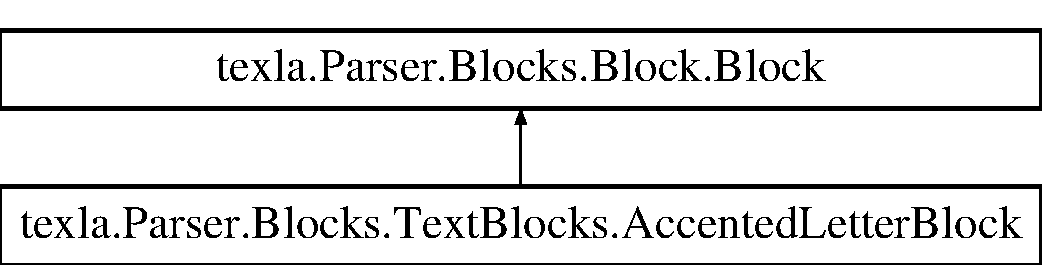
\includegraphics[height=2.000000cm]{classtexla_1_1Parser_1_1Blocks_1_1TextBlocks_1_1AccentedLetterBlock}
\end{center}
\end{figure}
\subsection*{Public Member Functions}
\begin{DoxyCompactItemize}
\item 
\hypertarget{classtexla_1_1Parser_1_1Blocks_1_1TextBlocks_1_1AccentedLetterBlock_a197fa3c5d1d8a6b1b75b82fce61149ab}{}\label{classtexla_1_1Parser_1_1Blocks_1_1TextBlocks_1_1AccentedLetterBlock_a197fa3c5d1d8a6b1b75b82fce61149ab} 
def {\bfseries \+\_\+\+\_\+init\+\_\+\+\_\+} (self, letter, accent\+\_\+type, parent\+\_\+block)
\item 
\hypertarget{classtexla_1_1Parser_1_1Blocks_1_1TextBlocks_1_1AccentedLetterBlock_af185fc3c8e3205e1eac1b3b9dcddb34f}{}\label{classtexla_1_1Parser_1_1Blocks_1_1TextBlocks_1_1AccentedLetterBlock_af185fc3c8e3205e1eac1b3b9dcddb34f} 
def {\bfseries \+\_\+\+\_\+str\+\_\+\+\_\+} (self)
\end{DoxyCompactItemize}
\subsection*{Static Public Member Functions}
\begin{DoxyCompactItemize}
\item 
\hypertarget{classtexla_1_1Parser_1_1Blocks_1_1TextBlocks_1_1AccentedLetterBlock_a60f0dd1d6b63dc79a24a284c60443833}{}\label{classtexla_1_1Parser_1_1Blocks_1_1TextBlocks_1_1AccentedLetterBlock_a60f0dd1d6b63dc79a24a284c60443833} 
def {\bfseries parse\+\_\+accents} (parser, tex, parent\+\_\+block, params)
\end{DoxyCompactItemize}
\subsection*{Additional Inherited Members}


The documentation for this class was generated from the following file\+:\begin{DoxyCompactItemize}
\item 
texla/\+Parser/\+Blocks/Text\+Blocks.\+py\end{DoxyCompactItemize}

\hypertarget{classtexla_1_1Parser_1_1Blocks_1_1AlignmentBlocks_1_1AlignmentBlock}{}\section{texla.\+Parser.\+Blocks.\+Alignment\+Blocks.\+Alignment\+Block Class Reference}
\label{classtexla_1_1Parser_1_1Blocks_1_1AlignmentBlocks_1_1AlignmentBlock}\index{texla.\+Parser.\+Blocks.\+Alignment\+Blocks.\+Alignment\+Block@{texla.\+Parser.\+Blocks.\+Alignment\+Blocks.\+Alignment\+Block}}
Inheritance diagram for texla.\+Parser.\+Blocks.\+Alignment\+Blocks.\+Alignment\+Block\+:\begin{figure}[H]
\begin{center}
\leavevmode
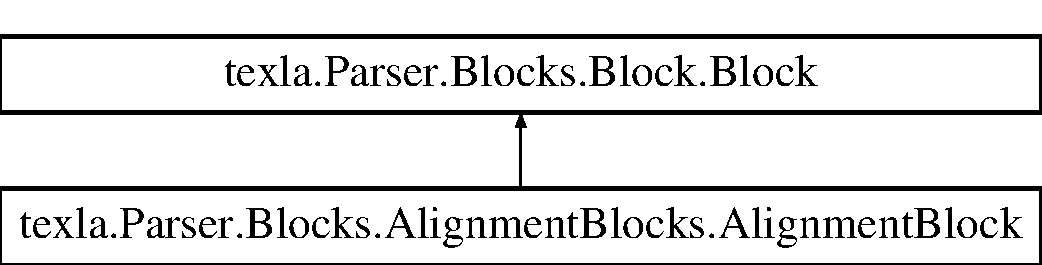
\includegraphics[height=2.000000cm]{classtexla_1_1Parser_1_1Blocks_1_1AlignmentBlocks_1_1AlignmentBlock}
\end{center}
\end{figure}
\subsection*{Public Member Functions}
\begin{DoxyCompactItemize}
\item 
\hypertarget{classtexla_1_1Parser_1_1Blocks_1_1AlignmentBlocks_1_1AlignmentBlock_a10f5e4db0a946b1ae6abe1f5285a12ac}{}\label{classtexla_1_1Parser_1_1Blocks_1_1AlignmentBlocks_1_1AlignmentBlock_a10f5e4db0a946b1ae6abe1f5285a12ac} 
def {\bfseries \+\_\+\+\_\+init\+\_\+\+\_\+} (self, align\+\_\+type, tex, parent\+\_\+block)
\item 
\hypertarget{classtexla_1_1Parser_1_1Blocks_1_1AlignmentBlocks_1_1AlignmentBlock_a5bde355ba093770bfdc68287d4b35ac2}{}\label{classtexla_1_1Parser_1_1Blocks_1_1AlignmentBlocks_1_1AlignmentBlock_a5bde355ba093770bfdc68287d4b35ac2} 
def {\bfseries \+\_\+\+\_\+str\+\_\+\+\_\+} (self)
\end{DoxyCompactItemize}
\subsection*{Static Public Member Functions}
\begin{DoxyCompactItemize}
\item 
\hypertarget{classtexla_1_1Parser_1_1Blocks_1_1AlignmentBlocks_1_1AlignmentBlock_a5498e23e4f9025796f66e743c74aba7e}{}\label{classtexla_1_1Parser_1_1Blocks_1_1AlignmentBlocks_1_1AlignmentBlock_a5498e23e4f9025796f66e743c74aba7e} 
def {\bfseries parse\+\_\+env} (parser, tex, parent\+\_\+block, params)
\item 
\hypertarget{classtexla_1_1Parser_1_1Blocks_1_1AlignmentBlocks_1_1AlignmentBlock_ab3ef5a2ec98c91849e439c477741f2ec}{}\label{classtexla_1_1Parser_1_1Blocks_1_1AlignmentBlocks_1_1AlignmentBlock_ab3ef5a2ec98c91849e439c477741f2ec} 
def {\bfseries parse\+\_\+command} (parser, tex, parent\+\_\+block, params)
\item 
\hypertarget{classtexla_1_1Parser_1_1Blocks_1_1AlignmentBlocks_1_1AlignmentBlock_ae542ab763e7cb2cb277e55974cd9db5c}{}\label{classtexla_1_1Parser_1_1Blocks_1_1AlignmentBlocks_1_1AlignmentBlock_ae542ab763e7cb2cb277e55974cd9db5c} 
def {\bfseries parse\+\_\+command\+\_\+content} (parser, tex, parent\+\_\+block, params)
\end{DoxyCompactItemize}
\subsection*{Additional Inherited Members}


\subsection{Detailed Description}
\begin{DoxyVerb}This class handles the flushright, flushleft
and center environments\end{DoxyVerb}
 

The documentation for this class was generated from the following file\+:\begin{DoxyCompactItemize}
\item 
texla/\+Parser/\+Blocks/Alignment\+Blocks.\+py\end{DoxyCompactItemize}

\hypertarget{classtexla_1_1PageTree_1_1Babel_1_1Babel}{}\section{texla.\+Page\+Tree.\+Babel.\+Babel Class Reference}
\label{classtexla_1_1PageTree_1_1Babel_1_1Babel}\index{texla.\+Page\+Tree.\+Babel.\+Babel@{texla.\+Page\+Tree.\+Babel.\+Babel}}
\subsection*{Public Member Functions}
\begin{DoxyCompactItemize}
\item 
\hypertarget{classtexla_1_1PageTree_1_1Babel_1_1Babel_a4c6cf7487957f67b98f1a7d6520e86ba}{}\label{classtexla_1_1PageTree_1_1Babel_1_1Babel_a4c6cf7487957f67b98f1a7d6520e86ba} 
def {\bfseries \+\_\+\+\_\+init\+\_\+\+\_\+} (self)
\item 
def \hyperlink{classtexla_1_1PageTree_1_1Babel_1_1Babel_a60491a66c7f0bbd27cbcdb10447e2902}{add\+\_\+label} (self, label, anchor)
\item 
def \hyperlink{classtexla_1_1PageTree_1_1Babel_1_1Babel_a9fa3d1d8628ea14de175e506640bc160}{add\+\_\+reference} (self, label, ref)
\item 
def \hyperlink{classtexla_1_1PageTree_1_1Babel_1_1Babel_a0c75743fd9b66c057b5a27900ccb8e32}{move\+\_\+anchor} (self, oldanc, newanc)
\item 
def \hyperlink{classtexla_1_1PageTree_1_1Babel_1_1Babel_a1d4846dd94d6c4c272303703b7438f9e}{fix\+\_\+references} (self)
\end{DoxyCompactItemize}
\subsection*{Public Attributes}
\begin{DoxyCompactItemize}
\item 
\hypertarget{classtexla_1_1PageTree_1_1Babel_1_1Babel_aad0f2a6c8574722a11a5ce0a7dee78bd}{}\label{classtexla_1_1PageTree_1_1Babel_1_1Babel_aad0f2a6c8574722a11a5ce0a7dee78bd} 
{\bfseries refs}
\item 
\hypertarget{classtexla_1_1PageTree_1_1Babel_1_1Babel_ad817351db8cee0a76bf2ef622bb02152}{}\label{classtexla_1_1PageTree_1_1Babel_1_1Babel_ad817351db8cee0a76bf2ef622bb02152} 
{\bfseries anchors}
\end{DoxyCompactItemize}


\subsection{Member Function Documentation}
\hypertarget{classtexla_1_1PageTree_1_1Babel_1_1Babel_a60491a66c7f0bbd27cbcdb10447e2902}{}\label{classtexla_1_1PageTree_1_1Babel_1_1Babel_a60491a66c7f0bbd27cbcdb10447e2902} 
\index{texla\+::\+Page\+Tree\+::\+Babel\+::\+Babel@{texla\+::\+Page\+Tree\+::\+Babel\+::\+Babel}!add\+\_\+label@{add\+\_\+label}}
\index{add\+\_\+label@{add\+\_\+label}!texla\+::\+Page\+Tree\+::\+Babel\+::\+Babel@{texla\+::\+Page\+Tree\+::\+Babel\+::\+Babel}}
\subsubsection{\texorpdfstring{add\+\_\+label()}{add\_label()}}
{\footnotesize\ttfamily def texla.\+Page\+Tree.\+Babel.\+Babel.\+add\+\_\+label (\begin{DoxyParamCaption}\item[{}]{self,  }\item[{}]{label,  }\item[{}]{anchor }\end{DoxyParamCaption})}

\begin{DoxyVerb}This method adds a label and its anchor to the
babel. The label is unique but can be overwritten.
\end{DoxyVerb}
 \hypertarget{classtexla_1_1PageTree_1_1Babel_1_1Babel_a9fa3d1d8628ea14de175e506640bc160}{}\label{classtexla_1_1PageTree_1_1Babel_1_1Babel_a9fa3d1d8628ea14de175e506640bc160} 
\index{texla\+::\+Page\+Tree\+::\+Babel\+::\+Babel@{texla\+::\+Page\+Tree\+::\+Babel\+::\+Babel}!add\+\_\+reference@{add\+\_\+reference}}
\index{add\+\_\+reference@{add\+\_\+reference}!texla\+::\+Page\+Tree\+::\+Babel\+::\+Babel@{texla\+::\+Page\+Tree\+::\+Babel\+::\+Babel}}
\subsubsection{\texorpdfstring{add\+\_\+reference()}{add\_reference()}}
{\footnotesize\ttfamily def texla.\+Page\+Tree.\+Babel.\+Babel.\+add\+\_\+reference (\begin{DoxyParamCaption}\item[{}]{self,  }\item[{}]{label,  }\item[{}]{ref }\end{DoxyParamCaption})}

\begin{DoxyVerb}This method adds a reference to the label.
A reference is a page or in general an object
with .text properties. The babel will fix the reference
of the registered objects.
\end{DoxyVerb}
 \hypertarget{classtexla_1_1PageTree_1_1Babel_1_1Babel_a1d4846dd94d6c4c272303703b7438f9e}{}\label{classtexla_1_1PageTree_1_1Babel_1_1Babel_a1d4846dd94d6c4c272303703b7438f9e} 
\index{texla\+::\+Page\+Tree\+::\+Babel\+::\+Babel@{texla\+::\+Page\+Tree\+::\+Babel\+::\+Babel}!fix\+\_\+references@{fix\+\_\+references}}
\index{fix\+\_\+references@{fix\+\_\+references}!texla\+::\+Page\+Tree\+::\+Babel\+::\+Babel@{texla\+::\+Page\+Tree\+::\+Babel\+::\+Babel}}
\subsubsection{\texorpdfstring{fix\+\_\+references()}{fix\_references()}}
{\footnotesize\ttfamily def texla.\+Page\+Tree.\+Babel.\+Babel.\+fix\+\_\+references (\begin{DoxyParamCaption}\item[{}]{self }\end{DoxyParamCaption})}

\begin{DoxyVerb}This method will fix the reference in the objects saved under
self.refs. The text {{ref:label}} in the objects' .text properties
will be replaces by a url made of [url|title]. The url and the title
MUST be properties of the anchor saved.
\end{DoxyVerb}
 \hypertarget{classtexla_1_1PageTree_1_1Babel_1_1Babel_a0c75743fd9b66c057b5a27900ccb8e32}{}\label{classtexla_1_1PageTree_1_1Babel_1_1Babel_a0c75743fd9b66c057b5a27900ccb8e32} 
\index{texla\+::\+Page\+Tree\+::\+Babel\+::\+Babel@{texla\+::\+Page\+Tree\+::\+Babel\+::\+Babel}!move\+\_\+anchor@{move\+\_\+anchor}}
\index{move\+\_\+anchor@{move\+\_\+anchor}!texla\+::\+Page\+Tree\+::\+Babel\+::\+Babel@{texla\+::\+Page\+Tree\+::\+Babel\+::\+Babel}}
\subsubsection{\texorpdfstring{move\+\_\+anchor()}{move\_anchor()}}
{\footnotesize\ttfamily def texla.\+Page\+Tree.\+Babel.\+Babel.\+move\+\_\+anchor (\begin{DoxyParamCaption}\item[{}]{self,  }\item[{}]{oldanc,  }\item[{}]{newanc }\end{DoxyParamCaption})}

\begin{DoxyVerb}This function replace the references to oldanc with newanc,
both as anchor and ref. It is used mainly when a page is moved\end{DoxyVerb}
 

The documentation for this class was generated from the following file\+:\begin{DoxyCompactItemize}
\item 
texla/\+Page\+Tree/Babel.\+py\end{DoxyCompactItemize}

\hypertarget{classtexla_1_1Parser_1_1Blocks_1_1Block_1_1Block}{}\section{texla.\+Parser.\+Blocks.\+Block.\+Block Class Reference}
\label{classtexla_1_1Parser_1_1Blocks_1_1Block_1_1Block}\index{texla.\+Parser.\+Blocks.\+Block.\+Block@{texla.\+Parser.\+Blocks.\+Block.\+Block}}
Inheritance diagram for texla.\+Parser.\+Blocks.\+Block.\+Block\+:\begin{figure}[H]
\begin{center}
\leavevmode
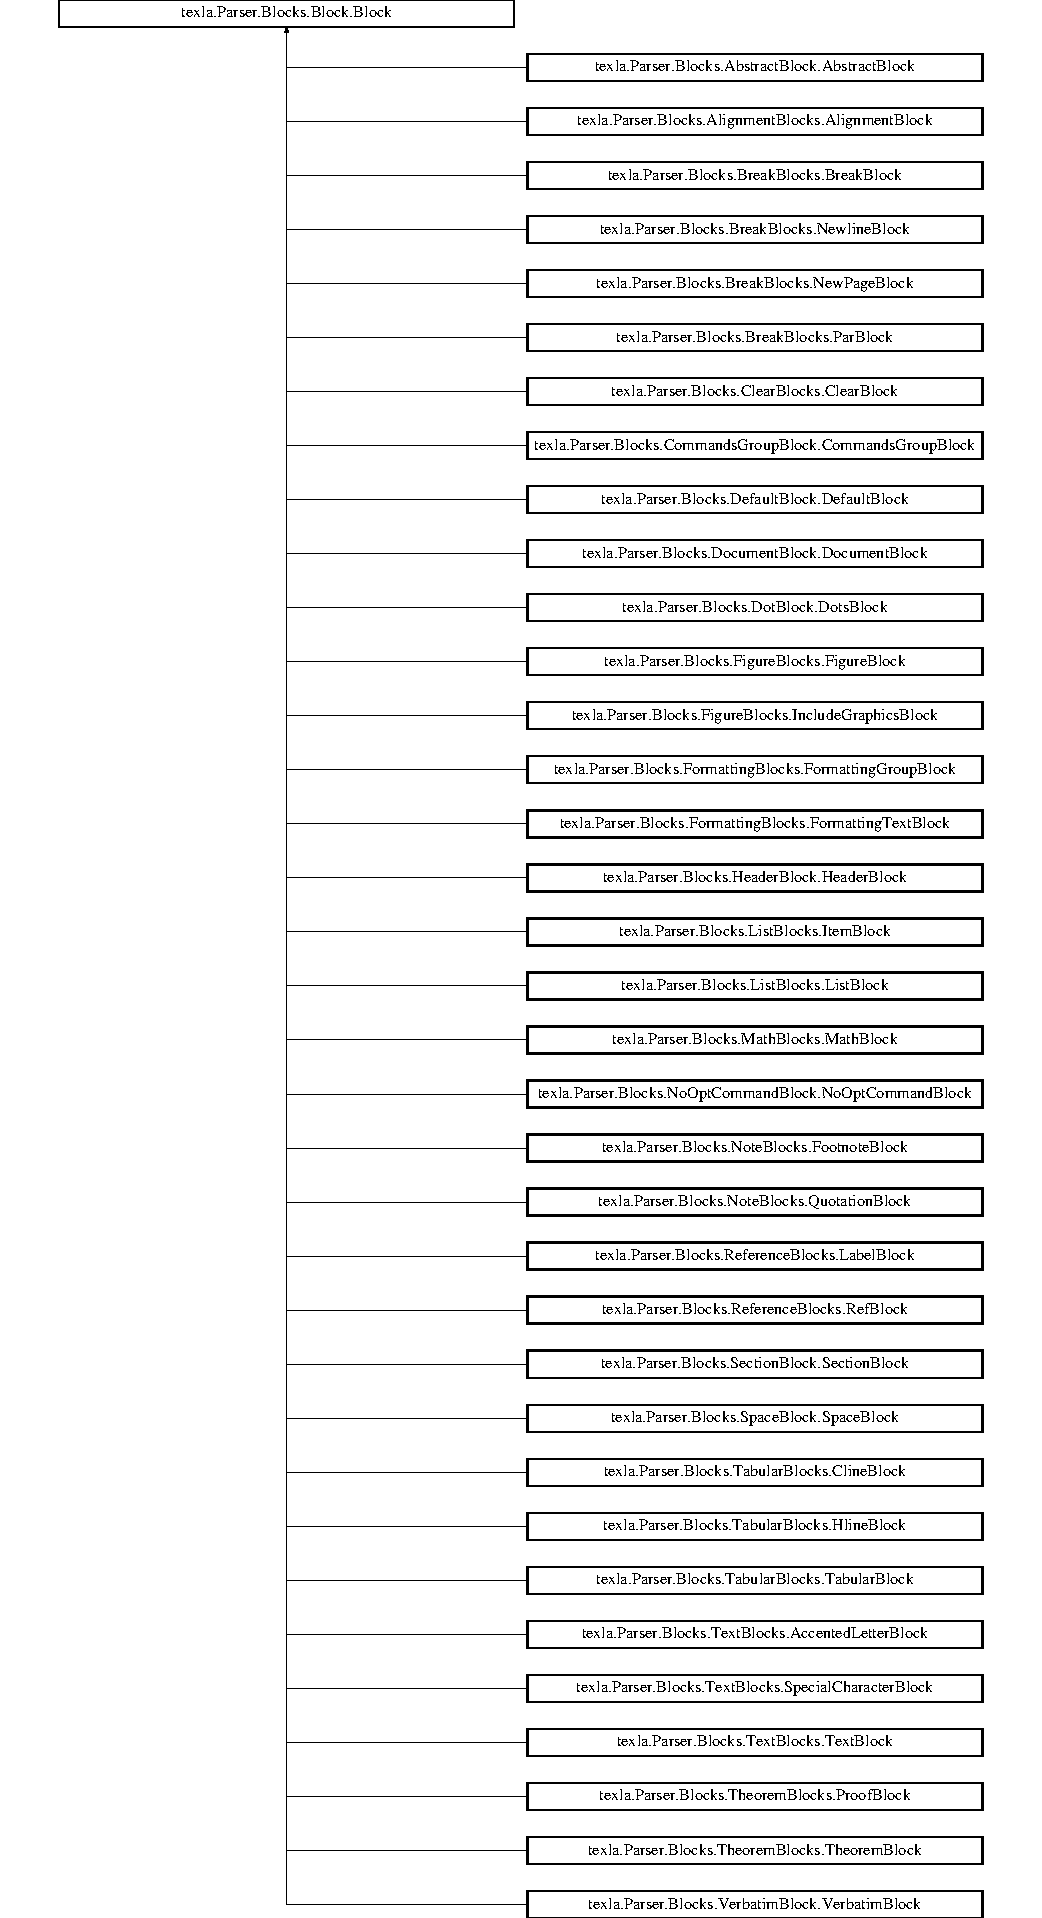
\includegraphics[height=12.000000cm]{classtexla_1_1Parser_1_1Blocks_1_1Block_1_1Block}
\end{center}
\end{figure}
\subsection*{Public Member Functions}
\begin{DoxyCompactItemize}
\item 
def \hyperlink{classtexla_1_1Parser_1_1Blocks_1_1Block_1_1Block_af80ceabfc4227532e63921f3d8387cfb}{\+\_\+\+\_\+init\+\_\+\+\_\+} (self, block\+\_\+name, content, parent\+\_\+block)
\item 
def \hyperlink{classtexla_1_1Parser_1_1Blocks_1_1Block_1_1Block_aba033196247b84b24bed702573350019}{add\+\_\+child\+\_\+block} (self, block)
\item 
def \hyperlink{classtexla_1_1Parser_1_1Blocks_1_1Block_1_1Block_a1529f89c563d66a4cde7cdbcc8e758de}{add\+\_\+children\+\_\+blocks} (self, blocks)
\item 
def \hyperlink{classtexla_1_1Parser_1_1Blocks_1_1Block_1_1Block_a5007c8a33e96707e02068ec65c30544a}{change\+\_\+parent\+\_\+block} (self, new\+\_\+parent)
\item 
\hypertarget{classtexla_1_1Parser_1_1Blocks_1_1Block_1_1Block_a6015fc7c8783c033f0abc81dedeb6695}{}\label{classtexla_1_1Parser_1_1Blocks_1_1Block_1_1Block_a6015fc7c8783c033f0abc81dedeb6695} 
def {\bfseries \+\_\+\+\_\+str\+\_\+\+\_\+} (self)
\item 
def \hyperlink{classtexla_1_1Parser_1_1Blocks_1_1Block_1_1Block_a80ef96fd4247bdaa6038eea0f5abf2cf}{to\+\_\+json} (self, level=0)
\item 
def \hyperlink{classtexla_1_1Parser_1_1Blocks_1_1Block_1_1Block_a5add9bf131b1916f0220363912d1baec}{n\+\_\+blocks} (self)
\end{DoxyCompactItemize}
\subsection*{Static Public Member Functions}
\begin{DoxyCompactItemize}
\item 
def \hyperlink{classtexla_1_1Parser_1_1Blocks_1_1Block_1_1Block_a2a2862dcf38b90cf8ad1bbd4e7c8f266}{parse} (parser, tex, parent\+\_\+block, params=\{\})
\end{DoxyCompactItemize}
\subsection*{Public Attributes}
\begin{DoxyCompactItemize}
\item 
\hypertarget{classtexla_1_1Parser_1_1Blocks_1_1Block_1_1Block_aaf91dadc0f7923f1b4a4db2acb4db553}{}\label{classtexla_1_1Parser_1_1Blocks_1_1Block_1_1Block_aaf91dadc0f7923f1b4a4db2acb4db553} 
{\bfseries block\+\_\+name}
\item 
\hypertarget{classtexla_1_1Parser_1_1Blocks_1_1Block_1_1Block_a7ae8475f8960c46daf6ee70732bdb011}{}\label{classtexla_1_1Parser_1_1Blocks_1_1Block_1_1Block_a7ae8475f8960c46daf6ee70732bdb011} 
{\bfseries content}
\item 
\hypertarget{classtexla_1_1Parser_1_1Blocks_1_1Block_1_1Block_aa2d6ad46fcdf734ef6c23eb5895a4b30}{}\label{classtexla_1_1Parser_1_1Blocks_1_1Block_1_1Block_aa2d6ad46fcdf734ef6c23eb5895a4b30} 
{\bfseries parent\+\_\+block}
\item 
\hypertarget{classtexla_1_1Parser_1_1Blocks_1_1Block_1_1Block_a1861a49a64fd1fb2942f6ff4ee555c90}{}\label{classtexla_1_1Parser_1_1Blocks_1_1Block_1_1Block_a1861a49a64fd1fb2942f6ff4ee555c90} 
{\bfseries id}
\item 
\hypertarget{classtexla_1_1Parser_1_1Blocks_1_1Block_1_1Block_a6c73db9ae118588c1c8c430121ec0501}{}\label{classtexla_1_1Parser_1_1Blocks_1_1Block_1_1Block_a6c73db9ae118588c1c8c430121ec0501} 
{\bfseries section\+\_\+level}
\item 
\hypertarget{classtexla_1_1Parser_1_1Blocks_1_1Block_1_1Block_a69e62063ec9a1b066dda624c16b970f1}{}\label{classtexla_1_1Parser_1_1Blocks_1_1Block_1_1Block_a69e62063ec9a1b066dda624c16b970f1} 
{\bfseries tree\+\_\+depth}
\item 
\hypertarget{classtexla_1_1Parser_1_1Blocks_1_1Block_1_1Block_ac356eba0dfe1efc0ebc2f2952952f79a}{}\label{classtexla_1_1Parser_1_1Blocks_1_1Block_1_1Block_ac356eba0dfe1efc0ebc2f2952952f79a} 
{\bfseries attributes}
\item 
\hypertarget{classtexla_1_1Parser_1_1Blocks_1_1Block_1_1Block_add374ab8833c5591f3bc1de55cd3e5b3}{}\label{classtexla_1_1Parser_1_1Blocks_1_1Block_1_1Block_add374ab8833c5591f3bc1de55cd3e5b3} 
{\bfseries ch\+\_\+blocks}
\item 
\hypertarget{classtexla_1_1Parser_1_1Blocks_1_1Block_1_1Block_a968dec374c61cd6773dd1aef2a04677e}{}\label{classtexla_1_1Parser_1_1Blocks_1_1Block_1_1Block_a968dec374c61cd6773dd1aef2a04677e} 
{\bfseries N\+\_\+chblocks}
\end{DoxyCompactItemize}


\subsection{Detailed Description}
\begin{DoxyVerb}Block general attributes:
-block_name: the new of the "type" of the block
-id: unique id for the block in the tree
-parent_block: parent in the tree
-attributes: a dictionary for description of the block.
    All useful parser data go into attributes
-ch_blocks: a list of children_blocks
-section_level: the position of the block compared to
    sectioning levels defined in utility.py

Derived Block could add more attributes.
\end{DoxyVerb}
 

\subsection{Constructor \& Destructor Documentation}
\hypertarget{classtexla_1_1Parser_1_1Blocks_1_1Block_1_1Block_af80ceabfc4227532e63921f3d8387cfb}{}\label{classtexla_1_1Parser_1_1Blocks_1_1Block_1_1Block_af80ceabfc4227532e63921f3d8387cfb} 
\index{texla\+::\+Parser\+::\+Blocks\+::\+Block\+::\+Block@{texla\+::\+Parser\+::\+Blocks\+::\+Block\+::\+Block}!\+\_\+\+\_\+init\+\_\+\+\_\+@{\+\_\+\+\_\+init\+\_\+\+\_\+}}
\index{\+\_\+\+\_\+init\+\_\+\+\_\+@{\+\_\+\+\_\+init\+\_\+\+\_\+}!texla\+::\+Parser\+::\+Blocks\+::\+Block\+::\+Block@{texla\+::\+Parser\+::\+Blocks\+::\+Block\+::\+Block}}
\subsubsection{\texorpdfstring{\+\_\+\+\_\+init\+\_\+\+\_\+()}{\_\_init\_\_()}}
{\footnotesize\ttfamily def texla.\+Parser.\+Blocks.\+Block.\+Block.\+\_\+\+\_\+init\+\_\+\+\_\+ (\begin{DoxyParamCaption}\item[{}]{self,  }\item[{}]{block\+\_\+name,  }\item[{}]{content,  }\item[{}]{parent\+\_\+block }\end{DoxyParamCaption})}

\begin{DoxyVerb}Base constructor for Block.
It saves the parent_block and block name and create
the new id for the new block. It creates data structures
like the attributed dictionary and children nodes list.
It always saves a content variable.
By default, it sets the section_level of the block
to that of the parend_block.
\end{DoxyVerb}
 

\subsection{Member Function Documentation}
\hypertarget{classtexla_1_1Parser_1_1Blocks_1_1Block_1_1Block_aba033196247b84b24bed702573350019}{}\label{classtexla_1_1Parser_1_1Blocks_1_1Block_1_1Block_aba033196247b84b24bed702573350019} 
\index{texla\+::\+Parser\+::\+Blocks\+::\+Block\+::\+Block@{texla\+::\+Parser\+::\+Blocks\+::\+Block\+::\+Block}!add\+\_\+child\+\_\+block@{add\+\_\+child\+\_\+block}}
\index{add\+\_\+child\+\_\+block@{add\+\_\+child\+\_\+block}!texla\+::\+Parser\+::\+Blocks\+::\+Block\+::\+Block@{texla\+::\+Parser\+::\+Blocks\+::\+Block\+::\+Block}}
\subsubsection{\texorpdfstring{add\+\_\+child\+\_\+block()}{add\_child\_block()}}
{\footnotesize\ttfamily def texla.\+Parser.\+Blocks.\+Block.\+Block.\+add\+\_\+child\+\_\+block (\begin{DoxyParamCaption}\item[{}]{self,  }\item[{}]{block }\end{DoxyParamCaption})}

\begin{DoxyVerb}IMPORTANT: this function is called by the self.parse fuction.
It MUST NOT be called from outside, expecially the parser
\end{DoxyVerb}
 \hypertarget{classtexla_1_1Parser_1_1Blocks_1_1Block_1_1Block_a1529f89c563d66a4cde7cdbcc8e758de}{}\label{classtexla_1_1Parser_1_1Blocks_1_1Block_1_1Block_a1529f89c563d66a4cde7cdbcc8e758de} 
\index{texla\+::\+Parser\+::\+Blocks\+::\+Block\+::\+Block@{texla\+::\+Parser\+::\+Blocks\+::\+Block\+::\+Block}!add\+\_\+children\+\_\+blocks@{add\+\_\+children\+\_\+blocks}}
\index{add\+\_\+children\+\_\+blocks@{add\+\_\+children\+\_\+blocks}!texla\+::\+Parser\+::\+Blocks\+::\+Block\+::\+Block@{texla\+::\+Parser\+::\+Blocks\+::\+Block\+::\+Block}}
\subsubsection{\texorpdfstring{add\+\_\+children\+\_\+blocks()}{add\_children\_blocks()}}
{\footnotesize\ttfamily def texla.\+Parser.\+Blocks.\+Block.\+Block.\+add\+\_\+children\+\_\+blocks (\begin{DoxyParamCaption}\item[{}]{self,  }\item[{}]{blocks }\end{DoxyParamCaption})}

\begin{DoxyVerb}IMPORTANT: this function is called by the self.parse fuction.
It MUST NOT be called from outside, expecially the parser
\end{DoxyVerb}
 \hypertarget{classtexla_1_1Parser_1_1Blocks_1_1Block_1_1Block_a5007c8a33e96707e02068ec65c30544a}{}\label{classtexla_1_1Parser_1_1Blocks_1_1Block_1_1Block_a5007c8a33e96707e02068ec65c30544a} 
\index{texla\+::\+Parser\+::\+Blocks\+::\+Block\+::\+Block@{texla\+::\+Parser\+::\+Blocks\+::\+Block\+::\+Block}!change\+\_\+parent\+\_\+block@{change\+\_\+parent\+\_\+block}}
\index{change\+\_\+parent\+\_\+block@{change\+\_\+parent\+\_\+block}!texla\+::\+Parser\+::\+Blocks\+::\+Block\+::\+Block@{texla\+::\+Parser\+::\+Blocks\+::\+Block\+::\+Block}}
\subsubsection{\texorpdfstring{change\+\_\+parent\+\_\+block()}{change\_parent\_block()}}
{\footnotesize\ttfamily def texla.\+Parser.\+Blocks.\+Block.\+Block.\+change\+\_\+parent\+\_\+block (\begin{DoxyParamCaption}\item[{}]{self,  }\item[{}]{new\+\_\+parent }\end{DoxyParamCaption})}

\begin{DoxyVerb}This function changes the parent of the
block. It changes parent object, id, and tree_depth.
The section level is not changes for consistency.
All children are updated.
\end{DoxyVerb}
 \hypertarget{classtexla_1_1Parser_1_1Blocks_1_1Block_1_1Block_a5add9bf131b1916f0220363912d1baec}{}\label{classtexla_1_1Parser_1_1Blocks_1_1Block_1_1Block_a5add9bf131b1916f0220363912d1baec} 
\index{texla\+::\+Parser\+::\+Blocks\+::\+Block\+::\+Block@{texla\+::\+Parser\+::\+Blocks\+::\+Block\+::\+Block}!n\+\_\+blocks@{n\+\_\+blocks}}
\index{n\+\_\+blocks@{n\+\_\+blocks}!texla\+::\+Parser\+::\+Blocks\+::\+Block\+::\+Block@{texla\+::\+Parser\+::\+Blocks\+::\+Block\+::\+Block}}
\subsubsection{\texorpdfstring{n\+\_\+blocks()}{n\_blocks()}}
{\footnotesize\ttfamily def texla.\+Parser.\+Blocks.\+Block.\+Block.\+n\+\_\+blocks (\begin{DoxyParamCaption}\item[{}]{self }\end{DoxyParamCaption})}

\begin{DoxyVerb}This function returns the
number of all children blocks recursively.\end{DoxyVerb}
 \hypertarget{classtexla_1_1Parser_1_1Blocks_1_1Block_1_1Block_a2a2862dcf38b90cf8ad1bbd4e7c8f266}{}\label{classtexla_1_1Parser_1_1Blocks_1_1Block_1_1Block_a2a2862dcf38b90cf8ad1bbd4e7c8f266} 
\index{texla\+::\+Parser\+::\+Blocks\+::\+Block\+::\+Block@{texla\+::\+Parser\+::\+Blocks\+::\+Block\+::\+Block}!parse@{parse}}
\index{parse@{parse}!texla\+::\+Parser\+::\+Blocks\+::\+Block\+::\+Block@{texla\+::\+Parser\+::\+Blocks\+::\+Block\+::\+Block}}
\subsubsection{\texorpdfstring{parse()}{parse()}}
{\footnotesize\ttfamily def texla.\+Parser.\+Blocks.\+Block.\+Block.\+parse (\begin{DoxyParamCaption}\item[{}]{parser,  }\item[{}]{tex,  }\item[{}]{parent\+\_\+block,  }\item[{}]{params = {\ttfamily \{\}} }\end{DoxyParamCaption})\hspace{0.3cm}{\ttfamily [static]}}

\begin{DoxyVerb}The method must return a tuple with the created
Block and the last used index of tex string.\end{DoxyVerb}
 \hypertarget{classtexla_1_1Parser_1_1Blocks_1_1Block_1_1Block_a80ef96fd4247bdaa6038eea0f5abf2cf}{}\label{classtexla_1_1Parser_1_1Blocks_1_1Block_1_1Block_a80ef96fd4247bdaa6038eea0f5abf2cf} 
\index{texla\+::\+Parser\+::\+Blocks\+::\+Block\+::\+Block@{texla\+::\+Parser\+::\+Blocks\+::\+Block\+::\+Block}!to\+\_\+json@{to\+\_\+json}}
\index{to\+\_\+json@{to\+\_\+json}!texla\+::\+Parser\+::\+Blocks\+::\+Block\+::\+Block@{texla\+::\+Parser\+::\+Blocks\+::\+Block\+::\+Block}}
\subsubsection{\texorpdfstring{to\+\_\+json()}{to\_json()}}
{\footnotesize\ttfamily def texla.\+Parser.\+Blocks.\+Block.\+Block.\+to\+\_\+json (\begin{DoxyParamCaption}\item[{}]{self,  }\item[{}]{level = {\ttfamily 0} }\end{DoxyParamCaption})}

\begin{DoxyVerb}This functions create a json ouput that
represents the tree of subblocks of the called block.
\end{DoxyVerb}
 

The documentation for this class was generated from the following file\+:\begin{DoxyCompactItemize}
\item 
texla/\+Parser/\+Blocks/Block.\+py\end{DoxyCompactItemize}

\hypertarget{classtexla_1_1Parser_1_1Blocks_1_1BreakBlocks_1_1BreakBlock}{}\section{texla.\+Parser.\+Blocks.\+Break\+Blocks.\+Break\+Block Class Reference}
\label{classtexla_1_1Parser_1_1Blocks_1_1BreakBlocks_1_1BreakBlock}\index{texla.\+Parser.\+Blocks.\+Break\+Blocks.\+Break\+Block@{texla.\+Parser.\+Blocks.\+Break\+Blocks.\+Break\+Block}}
Inheritance diagram for texla.\+Parser.\+Blocks.\+Break\+Blocks.\+Break\+Block\+:\begin{figure}[H]
\begin{center}
\leavevmode
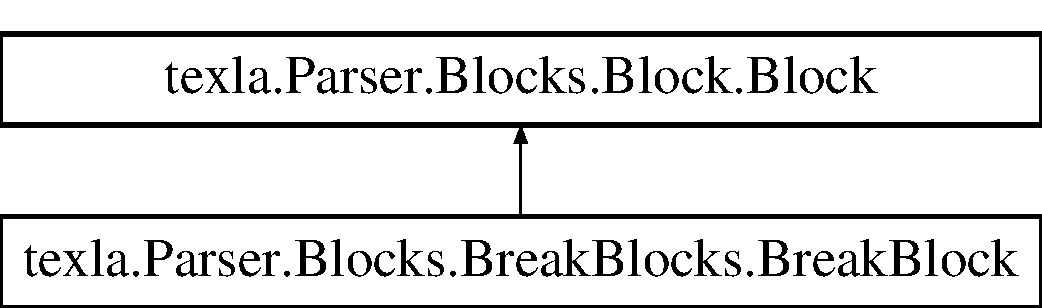
\includegraphics[height=2.000000cm]{classtexla_1_1Parser_1_1Blocks_1_1BreakBlocks_1_1BreakBlock}
\end{center}
\end{figure}
\subsection*{Public Member Functions}
\begin{DoxyCompactItemize}
\item 
\hypertarget{classtexla_1_1Parser_1_1Blocks_1_1BreakBlocks_1_1BreakBlock_a6344aaa52b1730c58f68e35e090d3452}{}\label{classtexla_1_1Parser_1_1Blocks_1_1BreakBlocks_1_1BreakBlock_a6344aaa52b1730c58f68e35e090d3452} 
def {\bfseries \+\_\+\+\_\+init\+\_\+\+\_\+} (self, break\+\_\+type, priority, content, parent\+\_\+block)
\end{DoxyCompactItemize}
\subsection*{Static Public Member Functions}
\begin{DoxyCompactItemize}
\item 
\hypertarget{classtexla_1_1Parser_1_1Blocks_1_1BreakBlocks_1_1BreakBlock_ad1ae2ce55d93242cf3a6ebdee687eb34}{}\label{classtexla_1_1Parser_1_1Blocks_1_1BreakBlocks_1_1BreakBlock_ad1ae2ce55d93242cf3a6ebdee687eb34} 
def {\bfseries parse} (parser, tex, parent\+\_\+block, params)
\end{DoxyCompactItemize}
\subsection*{Additional Inherited Members}


\subsection{Detailed Description}
\begin{DoxyVerb}This class gives you the possibility to
    break/not break a line/page\end{DoxyVerb}
 

The documentation for this class was generated from the following file\+:\begin{DoxyCompactItemize}
\item 
texla/\+Parser/\+Blocks/Break\+Blocks.\+py\end{DoxyCompactItemize}

\hypertarget{classtexla_1_1Parser_1_1Blocks_1_1ClearBlocks_1_1ClearBlock}{}\section{texla.\+Parser.\+Blocks.\+Clear\+Blocks.\+Clear\+Block Class Reference}
\label{classtexla_1_1Parser_1_1Blocks_1_1ClearBlocks_1_1ClearBlock}\index{texla.\+Parser.\+Blocks.\+Clear\+Blocks.\+Clear\+Block@{texla.\+Parser.\+Blocks.\+Clear\+Blocks.\+Clear\+Block}}
Inheritance diagram for texla.\+Parser.\+Blocks.\+Clear\+Blocks.\+Clear\+Block\+:\begin{figure}[H]
\begin{center}
\leavevmode
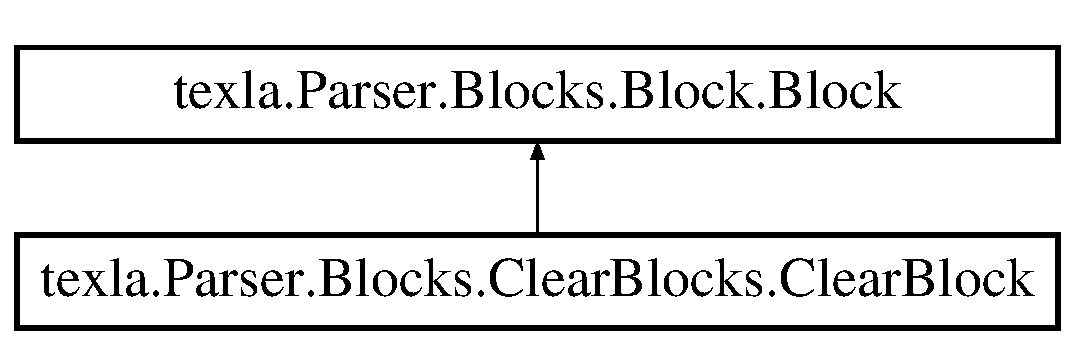
\includegraphics[height=2.000000cm]{classtexla_1_1Parser_1_1Blocks_1_1ClearBlocks_1_1ClearBlock}
\end{center}
\end{figure}
\subsection*{Public Member Functions}
\begin{DoxyCompactItemize}
\item 
\hypertarget{classtexla_1_1Parser_1_1Blocks_1_1ClearBlocks_1_1ClearBlock_aafb0db30c7bc1cf1990289269edd8935}{}\label{classtexla_1_1Parser_1_1Blocks_1_1ClearBlocks_1_1ClearBlock_aafb0db30c7bc1cf1990289269edd8935} 
def {\bfseries \+\_\+\+\_\+init\+\_\+\+\_\+} (self, clear\+\_\+type, parent\+\_\+block)
\end{DoxyCompactItemize}
\subsection*{Static Public Member Functions}
\begin{DoxyCompactItemize}
\item 
\hypertarget{classtexla_1_1Parser_1_1Blocks_1_1ClearBlocks_1_1ClearBlock_a86bc4796a454ddc54a65ae9b128de284}{}\label{classtexla_1_1Parser_1_1Blocks_1_1ClearBlocks_1_1ClearBlock_a86bc4796a454ddc54a65ae9b128de284} 
def {\bfseries parse} (parser, tex, parent\+\_\+block, params)
\end{DoxyCompactItemize}
\subsection*{Additional Inherited Members}


\subsection{Detailed Description}
\begin{DoxyVerb}Block that  ends the current page
and causes all figures and tables that
have so far appeared in the input to be printed\end{DoxyVerb}
 

The documentation for this class was generated from the following file\+:\begin{DoxyCompactItemize}
\item 
texla/\+Parser/\+Blocks/Clear\+Blocks.\+py\end{DoxyCompactItemize}

\hypertarget{classtexla_1_1Parser_1_1Blocks_1_1TabularBlocks_1_1ClineBlock}{}\section{texla.\+Parser.\+Blocks.\+Tabular\+Blocks.\+Cline\+Block Class Reference}
\label{classtexla_1_1Parser_1_1Blocks_1_1TabularBlocks_1_1ClineBlock}\index{texla.\+Parser.\+Blocks.\+Tabular\+Blocks.\+Cline\+Block@{texla.\+Parser.\+Blocks.\+Tabular\+Blocks.\+Cline\+Block}}
Inheritance diagram for texla.\+Parser.\+Blocks.\+Tabular\+Blocks.\+Cline\+Block\+:\begin{figure}[H]
\begin{center}
\leavevmode
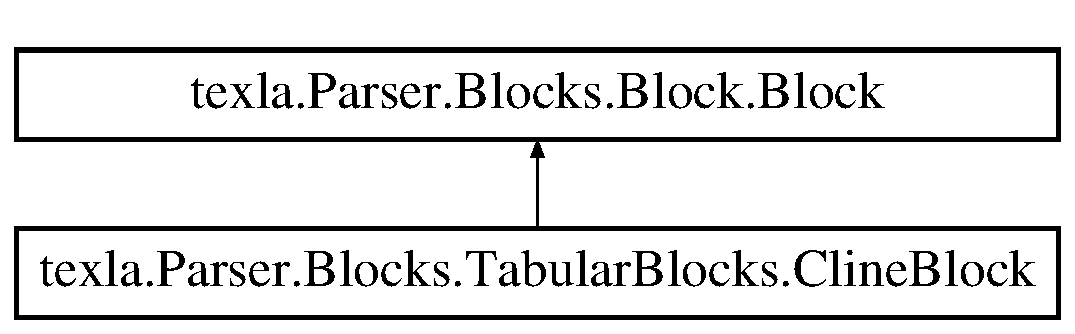
\includegraphics[height=2.000000cm]{classtexla_1_1Parser_1_1Blocks_1_1TabularBlocks_1_1ClineBlock}
\end{center}
\end{figure}
\subsection*{Public Member Functions}
\begin{DoxyCompactItemize}
\item 
\hypertarget{classtexla_1_1Parser_1_1Blocks_1_1TabularBlocks_1_1ClineBlock_aaefc14803bed8851a50098c108c7f982}{}\label{classtexla_1_1Parser_1_1Blocks_1_1TabularBlocks_1_1ClineBlock_aaefc14803bed8851a50098c108c7f982} 
def {\bfseries \+\_\+\+\_\+init\+\_\+\+\_\+} (self, start, end, parent\+\_\+block)
\end{DoxyCompactItemize}
\subsection*{Static Public Member Functions}
\begin{DoxyCompactItemize}
\item 
\hypertarget{classtexla_1_1Parser_1_1Blocks_1_1TabularBlocks_1_1ClineBlock_a7c5c86e1e06bfcb424579f42fb8e65eb}{}\label{classtexla_1_1Parser_1_1Blocks_1_1TabularBlocks_1_1ClineBlock_a7c5c86e1e06bfcb424579f42fb8e65eb} 
def {\bfseries parse} (parser, tex, parent\+\_\+block, params)
\end{DoxyCompactItemize}
\subsection*{Additional Inherited Members}


The documentation for this class was generated from the following file\+:\begin{DoxyCompactItemize}
\item 
texla/\+Parser/\+Blocks/Tabular\+Blocks.\+py\end{DoxyCompactItemize}

\hypertarget{classtexla_1_1Parser_1_1Blocks_1_1CommandsGroupBlock_1_1CommandsGroupBlock}{}\section{texla.\+Parser.\+Blocks.\+Commands\+Group\+Block.\+Commands\+Group\+Block Class Reference}
\label{classtexla_1_1Parser_1_1Blocks_1_1CommandsGroupBlock_1_1CommandsGroupBlock}\index{texla.\+Parser.\+Blocks.\+Commands\+Group\+Block.\+Commands\+Group\+Block@{texla.\+Parser.\+Blocks.\+Commands\+Group\+Block.\+Commands\+Group\+Block}}
Inheritance diagram for texla.\+Parser.\+Blocks.\+Commands\+Group\+Block.\+Commands\+Group\+Block\+:\begin{figure}[H]
\begin{center}
\leavevmode
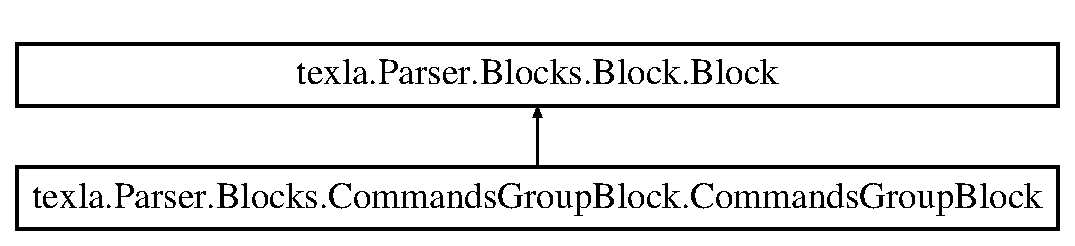
\includegraphics[height=2.000000cm]{classtexla_1_1Parser_1_1Blocks_1_1CommandsGroupBlock_1_1CommandsGroupBlock}
\end{center}
\end{figure}
\subsection*{Public Member Functions}
\begin{DoxyCompactItemize}
\item 
\hypertarget{classtexla_1_1Parser_1_1Blocks_1_1CommandsGroupBlock_1_1CommandsGroupBlock_ac7053bdfedcb59b925296b9b35f22792}{}\label{classtexla_1_1Parser_1_1Blocks_1_1CommandsGroupBlock_1_1CommandsGroupBlock_ac7053bdfedcb59b925296b9b35f22792} 
def {\bfseries \+\_\+\+\_\+init\+\_\+\+\_\+} (self, content, parent\+\_\+block)
\end{DoxyCompactItemize}
\subsection*{Static Public Member Functions}
\begin{DoxyCompactItemize}
\item 
\hypertarget{classtexla_1_1Parser_1_1Blocks_1_1CommandsGroupBlock_1_1CommandsGroupBlock_ac363b42da3c96959006dcc9d9ad9f885}{}\label{classtexla_1_1Parser_1_1Blocks_1_1CommandsGroupBlock_1_1CommandsGroupBlock_ac363b42da3c96959006dcc9d9ad9f885} 
def {\bfseries parse} (parser, tex, parent\+\_\+block, params)
\end{DoxyCompactItemize}
\subsection*{Public Attributes}
\begin{DoxyCompactItemize}
\item 
\hypertarget{classtexla_1_1Parser_1_1Blocks_1_1CommandsGroupBlock_1_1CommandsGroupBlock_a59010e7a5f58f96a12cb32b843271313}{}\label{classtexla_1_1Parser_1_1Blocks_1_1CommandsGroupBlock_1_1CommandsGroupBlock_a59010e7a5f58f96a12cb32b843271313} 
{\bfseries formatting}
\end{DoxyCompactItemize}


\subsection{Detailed Description}
\begin{DoxyVerb}This block represents the syntax {...}.
It is used to group formatting commands.
These commands are parsed normally in FormattingBlocks.py
and then catched by this block analyzing the ch_blocks.
Formatting commands are saved inside formatting list
as FormattingGroupBlock objects, ready for rendering.
\end{DoxyVerb}
 

The documentation for this class was generated from the following file\+:\begin{DoxyCompactItemize}
\item 
texla/\+Parser/\+Blocks/Commands\+Group\+Block.\+py\end{DoxyCompactItemize}

\hypertarget{classtexla_1_1Parser_1_1Blocks_1_1DefaultBlock_1_1DefaultBlock}{}\section{texla.\+Parser.\+Blocks.\+Default\+Block.\+Default\+Block Class Reference}
\label{classtexla_1_1Parser_1_1Blocks_1_1DefaultBlock_1_1DefaultBlock}\index{texla.\+Parser.\+Blocks.\+Default\+Block.\+Default\+Block@{texla.\+Parser.\+Blocks.\+Default\+Block.\+Default\+Block}}
Inheritance diagram for texla.\+Parser.\+Blocks.\+Default\+Block.\+Default\+Block\+:\begin{figure}[H]
\begin{center}
\leavevmode
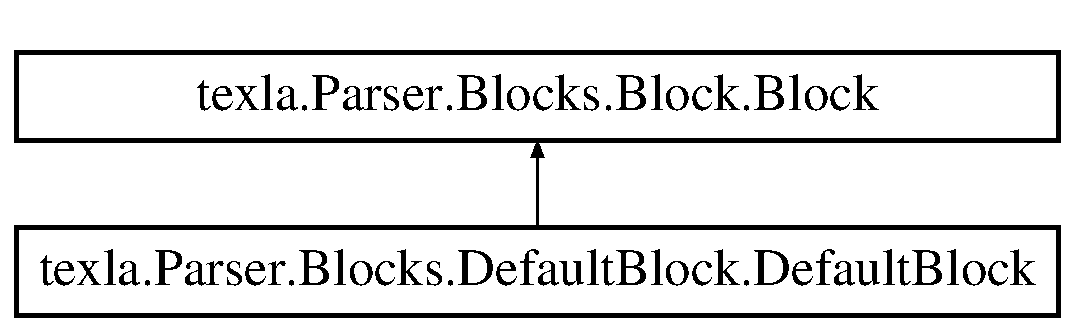
\includegraphics[height=2.000000cm]{classtexla_1_1Parser_1_1Blocks_1_1DefaultBlock_1_1DefaultBlock}
\end{center}
\end{figure}
\subsection*{Public Member Functions}
\begin{DoxyCompactItemize}
\item 
def \hyperlink{classtexla_1_1Parser_1_1Blocks_1_1DefaultBlock_1_1DefaultBlock_a4425df7cb1f458672c3e733f982f4cd5}{\+\_\+\+\_\+init\+\_\+\+\_\+} (self, tex, block\+\_\+name, parent\+\_\+block)
\end{DoxyCompactItemize}
\subsection*{Static Public Member Functions}
\begin{DoxyCompactItemize}
\item 
\hypertarget{classtexla_1_1Parser_1_1Blocks_1_1DefaultBlock_1_1DefaultBlock_adafd8b34760a28e49bb110fd1ffc110c}{}\label{classtexla_1_1Parser_1_1Blocks_1_1DefaultBlock_1_1DefaultBlock_adafd8b34760a28e49bb110fd1ffc110c} 
def {\bfseries parse\+\_\+env} (parser, tex, parent\+\_\+block, params)
\item 
\hypertarget{classtexla_1_1Parser_1_1Blocks_1_1DefaultBlock_1_1DefaultBlock_a27009494f899a4d6b488ba39a2dd830c}{}\label{classtexla_1_1Parser_1_1Blocks_1_1DefaultBlock_1_1DefaultBlock_a27009494f899a4d6b488ba39a2dd830c} 
def {\bfseries parse\+\_\+cmd} (parser, tex, parent\+\_\+block, params)
\end{DoxyCompactItemize}
\subsection*{Additional Inherited Members}


\subsection{Detailed Description}
\begin{DoxyVerb}This Block is used when the parser doesn't find
a proper parser_hook to call for a matched env or command\end{DoxyVerb}
 

\subsection{Constructor \& Destructor Documentation}
\hypertarget{classtexla_1_1Parser_1_1Blocks_1_1DefaultBlock_1_1DefaultBlock_a4425df7cb1f458672c3e733f982f4cd5}{}\label{classtexla_1_1Parser_1_1Blocks_1_1DefaultBlock_1_1DefaultBlock_a4425df7cb1f458672c3e733f982f4cd5} 
\index{texla\+::\+Parser\+::\+Blocks\+::\+Default\+Block\+::\+Default\+Block@{texla\+::\+Parser\+::\+Blocks\+::\+Default\+Block\+::\+Default\+Block}!\+\_\+\+\_\+init\+\_\+\+\_\+@{\+\_\+\+\_\+init\+\_\+\+\_\+}}
\index{\+\_\+\+\_\+init\+\_\+\+\_\+@{\+\_\+\+\_\+init\+\_\+\+\_\+}!texla\+::\+Parser\+::\+Blocks\+::\+Default\+Block\+::\+Default\+Block@{texla\+::\+Parser\+::\+Blocks\+::\+Default\+Block\+::\+Default\+Block}}
\subsubsection{\texorpdfstring{\+\_\+\+\_\+init\+\_\+\+\_\+()}{\_\_init\_\_()}}
{\footnotesize\ttfamily def texla.\+Parser.\+Blocks.\+Default\+Block.\+Default\+Block.\+\_\+\+\_\+init\+\_\+\+\_\+ (\begin{DoxyParamCaption}\item[{}]{self,  }\item[{}]{tex,  }\item[{}]{block\+\_\+name,  }\item[{}]{parent\+\_\+block }\end{DoxyParamCaption})}

\begin{DoxyVerb}Constructor for sections:
-title: main title
-index_title: title for table of content
-numbered: True/False
-level: sections level
-parent_block
\end{DoxyVerb}
 

The documentation for this class was generated from the following file\+:\begin{DoxyCompactItemize}
\item 
texla/\+Parser/\+Blocks/Default\+Block.\+py\end{DoxyCompactItemize}

\hypertarget{classtexla_1_1Parser_1_1Blocks_1_1DocumentBlock_1_1DocumentBlock}{}\section{texla.\+Parser.\+Blocks.\+Document\+Block.\+Document\+Block Class Reference}
\label{classtexla_1_1Parser_1_1Blocks_1_1DocumentBlock_1_1DocumentBlock}\index{texla.\+Parser.\+Blocks.\+Document\+Block.\+Document\+Block@{texla.\+Parser.\+Blocks.\+Document\+Block.\+Document\+Block}}
Inheritance diagram for texla.\+Parser.\+Blocks.\+Document\+Block.\+Document\+Block\+:\begin{figure}[H]
\begin{center}
\leavevmode
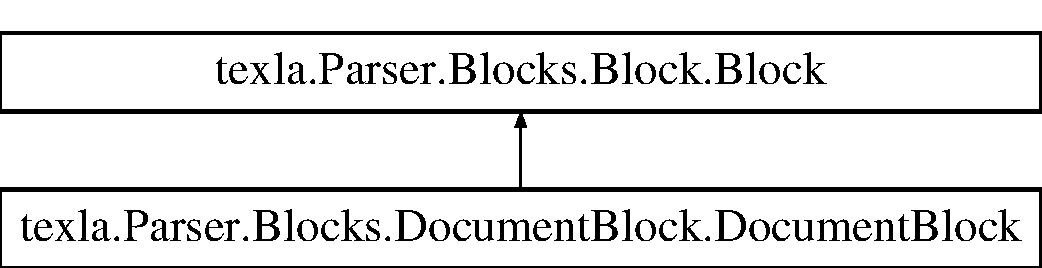
\includegraphics[height=2.000000cm]{classtexla_1_1Parser_1_1Blocks_1_1DocumentBlock_1_1DocumentBlock}
\end{center}
\end{figure}
\subsection*{Public Member Functions}
\begin{DoxyCompactItemize}
\item 
\hypertarget{classtexla_1_1Parser_1_1Blocks_1_1DocumentBlock_1_1DocumentBlock_a6bda8551b757a0f59387f8e1f61aec00}{}\label{classtexla_1_1Parser_1_1Blocks_1_1DocumentBlock_1_1DocumentBlock_a6bda8551b757a0f59387f8e1f61aec00} 
def {\bfseries \+\_\+\+\_\+init\+\_\+\+\_\+} (self, title, options)
\end{DoxyCompactItemize}
\subsection*{Public Attributes}
\begin{DoxyCompactItemize}
\item 
\hypertarget{classtexla_1_1Parser_1_1Blocks_1_1DocumentBlock_1_1DocumentBlock_a652fe5f9c1b3f599eddf758e12543a15}{}\label{classtexla_1_1Parser_1_1Blocks_1_1DocumentBlock_1_1DocumentBlock_a652fe5f9c1b3f599eddf758e12543a15} 
{\bfseries title}
\item 
\hypertarget{classtexla_1_1Parser_1_1Blocks_1_1DocumentBlock_1_1DocumentBlock_a3ef629c7fc2493d105d83f8a7074e0c0}{}\label{classtexla_1_1Parser_1_1Blocks_1_1DocumentBlock_1_1DocumentBlock_a3ef629c7fc2493d105d83f8a7074e0c0} 
{\bfseries options}
\item 
\hypertarget{classtexla_1_1Parser_1_1Blocks_1_1DocumentBlock_1_1DocumentBlock_a4e881a864dc372efca10e6af0e5b5f61}{}\label{classtexla_1_1Parser_1_1Blocks_1_1DocumentBlock_1_1DocumentBlock_a4e881a864dc372efca10e6af0e5b5f61} 
{\bfseries section\+\_\+level}
\item 
\hypertarget{classtexla_1_1Parser_1_1Blocks_1_1DocumentBlock_1_1DocumentBlock_a686b15909870fcd0b7c96ac8103de12e}{}\label{classtexla_1_1Parser_1_1Blocks_1_1DocumentBlock_1_1DocumentBlock_a686b15909870fcd0b7c96ac8103de12e} 
{\bfseries tree\+\_\+depth}
\end{DoxyCompactItemize}
\subsection*{Additional Inherited Members}


The documentation for this class was generated from the following file\+:\begin{DoxyCompactItemize}
\item 
texla/\+Parser/\+Blocks/Document\+Block.\+py\end{DoxyCompactItemize}

\hypertarget{classtexla_1_1Parser_1_1Blocks_1_1DotBlock_1_1DotsBlock}{}\section{texla.\+Parser.\+Blocks.\+Dot\+Block.\+Dots\+Block Class Reference}
\label{classtexla_1_1Parser_1_1Blocks_1_1DotBlock_1_1DotsBlock}\index{texla.\+Parser.\+Blocks.\+Dot\+Block.\+Dots\+Block@{texla.\+Parser.\+Blocks.\+Dot\+Block.\+Dots\+Block}}
Inheritance diagram for texla.\+Parser.\+Blocks.\+Dot\+Block.\+Dots\+Block\+:\begin{figure}[H]
\begin{center}
\leavevmode
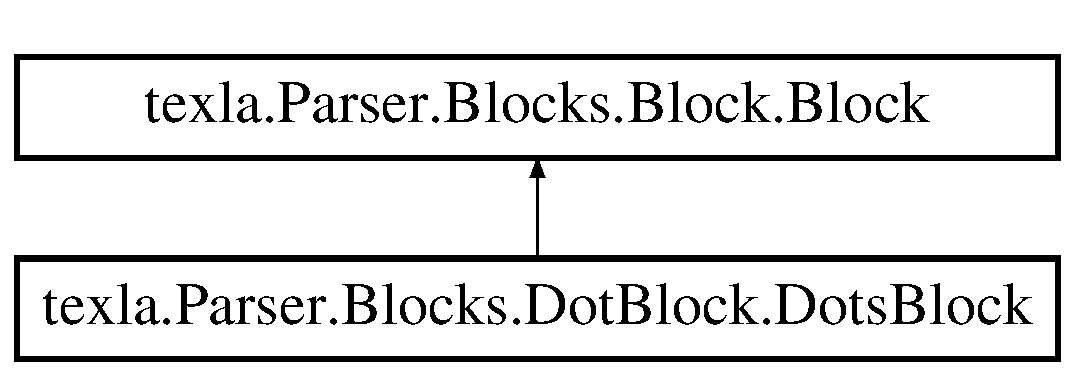
\includegraphics[height=2.000000cm]{classtexla_1_1Parser_1_1Blocks_1_1DotBlock_1_1DotsBlock}
\end{center}
\end{figure}
\subsection*{Public Member Functions}
\begin{DoxyCompactItemize}
\item 
\hypertarget{classtexla_1_1Parser_1_1Blocks_1_1DotBlock_1_1DotsBlock_aa9b718c90f1b7e2fe739af312bac9f41}{}\label{classtexla_1_1Parser_1_1Blocks_1_1DotBlock_1_1DotsBlock_aa9b718c90f1b7e2fe739af312bac9f41} 
def {\bfseries \+\_\+\+\_\+init\+\_\+\+\_\+} (self, dot\+\_\+type, parent\+\_\+block)
\item 
\hypertarget{classtexla_1_1Parser_1_1Blocks_1_1DotBlock_1_1DotsBlock_a55e745da687b817be13f2d467705f990}{}\label{classtexla_1_1Parser_1_1Blocks_1_1DotBlock_1_1DotsBlock_a55e745da687b817be13f2d467705f990} 
def {\bfseries \+\_\+\+\_\+str\+\_\+\+\_\+} (self)
\end{DoxyCompactItemize}
\subsection*{Static Public Member Functions}
\begin{DoxyCompactItemize}
\item 
\hypertarget{classtexla_1_1Parser_1_1Blocks_1_1DotBlock_1_1DotsBlock_a6a25a42bf852862b9861994a3347513f}{}\label{classtexla_1_1Parser_1_1Blocks_1_1DotBlock_1_1DotsBlock_a6a25a42bf852862b9861994a3347513f} 
def {\bfseries parse} (parser, tex, parent\+\_\+block, params)
\end{DoxyCompactItemize}
\subsection*{Public Attributes}
\begin{DoxyCompactItemize}
\item 
\hypertarget{classtexla_1_1Parser_1_1Blocks_1_1DotBlock_1_1DotsBlock_a1bc93499359c0302b98393051086f06f}{}\label{classtexla_1_1Parser_1_1Blocks_1_1DotBlock_1_1DotsBlock_a1bc93499359c0302b98393051086f06f} 
{\bfseries dot\+\_\+type}
\end{DoxyCompactItemize}


The documentation for this class was generated from the following file\+:\begin{DoxyCompactItemize}
\item 
texla/\+Parser/\+Blocks/Dot\+Block.\+py\end{DoxyCompactItemize}

\hypertarget{classtexla_1_1Parser_1_1Blocks_1_1FigureBlocks_1_1FigureBlock}{}\section{texla.\+Parser.\+Blocks.\+Figure\+Blocks.\+Figure\+Block Class Reference}
\label{classtexla_1_1Parser_1_1Blocks_1_1FigureBlocks_1_1FigureBlock}\index{texla.\+Parser.\+Blocks.\+Figure\+Blocks.\+Figure\+Block@{texla.\+Parser.\+Blocks.\+Figure\+Blocks.\+Figure\+Block}}
Inheritance diagram for texla.\+Parser.\+Blocks.\+Figure\+Blocks.\+Figure\+Block\+:\begin{figure}[H]
\begin{center}
\leavevmode
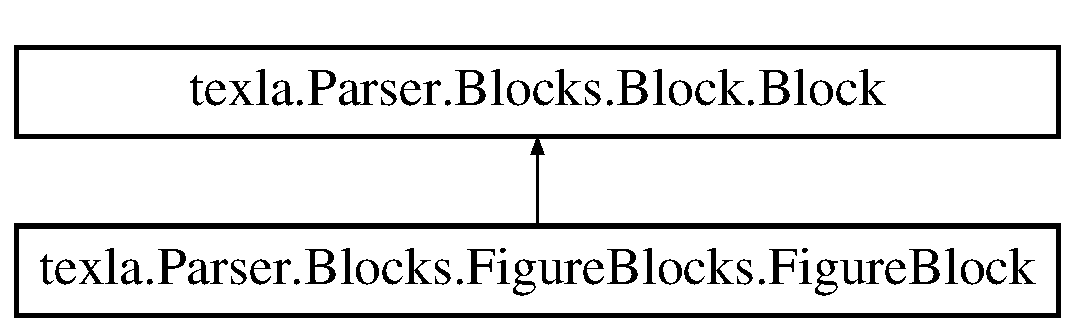
\includegraphics[height=2.000000cm]{classtexla_1_1Parser_1_1Blocks_1_1FigureBlocks_1_1FigureBlock}
\end{center}
\end{figure}
\subsection*{Public Member Functions}
\begin{DoxyCompactItemize}
\item 
\hypertarget{classtexla_1_1Parser_1_1Blocks_1_1FigureBlocks_1_1FigureBlock_a87e9d52d5cf3aa8a75d8be4997af262a}{}\label{classtexla_1_1Parser_1_1Blocks_1_1FigureBlocks_1_1FigureBlock_a87e9d52d5cf3aa8a75d8be4997af262a} 
def {\bfseries \+\_\+\+\_\+init\+\_\+\+\_\+} (self, placement\+\_\+specifier, tex, parent\+\_\+block)
\end{DoxyCompactItemize}
\subsection*{Static Public Member Functions}
\begin{DoxyCompactItemize}
\item 
\hypertarget{classtexla_1_1Parser_1_1Blocks_1_1FigureBlocks_1_1FigureBlock_a28e379084a4bff05e9e2923a5f2c4b17}{}\label{classtexla_1_1Parser_1_1Blocks_1_1FigureBlocks_1_1FigureBlock_a28e379084a4bff05e9e2923a5f2c4b17} 
def {\bfseries parse\+\_\+env} (parser, tex, parent\+\_\+block, params)
\end{DoxyCompactItemize}
\subsection*{Additional Inherited Members}


\subsection{Detailed Description}
\begin{DoxyVerb}Permission to place the float:
h here at the very place in the text where it occurred.
This is useful mainly for small floats.
t at the top of a page
b at the bottom of a page
p on a special page containing only floats.
! without considering most of the internal parametersa,
which could otherwhise stop this float from being placed.
\end{DoxyVerb}
 

The documentation for this class was generated from the following file\+:\begin{DoxyCompactItemize}
\item 
texla/\+Parser/\+Blocks/Figure\+Blocks.\+py\end{DoxyCompactItemize}

\hypertarget{classtexla_1_1Parser_1_1Blocks_1_1NoteBlocks_1_1FootnoteBlock}{}\section{texla.\+Parser.\+Blocks.\+Note\+Blocks.\+Footnote\+Block Class Reference}
\label{classtexla_1_1Parser_1_1Blocks_1_1NoteBlocks_1_1FootnoteBlock}\index{texla.\+Parser.\+Blocks.\+Note\+Blocks.\+Footnote\+Block@{texla.\+Parser.\+Blocks.\+Note\+Blocks.\+Footnote\+Block}}
Inheritance diagram for texla.\+Parser.\+Blocks.\+Note\+Blocks.\+Footnote\+Block\+:\begin{figure}[H]
\begin{center}
\leavevmode
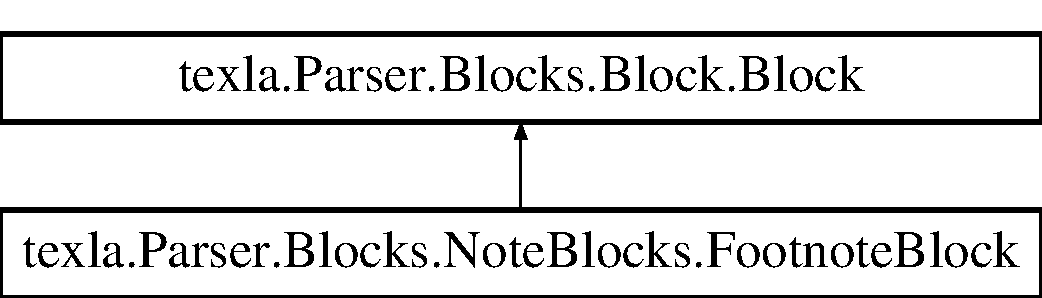
\includegraphics[height=2.000000cm]{classtexla_1_1Parser_1_1Blocks_1_1NoteBlocks_1_1FootnoteBlock}
\end{center}
\end{figure}
\subsection*{Public Member Functions}
\begin{DoxyCompactItemize}
\item 
\hypertarget{classtexla_1_1Parser_1_1Blocks_1_1NoteBlocks_1_1FootnoteBlock_aea7afb002614e686bc3d986e391cd389}{}\label{classtexla_1_1Parser_1_1Blocks_1_1NoteBlocks_1_1FootnoteBlock_aea7afb002614e686bc3d986e391cd389} 
def {\bfseries \+\_\+\+\_\+init\+\_\+\+\_\+} (self, tex, parent\+\_\+block)
\end{DoxyCompactItemize}
\subsection*{Static Public Member Functions}
\begin{DoxyCompactItemize}
\item 
\hypertarget{classtexla_1_1Parser_1_1Blocks_1_1NoteBlocks_1_1FootnoteBlock_acc57481997336bc8f78617fa7d76b9ab}{}\label{classtexla_1_1Parser_1_1Blocks_1_1NoteBlocks_1_1FootnoteBlock_acc57481997336bc8f78617fa7d76b9ab} 
def {\bfseries parse} (parser, tex, parent\+\_\+block, params)
\end{DoxyCompactItemize}
\subsection*{Additional Inherited Members}


\subsection{Detailed Description}
\begin{DoxyVerb}This class handles \footnote command\end{DoxyVerb}
 

The documentation for this class was generated from the following file\+:\begin{DoxyCompactItemize}
\item 
texla/\+Parser/\+Blocks/Note\+Blocks.\+py\end{DoxyCompactItemize}

\hypertarget{classtexla_1_1Parser_1_1Blocks_1_1FormattingBlocks_1_1FormattingGroupBlock}{}\section{texla.\+Parser.\+Blocks.\+Formatting\+Blocks.\+Formatting\+Group\+Block Class Reference}
\label{classtexla_1_1Parser_1_1Blocks_1_1FormattingBlocks_1_1FormattingGroupBlock}\index{texla.\+Parser.\+Blocks.\+Formatting\+Blocks.\+Formatting\+Group\+Block@{texla.\+Parser.\+Blocks.\+Formatting\+Blocks.\+Formatting\+Group\+Block}}
Inheritance diagram for texla.\+Parser.\+Blocks.\+Formatting\+Blocks.\+Formatting\+Group\+Block\+:\begin{figure}[H]
\begin{center}
\leavevmode
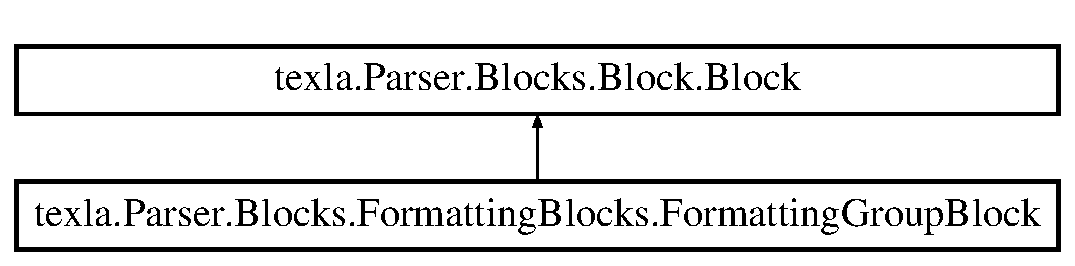
\includegraphics[height=2.000000cm]{classtexla_1_1Parser_1_1Blocks_1_1FormattingBlocks_1_1FormattingGroupBlock}
\end{center}
\end{figure}
\subsection*{Public Member Functions}
\begin{DoxyCompactItemize}
\item 
\hypertarget{classtexla_1_1Parser_1_1Blocks_1_1FormattingBlocks_1_1FormattingGroupBlock_af1a0e6710404f1f8f4e98d4abf8a99c7}{}\label{classtexla_1_1Parser_1_1Blocks_1_1FormattingBlocks_1_1FormattingGroupBlock_af1a0e6710404f1f8f4e98d4abf8a99c7} 
def {\bfseries \+\_\+\+\_\+init\+\_\+\+\_\+} (self, format\+\_\+type, parent\+\_\+block)
\end{DoxyCompactItemize}
\subsection*{Static Public Member Functions}
\begin{DoxyCompactItemize}
\item 
\hypertarget{classtexla_1_1Parser_1_1Blocks_1_1FormattingBlocks_1_1FormattingGroupBlock_a56fb6ea61a4e73c09f415de85e3c59e4}{}\label{classtexla_1_1Parser_1_1Blocks_1_1FormattingBlocks_1_1FormattingGroupBlock_a56fb6ea61a4e73c09f415de85e3c59e4} 
def {\bfseries parse} (parser, tex, parent\+\_\+block, params)
\end{DoxyCompactItemize}
\subsection*{Additional Inherited Members}


\subsection{Detailed Description}
\begin{DoxyVerb}This type of block is created for formatting
commands used inside a {...} construct\end{DoxyVerb}
 

The documentation for this class was generated from the following file\+:\begin{DoxyCompactItemize}
\item 
texla/\+Parser/\+Blocks/Formatting\+Blocks.\+py\end{DoxyCompactItemize}

\hypertarget{classtexla_1_1Parser_1_1Blocks_1_1FormattingBlocks_1_1FormattingTextBlock}{}\section{texla.\+Parser.\+Blocks.\+Formatting\+Blocks.\+Formatting\+Text\+Block Class Reference}
\label{classtexla_1_1Parser_1_1Blocks_1_1FormattingBlocks_1_1FormattingTextBlock}\index{texla.\+Parser.\+Blocks.\+Formatting\+Blocks.\+Formatting\+Text\+Block@{texla.\+Parser.\+Blocks.\+Formatting\+Blocks.\+Formatting\+Text\+Block}}
Inheritance diagram for texla.\+Parser.\+Blocks.\+Formatting\+Blocks.\+Formatting\+Text\+Block\+:\begin{figure}[H]
\begin{center}
\leavevmode
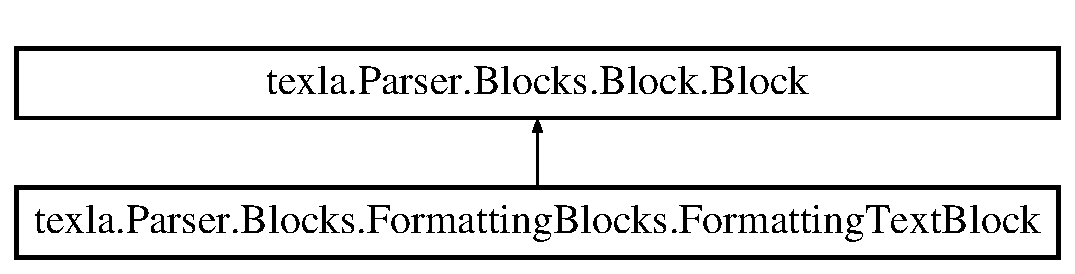
\includegraphics[height=2.000000cm]{classtexla_1_1Parser_1_1Blocks_1_1FormattingBlocks_1_1FormattingTextBlock}
\end{center}
\end{figure}
\subsection*{Public Member Functions}
\begin{DoxyCompactItemize}
\item 
\hypertarget{classtexla_1_1Parser_1_1Blocks_1_1FormattingBlocks_1_1FormattingTextBlock_a21cbd1ee74f54c27c1f0911cac3d62b0}{}\label{classtexla_1_1Parser_1_1Blocks_1_1FormattingBlocks_1_1FormattingTextBlock_a21cbd1ee74f54c27c1f0911cac3d62b0} 
def {\bfseries \+\_\+\+\_\+init\+\_\+\+\_\+} (self, format\+\_\+type, text, parent\+\_\+block)
\end{DoxyCompactItemize}
\subsection*{Static Public Member Functions}
\begin{DoxyCompactItemize}
\item 
\hypertarget{classtexla_1_1Parser_1_1Blocks_1_1FormattingBlocks_1_1FormattingTextBlock_a73841619b03e29bf293e1f465a54b464}{}\label{classtexla_1_1Parser_1_1Blocks_1_1FormattingBlocks_1_1FormattingTextBlock_a73841619b03e29bf293e1f465a54b464} 
def {\bfseries parse} (parser, tex, parent\+\_\+block, params)
\end{DoxyCompactItemize}
\subsection*{Additional Inherited Members}


The documentation for this class was generated from the following file\+:\begin{DoxyCompactItemize}
\item 
texla/\+Parser/\+Blocks/Formatting\+Blocks.\+py\end{DoxyCompactItemize}

\hypertarget{classtexla_1_1Parser_1_1Blocks_1_1HeaderBlock_1_1HeaderBlock}{}\section{texla.\+Parser.\+Blocks.\+Header\+Block.\+Header\+Block Class Reference}
\label{classtexla_1_1Parser_1_1Blocks_1_1HeaderBlock_1_1HeaderBlock}\index{texla.\+Parser.\+Blocks.\+Header\+Block.\+Header\+Block@{texla.\+Parser.\+Blocks.\+Header\+Block.\+Header\+Block}}
Inheritance diagram for texla.\+Parser.\+Blocks.\+Header\+Block.\+Header\+Block\+:\begin{figure}[H]
\begin{center}
\leavevmode
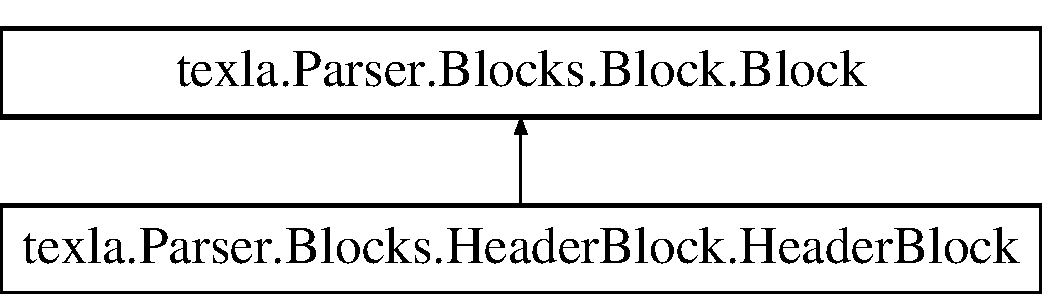
\includegraphics[height=2.000000cm]{classtexla_1_1Parser_1_1Blocks_1_1HeaderBlock_1_1HeaderBlock}
\end{center}
\end{figure}
\subsection*{Public Member Functions}
\begin{DoxyCompactItemize}
\item 
\hypertarget{classtexla_1_1Parser_1_1Blocks_1_1HeaderBlock_1_1HeaderBlock_a7d9694b33f4546835215718b140a13b0}{}\label{classtexla_1_1Parser_1_1Blocks_1_1HeaderBlock_1_1HeaderBlock_a7d9694b33f4546835215718b140a13b0} 
def {\bfseries \+\_\+\+\_\+init\+\_\+\+\_\+} (self, title, date, author, parent\+\_\+block)
\end{DoxyCompactItemize}
\subsection*{Static Public Member Functions}
\begin{DoxyCompactItemize}
\item 
\hypertarget{classtexla_1_1Parser_1_1Blocks_1_1HeaderBlock_1_1HeaderBlock_a66a2af1f4724e15cc28c5593c37c4152}{}\label{classtexla_1_1Parser_1_1Blocks_1_1HeaderBlock_1_1HeaderBlock_a66a2af1f4724e15cc28c5593c37c4152} 
def {\bfseries parse} (parser, tex, parent\+\_\+block, params)
\end{DoxyCompactItemize}
\subsection*{Additional Inherited Members}


\subsection{Detailed Description}
\begin{DoxyVerb}This class get title,author and date at the beginning of tex\end{DoxyVerb}
 

The documentation for this class was generated from the following file\+:\begin{DoxyCompactItemize}
\item 
texla/\+Parser/\+Blocks/Header\+Block.\+py\end{DoxyCompactItemize}

\hypertarget{classtexla_1_1Parser_1_1Blocks_1_1TabularBlocks_1_1HlineBlock}{}\section{texla.\+Parser.\+Blocks.\+Tabular\+Blocks.\+Hline\+Block Class Reference}
\label{classtexla_1_1Parser_1_1Blocks_1_1TabularBlocks_1_1HlineBlock}\index{texla.\+Parser.\+Blocks.\+Tabular\+Blocks.\+Hline\+Block@{texla.\+Parser.\+Blocks.\+Tabular\+Blocks.\+Hline\+Block}}
Inheritance diagram for texla.\+Parser.\+Blocks.\+Tabular\+Blocks.\+Hline\+Block\+:\begin{figure}[H]
\begin{center}
\leavevmode
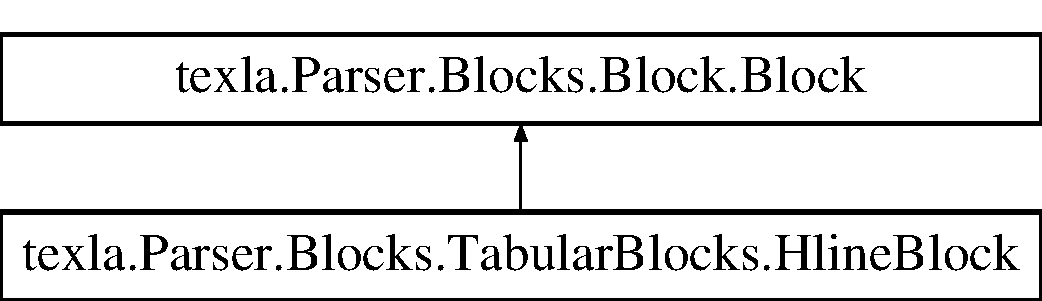
\includegraphics[height=2.000000cm]{classtexla_1_1Parser_1_1Blocks_1_1TabularBlocks_1_1HlineBlock}
\end{center}
\end{figure}
\subsection*{Public Member Functions}
\begin{DoxyCompactItemize}
\item 
\hypertarget{classtexla_1_1Parser_1_1Blocks_1_1TabularBlocks_1_1HlineBlock_a9d8482d681c49219ff2b99318d0723ae}{}\label{classtexla_1_1Parser_1_1Blocks_1_1TabularBlocks_1_1HlineBlock_a9d8482d681c49219ff2b99318d0723ae} 
def {\bfseries parse} (parser, tex, parent\+\_\+block, params)
\item 
\hypertarget{classtexla_1_1Parser_1_1Blocks_1_1TabularBlocks_1_1HlineBlock_a40f4c1e692bc7acfe8b33ace58749c62}{}\label{classtexla_1_1Parser_1_1Blocks_1_1TabularBlocks_1_1HlineBlock_a40f4c1e692bc7acfe8b33ace58749c62} 
def {\bfseries \+\_\+\+\_\+init\+\_\+\+\_\+} (self, parent\+\_\+block)
\end{DoxyCompactItemize}
\subsection*{Additional Inherited Members}


The documentation for this class was generated from the following file\+:\begin{DoxyCompactItemize}
\item 
texla/\+Parser/\+Blocks/Tabular\+Blocks.\+py\end{DoxyCompactItemize}

\hypertarget{classtexla_1_1Parser_1_1Blocks_1_1FigureBlocks_1_1IncludeGraphicsBlock}{}\section{texla.\+Parser.\+Blocks.\+Figure\+Blocks.\+Include\+Graphics\+Block Class Reference}
\label{classtexla_1_1Parser_1_1Blocks_1_1FigureBlocks_1_1IncludeGraphicsBlock}\index{texla.\+Parser.\+Blocks.\+Figure\+Blocks.\+Include\+Graphics\+Block@{texla.\+Parser.\+Blocks.\+Figure\+Blocks.\+Include\+Graphics\+Block}}
Inheritance diagram for texla.\+Parser.\+Blocks.\+Figure\+Blocks.\+Include\+Graphics\+Block\+:\begin{figure}[H]
\begin{center}
\leavevmode
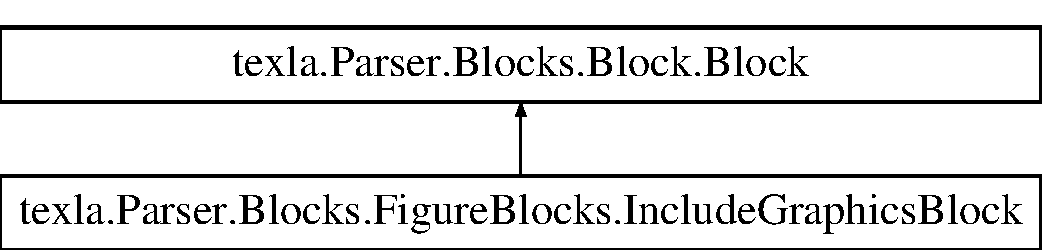
\includegraphics[height=2.000000cm]{classtexla_1_1Parser_1_1Blocks_1_1FigureBlocks_1_1IncludeGraphicsBlock}
\end{center}
\end{figure}
\subsection*{Public Member Functions}
\begin{DoxyCompactItemize}
\item 
\hypertarget{classtexla_1_1Parser_1_1Blocks_1_1FigureBlocks_1_1IncludeGraphicsBlock_a93ccc4cb679dfb2a036f0ab875ba7e75}{}\label{classtexla_1_1Parser_1_1Blocks_1_1FigureBlocks_1_1IncludeGraphicsBlock_a93ccc4cb679dfb2a036f0ab875ba7e75} 
def {\bfseries \+\_\+\+\_\+init\+\_\+\+\_\+} (self, img\+\_\+name, ar\+\_\+img\+\_\+info, tex, parent\+\_\+block)
\end{DoxyCompactItemize}
\subsection*{Static Public Member Functions}
\begin{DoxyCompactItemize}
\item 
\hypertarget{classtexla_1_1Parser_1_1Blocks_1_1FigureBlocks_1_1IncludeGraphicsBlock_abf8847a83e889f0c1228e7a261e51495}{}\label{classtexla_1_1Parser_1_1Blocks_1_1FigureBlocks_1_1IncludeGraphicsBlock_abf8847a83e889f0c1228e7a261e51495} 
def {\bfseries parse} (parser, tex, parent\+\_\+block, params)
\end{DoxyCompactItemize}
\subsection*{Additional Inherited Members}


The documentation for this class was generated from the following file\+:\begin{DoxyCompactItemize}
\item 
texla/\+Parser/\+Blocks/Figure\+Blocks.\+py\end{DoxyCompactItemize}

\hypertarget{classtexla_1_1Parser_1_1Blocks_1_1ListBlocks_1_1ItemBlock}{}\section{texla.\+Parser.\+Blocks.\+List\+Blocks.\+Item\+Block Class Reference}
\label{classtexla_1_1Parser_1_1Blocks_1_1ListBlocks_1_1ItemBlock}\index{texla.\+Parser.\+Blocks.\+List\+Blocks.\+Item\+Block@{texla.\+Parser.\+Blocks.\+List\+Blocks.\+Item\+Block}}
Inheritance diagram for texla.\+Parser.\+Blocks.\+List\+Blocks.\+Item\+Block\+:\begin{figure}[H]
\begin{center}
\leavevmode
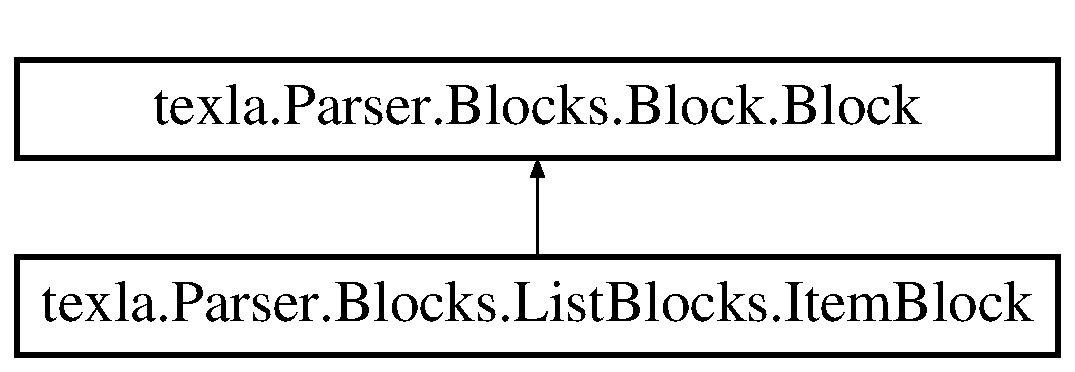
\includegraphics[height=2.000000cm]{classtexla_1_1Parser_1_1Blocks_1_1ListBlocks_1_1ItemBlock}
\end{center}
\end{figure}
\subsection*{Public Member Functions}
\begin{DoxyCompactItemize}
\item 
\hypertarget{classtexla_1_1Parser_1_1Blocks_1_1ListBlocks_1_1ItemBlock_ad505df66f3879578d353543bebf257ff}{}\label{classtexla_1_1Parser_1_1Blocks_1_1ListBlocks_1_1ItemBlock_ad505df66f3879578d353543bebf257ff} 
def {\bfseries \+\_\+\+\_\+init\+\_\+\+\_\+} (self, word, parent\+\_\+block)
\end{DoxyCompactItemize}
\subsection*{Static Public Member Functions}
\begin{DoxyCompactItemize}
\item 
\hypertarget{classtexla_1_1Parser_1_1Blocks_1_1ListBlocks_1_1ItemBlock_a99fa94bc5834b7df4765bb3864b7b979}{}\label{classtexla_1_1Parser_1_1Blocks_1_1ListBlocks_1_1ItemBlock_a99fa94bc5834b7df4765bb3864b7b979} 
def {\bfseries parse} (parser, tex, parent\+\_\+block, params)
\end{DoxyCompactItemize}
\subsection*{Additional Inherited Members}


\subsection{Detailed Description}
\begin{DoxyVerb}This is only a place holder for a item.
The itemize environment will add it his content.
It's impossibile to extract it before\end{DoxyVerb}
 

The documentation for this class was generated from the following file\+:\begin{DoxyCompactItemize}
\item 
texla/\+Parser/\+Blocks/List\+Blocks.\+py\end{DoxyCompactItemize}

\hypertarget{classtexla_1_1Parser_1_1Blocks_1_1ReferenceBlocks_1_1LabelBlock}{}\section{texla.\+Parser.\+Blocks.\+Reference\+Blocks.\+Label\+Block Class Reference}
\label{classtexla_1_1Parser_1_1Blocks_1_1ReferenceBlocks_1_1LabelBlock}\index{texla.\+Parser.\+Blocks.\+Reference\+Blocks.\+Label\+Block@{texla.\+Parser.\+Blocks.\+Reference\+Blocks.\+Label\+Block}}
Inheritance diagram for texla.\+Parser.\+Blocks.\+Reference\+Blocks.\+Label\+Block\+:\begin{figure}[H]
\begin{center}
\leavevmode
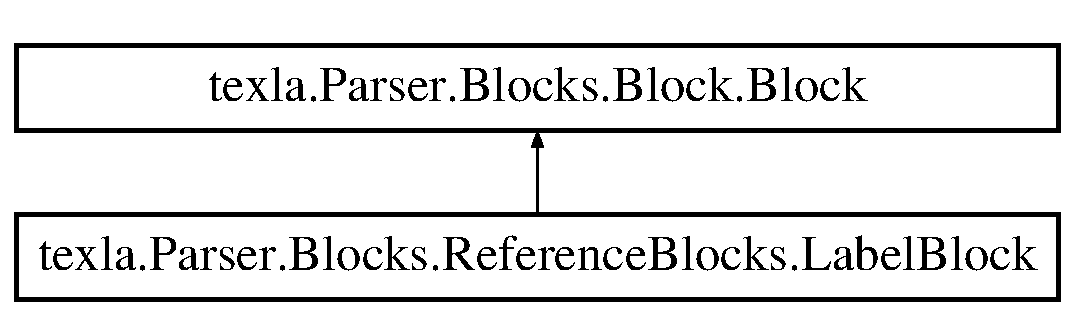
\includegraphics[height=2.000000cm]{classtexla_1_1Parser_1_1Blocks_1_1ReferenceBlocks_1_1LabelBlock}
\end{center}
\end{figure}
\subsection*{Public Member Functions}
\begin{DoxyCompactItemize}
\item 
\hypertarget{classtexla_1_1Parser_1_1Blocks_1_1ReferenceBlocks_1_1LabelBlock_a91cae105c96931e4b0c02f01e095c3da}{}\label{classtexla_1_1Parser_1_1Blocks_1_1ReferenceBlocks_1_1LabelBlock_a91cae105c96931e4b0c02f01e095c3da} 
def {\bfseries \+\_\+\+\_\+init\+\_\+\+\_\+} (self, label, parent\+\_\+block)
\item 
\hypertarget{classtexla_1_1Parser_1_1Blocks_1_1ReferenceBlocks_1_1LabelBlock_ae4858d4d10980aab8cb6d5a8eeb90a31}{}\label{classtexla_1_1Parser_1_1Blocks_1_1ReferenceBlocks_1_1LabelBlock_ae4858d4d10980aab8cb6d5a8eeb90a31} 
def {\bfseries \+\_\+\+\_\+str\+\_\+\+\_\+} (self)
\end{DoxyCompactItemize}
\subsection*{Static Public Member Functions}
\begin{DoxyCompactItemize}
\item 
\hypertarget{classtexla_1_1Parser_1_1Blocks_1_1ReferenceBlocks_1_1LabelBlock_ad3e9c07484143a2d3000d79a49ddefaf}{}\label{classtexla_1_1Parser_1_1Blocks_1_1ReferenceBlocks_1_1LabelBlock_ad3e9c07484143a2d3000d79a49ddefaf} 
def {\bfseries parse\+\_\+label} (parser, tex, parent\+\_\+block, params)
\end{DoxyCompactItemize}
\subsection*{Public Attributes}
\begin{DoxyCompactItemize}
\item 
\hypertarget{classtexla_1_1Parser_1_1Blocks_1_1ReferenceBlocks_1_1LabelBlock_af85aa3c1e5b6ca49e436b4daedc8fe2f}{}\label{classtexla_1_1Parser_1_1Blocks_1_1ReferenceBlocks_1_1LabelBlock_af85aa3c1e5b6ca49e436b4daedc8fe2f} 
{\bfseries label}
\end{DoxyCompactItemize}


\subsection{Detailed Description}
\begin{DoxyVerb}Block that represents labels\end{DoxyVerb}
 

The documentation for this class was generated from the following file\+:\begin{DoxyCompactItemize}
\item 
texla/\+Parser/\+Blocks/Reference\+Blocks.\+py\end{DoxyCompactItemize}

\hypertarget{classtexla_1_1Parser_1_1Blocks_1_1ListBlocks_1_1ListBlock}{}\section{texla.\+Parser.\+Blocks.\+List\+Blocks.\+List\+Block Class Reference}
\label{classtexla_1_1Parser_1_1Blocks_1_1ListBlocks_1_1ListBlock}\index{texla.\+Parser.\+Blocks.\+List\+Blocks.\+List\+Block@{texla.\+Parser.\+Blocks.\+List\+Blocks.\+List\+Block}}
Inheritance diagram for texla.\+Parser.\+Blocks.\+List\+Blocks.\+List\+Block\+:\begin{figure}[H]
\begin{center}
\leavevmode
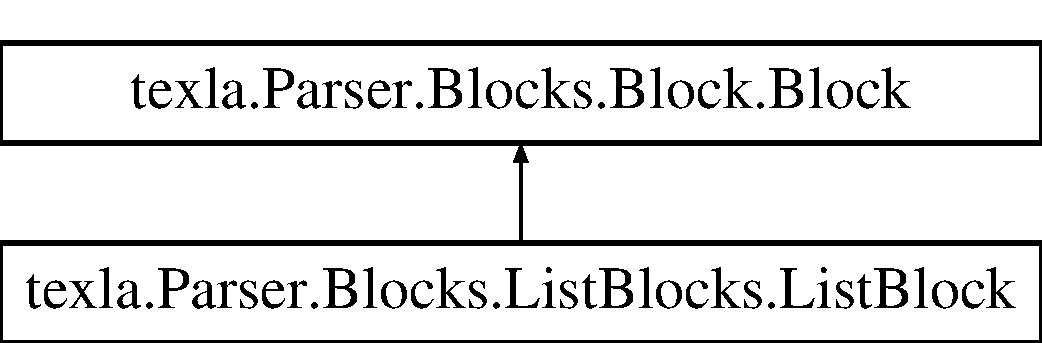
\includegraphics[height=2.000000cm]{classtexla_1_1Parser_1_1Blocks_1_1ListBlocks_1_1ListBlock}
\end{center}
\end{figure}
\subsection*{Public Member Functions}
\begin{DoxyCompactItemize}
\item 
\hypertarget{classtexla_1_1Parser_1_1Blocks_1_1ListBlocks_1_1ListBlock_a72828e3b10fc6a6c22f6afed383af95e}{}\label{classtexla_1_1Parser_1_1Blocks_1_1ListBlocks_1_1ListBlock_a72828e3b10fc6a6c22f6afed383af95e} 
def {\bfseries \+\_\+\+\_\+init\+\_\+\+\_\+} (self, list\+\_\+type, tex, parent\+\_\+block)
\end{DoxyCompactItemize}
\subsection*{Static Public Member Functions}
\begin{DoxyCompactItemize}
\item 
def \hyperlink{classtexla_1_1Parser_1_1Blocks_1_1ListBlocks_1_1ListBlock_aaf69903ae29fb0d00539f91c6db5a656}{parse} (parser, tex, parent\+\_\+block, params)
\end{DoxyCompactItemize}
\subsection*{Additional Inherited Members}


\subsection{Detailed Description}
\begin{DoxyVerb}We use one Block type for all listings.
Itemize, Enumerate, Description are
specified in list_type attributes.
\end{DoxyVerb}
 

\subsection{Member Function Documentation}
\hypertarget{classtexla_1_1Parser_1_1Blocks_1_1ListBlocks_1_1ListBlock_aaf69903ae29fb0d00539f91c6db5a656}{}\label{classtexla_1_1Parser_1_1Blocks_1_1ListBlocks_1_1ListBlock_aaf69903ae29fb0d00539f91c6db5a656} 
\index{texla\+::\+Parser\+::\+Blocks\+::\+List\+Blocks\+::\+List\+Block@{texla\+::\+Parser\+::\+Blocks\+::\+List\+Blocks\+::\+List\+Block}!parse@{parse}}
\index{parse@{parse}!texla\+::\+Parser\+::\+Blocks\+::\+List\+Blocks\+::\+List\+Block@{texla\+::\+Parser\+::\+Blocks\+::\+List\+Blocks\+::\+List\+Block}}
\subsubsection{\texorpdfstring{parse()}{parse()}}
{\footnotesize\ttfamily def texla.\+Parser.\+Blocks.\+List\+Blocks.\+List\+Block.\+parse (\begin{DoxyParamCaption}\item[{}]{parser,  }\item[{}]{tex,  }\item[{}]{parent\+\_\+block,  }\item[{}]{params }\end{DoxyParamCaption})\hspace{0.3cm}{\ttfamily [static]}}

\begin{DoxyVerb}We parse the content of the env.
Then we analyze the blocks and find
which are items and not. The hierarchy of
blocks is constructed after the parsing of
the content. It's the only way to let the parser
handle nested environments. Then, all the
blocks are reappended under items blocks and
added as children nodes.
\end{DoxyVerb}
 

The documentation for this class was generated from the following file\+:\begin{DoxyCompactItemize}
\item 
texla/\+Parser/\+Blocks/List\+Blocks.\+py\end{DoxyCompactItemize}

\hypertarget{classtexla_1_1Parser_1_1Blocks_1_1Utilities_1_1MacroParser_1_1Macro}{}\section{texla.\+Parser.\+Blocks.\+Utilities.\+Macro\+Parser.\+Macro Class Reference}
\label{classtexla_1_1Parser_1_1Blocks_1_1Utilities_1_1MacroParser_1_1Macro}\index{texla.\+Parser.\+Blocks.\+Utilities.\+Macro\+Parser.\+Macro@{texla.\+Parser.\+Blocks.\+Utilities.\+Macro\+Parser.\+Macro}}
\subsection*{Public Member Functions}
\begin{DoxyCompactItemize}
\item 
\hypertarget{classtexla_1_1Parser_1_1Blocks_1_1Utilities_1_1MacroParser_1_1Macro_abbe07cf46b4432ce9a65e576718c5bf2}{}\label{classtexla_1_1Parser_1_1Blocks_1_1Utilities_1_1MacroParser_1_1Macro_abbe07cf46b4432ce9a65e576718c5bf2} 
def {\bfseries \+\_\+\+\_\+init\+\_\+\+\_\+} (self, name, n\+\_\+param, default, content)
\item 
def \hyperlink{classtexla_1_1Parser_1_1Blocks_1_1Utilities_1_1MacroParser_1_1Macro_a7f605660a8517687a8b13cfa51637047}{get\+\_\+tex} (self, params, param\+\_\+default=None)
\end{DoxyCompactItemize}
\subsection*{Static Public Member Functions}
\begin{DoxyCompactItemize}
\item 
def \hyperlink{classtexla_1_1Parser_1_1Blocks_1_1Utilities_1_1MacroParser_1_1Macro_a874a31f4bd9da2ccc4f949656b12b23c}{parse\+\_\+macro} (tex)
\end{DoxyCompactItemize}
\subsection*{Public Attributes}
\begin{DoxyCompactItemize}
\item 
\hypertarget{classtexla_1_1Parser_1_1Blocks_1_1Utilities_1_1MacroParser_1_1Macro_a0cc551d407614256f3fe8cfc497ab035}{}\label{classtexla_1_1Parser_1_1Blocks_1_1Utilities_1_1MacroParser_1_1Macro_a0cc551d407614256f3fe8cfc497ab035} 
{\bfseries name}
\item 
\hypertarget{classtexla_1_1Parser_1_1Blocks_1_1Utilities_1_1MacroParser_1_1Macro_aaadac96ac5b3068207eaffdd876ed7dd}{}\label{classtexla_1_1Parser_1_1Blocks_1_1Utilities_1_1MacroParser_1_1Macro_aaadac96ac5b3068207eaffdd876ed7dd} 
{\bfseries n\+\_\+param}
\item 
\hypertarget{classtexla_1_1Parser_1_1Blocks_1_1Utilities_1_1MacroParser_1_1Macro_ae29386b4c41336f5d171da8e39239cbd}{}\label{classtexla_1_1Parser_1_1Blocks_1_1Utilities_1_1MacroParser_1_1Macro_ae29386b4c41336f5d171da8e39239cbd} 
{\bfseries default}
\item 
\hypertarget{classtexla_1_1Parser_1_1Blocks_1_1Utilities_1_1MacroParser_1_1Macro_a15723fef45ee5c9e860b3a5c27303b1b}{}\label{classtexla_1_1Parser_1_1Blocks_1_1Utilities_1_1MacroParser_1_1Macro_a15723fef45ee5c9e860b3a5c27303b1b} 
{\bfseries content}
\end{DoxyCompactItemize}


\subsection{Detailed Description}
\begin{DoxyVerb}This class represents a Latex macro, a
newcommands. It saves the definition of the macro
and it's able to recreate the tex replacement of the macro
given the params parsed.\end{DoxyVerb}
 

\subsection{Member Function Documentation}
\hypertarget{classtexla_1_1Parser_1_1Blocks_1_1Utilities_1_1MacroParser_1_1Macro_a7f605660a8517687a8b13cfa51637047}{}\label{classtexla_1_1Parser_1_1Blocks_1_1Utilities_1_1MacroParser_1_1Macro_a7f605660a8517687a8b13cfa51637047} 
\index{texla\+::\+Parser\+::\+Blocks\+::\+Utilities\+::\+Macro\+Parser\+::\+Macro@{texla\+::\+Parser\+::\+Blocks\+::\+Utilities\+::\+Macro\+Parser\+::\+Macro}!get\+\_\+tex@{get\+\_\+tex}}
\index{get\+\_\+tex@{get\+\_\+tex}!texla\+::\+Parser\+::\+Blocks\+::\+Utilities\+::\+Macro\+Parser\+::\+Macro@{texla\+::\+Parser\+::\+Blocks\+::\+Utilities\+::\+Macro\+Parser\+::\+Macro}}
\subsubsection{\texorpdfstring{get\+\_\+tex()}{get\_tex()}}
{\footnotesize\ttfamily def texla.\+Parser.\+Blocks.\+Utilities.\+Macro\+Parser.\+Macro.\+get\+\_\+tex (\begin{DoxyParamCaption}\item[{}]{self,  }\item[{}]{params,  }\item[{}]{param\+\_\+default = {\ttfamily None} }\end{DoxyParamCaption})}

\begin{DoxyVerb}This function return the tex replacement for the
macro given a list of ordered parameters and,
if present, the default param (inside [...]).
\end{DoxyVerb}
 \hypertarget{classtexla_1_1Parser_1_1Blocks_1_1Utilities_1_1MacroParser_1_1Macro_a874a31f4bd9da2ccc4f949656b12b23c}{}\label{classtexla_1_1Parser_1_1Blocks_1_1Utilities_1_1MacroParser_1_1Macro_a874a31f4bd9da2ccc4f949656b12b23c} 
\index{texla\+::\+Parser\+::\+Blocks\+::\+Utilities\+::\+Macro\+Parser\+::\+Macro@{texla\+::\+Parser\+::\+Blocks\+::\+Utilities\+::\+Macro\+Parser\+::\+Macro}!parse\+\_\+macro@{parse\+\_\+macro}}
\index{parse\+\_\+macro@{parse\+\_\+macro}!texla\+::\+Parser\+::\+Blocks\+::\+Utilities\+::\+Macro\+Parser\+::\+Macro@{texla\+::\+Parser\+::\+Blocks\+::\+Utilities\+::\+Macro\+Parser\+::\+Macro}}
\subsubsection{\texorpdfstring{parse\+\_\+macro()}{parse\_macro()}}
{\footnotesize\ttfamily def texla.\+Parser.\+Blocks.\+Utilities.\+Macro\+Parser.\+Macro.\+parse\+\_\+macro (\begin{DoxyParamCaption}\item[{}]{tex }\end{DoxyParamCaption})\hspace{0.3cm}{\ttfamily [static]}}

\begin{DoxyVerb}The function need the options part of the
\newcommand command, withoud newcommand. It returns the
parsed Macro object.
\end{DoxyVerb}
 

The documentation for this class was generated from the following file\+:\begin{DoxyCompactItemize}
\item 
texla/\+Parser/\+Blocks/\+Utilities/Macro\+Parser.\+py\end{DoxyCompactItemize}

\hypertarget{classtexla_1_1Parser_1_1Blocks_1_1MathBlocks_1_1MathBlock}{}\section{texla.\+Parser.\+Blocks.\+Math\+Blocks.\+Math\+Block Class Reference}
\label{classtexla_1_1Parser_1_1Blocks_1_1MathBlocks_1_1MathBlock}\index{texla.\+Parser.\+Blocks.\+Math\+Blocks.\+Math\+Block@{texla.\+Parser.\+Blocks.\+Math\+Blocks.\+Math\+Block}}
Inheritance diagram for texla.\+Parser.\+Blocks.\+Math\+Blocks.\+Math\+Block\+:\begin{figure}[H]
\begin{center}
\leavevmode
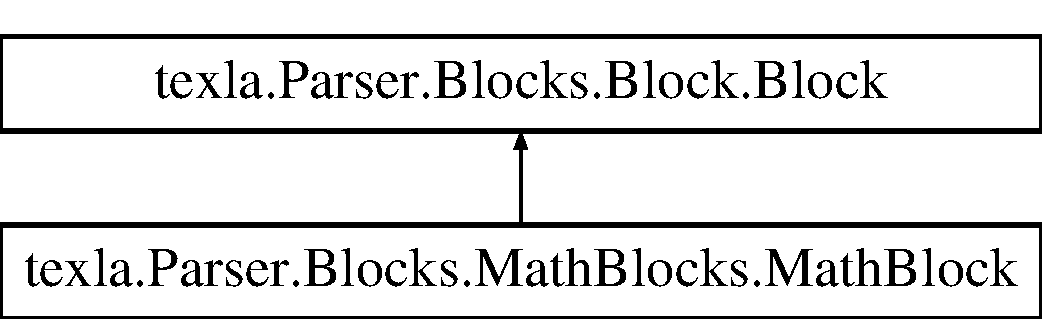
\includegraphics[height=2.000000cm]{classtexla_1_1Parser_1_1Blocks_1_1MathBlocks_1_1MathBlock}
\end{center}
\end{figure}
\subsection*{Public Member Functions}
\begin{DoxyCompactItemize}
\item 
\hypertarget{classtexla_1_1Parser_1_1Blocks_1_1MathBlocks_1_1MathBlock_aad8c1b85cdbff22d1ba54ad05afaec37}{}\label{classtexla_1_1Parser_1_1Blocks_1_1MathBlocks_1_1MathBlock_aad8c1b85cdbff22d1ba54ad05afaec37} 
def {\bfseries \+\_\+\+\_\+init\+\_\+\+\_\+} (self, math\+\_\+type, star, tex, parent\+\_\+block)
\item 
\hypertarget{classtexla_1_1Parser_1_1Blocks_1_1MathBlocks_1_1MathBlock_a50441f166a75cb41b14acc2f54005fdd}{}\label{classtexla_1_1Parser_1_1Blocks_1_1MathBlocks_1_1MathBlock_a50441f166a75cb41b14acc2f54005fdd} 
def {\bfseries \+\_\+\+\_\+str\+\_\+\+\_\+} (self)
\end{DoxyCompactItemize}
\subsection*{Static Public Member Functions}
\begin{DoxyCompactItemize}
\item 
def \hyperlink{classtexla_1_1Parser_1_1Blocks_1_1MathBlocks_1_1MathBlock_ac8726dcbb217a6fe85cfd493967bc88e}{parse\+\_\+math\+\_\+env} (parser, tex, parent\+\_\+block, params)
\item 
def \hyperlink{classtexla_1_1Parser_1_1Blocks_1_1MathBlocks_1_1MathBlock_a1042d3f5eb3d461418397c8f02695dc6}{parse\+\_\+ensure\+\_\+math} (parser, tex, parent\+\_\+block, params)
\item 
def \hyperlink{classtexla_1_1Parser_1_1Blocks_1_1MathBlocks_1_1MathBlock_a0cfddf038e1062d9f24763dc604bebdb}{parse\+\_\+labels} (tex)
\end{DoxyCompactItemize}
\subsection*{Public Attributes}
\begin{DoxyCompactItemize}
\item 
\hypertarget{classtexla_1_1Parser_1_1Blocks_1_1MathBlocks_1_1MathBlock_ab2667d65f7614809925dcd7252c6299b}{}\label{classtexla_1_1Parser_1_1Blocks_1_1MathBlocks_1_1MathBlock_ab2667d65f7614809925dcd7252c6299b} 
{\bfseries math\+\_\+type}
\item 
\hypertarget{classtexla_1_1Parser_1_1Blocks_1_1MathBlocks_1_1MathBlock_a112bfecb789c6797b2568c70e66abca0}{}\label{classtexla_1_1Parser_1_1Blocks_1_1MathBlocks_1_1MathBlock_a112bfecb789c6797b2568c70e66abca0} 
{\bfseries labels}
\end{DoxyCompactItemize}


\subsection{Member Function Documentation}
\hypertarget{classtexla_1_1Parser_1_1Blocks_1_1MathBlocks_1_1MathBlock_a1042d3f5eb3d461418397c8f02695dc6}{}\label{classtexla_1_1Parser_1_1Blocks_1_1MathBlocks_1_1MathBlock_a1042d3f5eb3d461418397c8f02695dc6} 
\index{texla\+::\+Parser\+::\+Blocks\+::\+Math\+Blocks\+::\+Math\+Block@{texla\+::\+Parser\+::\+Blocks\+::\+Math\+Blocks\+::\+Math\+Block}!parse\+\_\+ensure\+\_\+math@{parse\+\_\+ensure\+\_\+math}}
\index{parse\+\_\+ensure\+\_\+math@{parse\+\_\+ensure\+\_\+math}!texla\+::\+Parser\+::\+Blocks\+::\+Math\+Blocks\+::\+Math\+Block@{texla\+::\+Parser\+::\+Blocks\+::\+Math\+Blocks\+::\+Math\+Block}}
\subsubsection{\texorpdfstring{parse\+\_\+ensure\+\_\+math()}{parse\_ensure\_math()}}
{\footnotesize\ttfamily def texla.\+Parser.\+Blocks.\+Math\+Blocks.\+Math\+Block.\+parse\+\_\+ensure\+\_\+math (\begin{DoxyParamCaption}\item[{}]{parser,  }\item[{}]{tex,  }\item[{}]{parent\+\_\+block,  }\item[{}]{params }\end{DoxyParamCaption})\hspace{0.3cm}{\ttfamily [static]}}

\begin{DoxyVerb}The \ensuremath{} is a math command, not env\end{DoxyVerb}
 \hypertarget{classtexla_1_1Parser_1_1Blocks_1_1MathBlocks_1_1MathBlock_a0cfddf038e1062d9f24763dc604bebdb}{}\label{classtexla_1_1Parser_1_1Blocks_1_1MathBlocks_1_1MathBlock_a0cfddf038e1062d9f24763dc604bebdb} 
\index{texla\+::\+Parser\+::\+Blocks\+::\+Math\+Blocks\+::\+Math\+Block@{texla\+::\+Parser\+::\+Blocks\+::\+Math\+Blocks\+::\+Math\+Block}!parse\+\_\+labels@{parse\+\_\+labels}}
\index{parse\+\_\+labels@{parse\+\_\+labels}!texla\+::\+Parser\+::\+Blocks\+::\+Math\+Blocks\+::\+Math\+Block@{texla\+::\+Parser\+::\+Blocks\+::\+Math\+Blocks\+::\+Math\+Block}}
\subsubsection{\texorpdfstring{parse\+\_\+labels()}{parse\_labels()}}
{\footnotesize\ttfamily def texla.\+Parser.\+Blocks.\+Math\+Blocks.\+Math\+Block.\+parse\+\_\+labels (\begin{DoxyParamCaption}\item[{}]{tex }\end{DoxyParamCaption})\hspace{0.3cm}{\ttfamily [static]}}

\begin{DoxyVerb}The function get labels from math.
Multiple labels in math are allowed.
It creates a list of Label mathced and removes
them from the tex.
It returns the modified tex and list of labels.
\end{DoxyVerb}
 \hypertarget{classtexla_1_1Parser_1_1Blocks_1_1MathBlocks_1_1MathBlock_ac8726dcbb217a6fe85cfd493967bc88e}{}\label{classtexla_1_1Parser_1_1Blocks_1_1MathBlocks_1_1MathBlock_ac8726dcbb217a6fe85cfd493967bc88e} 
\index{texla\+::\+Parser\+::\+Blocks\+::\+Math\+Blocks\+::\+Math\+Block@{texla\+::\+Parser\+::\+Blocks\+::\+Math\+Blocks\+::\+Math\+Block}!parse\+\_\+math\+\_\+env@{parse\+\_\+math\+\_\+env}}
\index{parse\+\_\+math\+\_\+env@{parse\+\_\+math\+\_\+env}!texla\+::\+Parser\+::\+Blocks\+::\+Math\+Blocks\+::\+Math\+Block@{texla\+::\+Parser\+::\+Blocks\+::\+Math\+Blocks\+::\+Math\+Block}}
\subsubsection{\texorpdfstring{parse\+\_\+math\+\_\+env()}{parse\_math\_env()}}
{\footnotesize\ttfamily def texla.\+Parser.\+Blocks.\+Math\+Blocks.\+Math\+Block.\+parse\+\_\+math\+\_\+env (\begin{DoxyParamCaption}\item[{}]{parser,  }\item[{}]{tex,  }\item[{}]{parent\+\_\+block,  }\item[{}]{params }\end{DoxyParamCaption})\hspace{0.3cm}{\ttfamily [static]}}

\begin{DoxyVerb}This parse hook it's used for $$, $, \[ \( and
general math environments\end{DoxyVerb}
 

The documentation for this class was generated from the following file\+:\begin{DoxyCompactItemize}
\item 
texla/\+Parser/\+Blocks/Math\+Blocks.\+py\end{DoxyCompactItemize}

\hypertarget{classtexla_1_1Renderers_1_1MediaWikiRenderer_1_1MediaWikiRenderer}{}\section{texla.\+Renderers.\+Media\+Wiki\+Renderer.\+Media\+Wiki\+Renderer Class Reference}
\label{classtexla_1_1Renderers_1_1MediaWikiRenderer_1_1MediaWikiRenderer}\index{texla.\+Renderers.\+Media\+Wiki\+Renderer.\+Media\+Wiki\+Renderer@{texla.\+Renderers.\+Media\+Wiki\+Renderer.\+Media\+Wiki\+Renderer}}
Inheritance diagram for texla.\+Renderers.\+Media\+Wiki\+Renderer.\+Media\+Wiki\+Renderer\+:\begin{figure}[H]
\begin{center}
\leavevmode
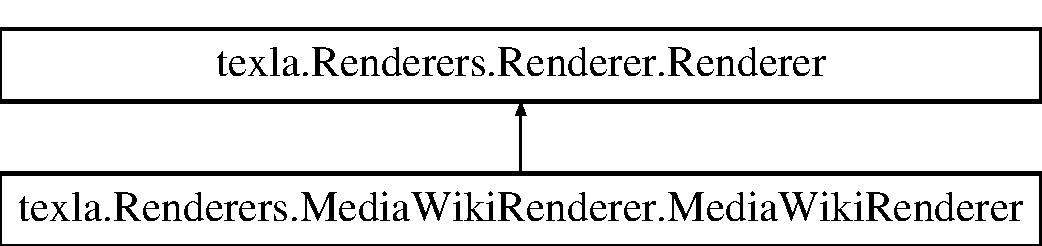
\includegraphics[height=2.000000cm]{classtexla_1_1Renderers_1_1MediaWikiRenderer_1_1MediaWikiRenderer}
\end{center}
\end{figure}
\subsection*{Public Member Functions}
\begin{DoxyCompactItemize}
\item 
\hypertarget{classtexla_1_1Renderers_1_1MediaWikiRenderer_1_1MediaWikiRenderer_ace84e554bf341a2cdb908e7268a04b7b}{}\label{classtexla_1_1Renderers_1_1MediaWikiRenderer_1_1MediaWikiRenderer_ace84e554bf341a2cdb908e7268a04b7b} 
def {\bfseries \+\_\+\+\_\+init\+\_\+\+\_\+} (self, configs)
\item 
def \hyperlink{classtexla_1_1Renderers_1_1MediaWikiRenderer_1_1MediaWikiRenderer_a1f90d864abf95f0d477a699602dd9f32}{start\+\_\+rendering} (self, root\+\_\+block)
\begin{DoxyCompactList}\small\item\em S\+T\+A\+R\+T\+I\+NG P\+O\+I\+NT. \end{DoxyCompactList}\item 
\hypertarget{classtexla_1_1Renderers_1_1MediaWikiRenderer_1_1MediaWikiRenderer_aad3ae964a950d89ce639d553a230149d}{}\label{classtexla_1_1Renderers_1_1MediaWikiRenderer_1_1MediaWikiRenderer_aad3ae964a950d89ce639d553a230149d} 
def \hyperlink{classtexla_1_1Renderers_1_1MediaWikiRenderer_1_1MediaWikiRenderer_aad3ae964a950d89ce639d553a230149d}{r\+\_\+document} (self, block)
\begin{DoxyCompactList}\small\item\em R\+O\+OT B\+L\+O\+CK. \end{DoxyCompactList}\item 
\hypertarget{classtexla_1_1Renderers_1_1MediaWikiRenderer_1_1MediaWikiRenderer_a45f7715817730de0df9be9ad316a68cb}{}\label{classtexla_1_1Renderers_1_1MediaWikiRenderer_1_1MediaWikiRenderer_a45f7715817730de0df9be9ad316a68cb} 
def \hyperlink{classtexla_1_1Renderers_1_1MediaWikiRenderer_1_1MediaWikiRenderer_a45f7715817730de0df9be9ad316a68cb}{default} (self, block)
\begin{DoxyCompactList}\small\item\em D\+E\+F\+A\+U\+LT. \end{DoxyCompactList}\item 
\hypertarget{classtexla_1_1Renderers_1_1MediaWikiRenderer_1_1MediaWikiRenderer_aebc8e8567cd7c4bf47a58234c8501a32}{}\label{classtexla_1_1Renderers_1_1MediaWikiRenderer_1_1MediaWikiRenderer_aebc8e8567cd7c4bf47a58234c8501a32} 
def \hyperlink{classtexla_1_1Renderers_1_1MediaWikiRenderer_1_1MediaWikiRenderer_aebc8e8567cd7c4bf47a58234c8501a32}{r\+\_\+text} (self, block)
\begin{DoxyCompactList}\small\item\em T\+E\+XT. \end{DoxyCompactList}\item 
\hypertarget{classtexla_1_1Renderers_1_1MediaWikiRenderer_1_1MediaWikiRenderer_a26cbb9c963153fbc3eb1f3beb08e1885}{}\label{classtexla_1_1Renderers_1_1MediaWikiRenderer_1_1MediaWikiRenderer_a26cbb9c963153fbc3eb1f3beb08e1885} 
def {\bfseries r\+\_\+newline} (self, block)
\item 
\hypertarget{classtexla_1_1Renderers_1_1MediaWikiRenderer_1_1MediaWikiRenderer_a47cbd0c83b97130a59f225560a281058}{}\label{classtexla_1_1Renderers_1_1MediaWikiRenderer_1_1MediaWikiRenderer_a47cbd0c83b97130a59f225560a281058} 
def {\bfseries r\+\_\+newpage} (self, block)
\item 
\hypertarget{classtexla_1_1Renderers_1_1MediaWikiRenderer_1_1MediaWikiRenderer_a883f4fbf6f57e8f7e573f34b18d457ab}{}\label{classtexla_1_1Renderers_1_1MediaWikiRenderer_1_1MediaWikiRenderer_a883f4fbf6f57e8f7e573f34b18d457ab} 
def {\bfseries r\+\_\+par} (self, block)
\item 
\hypertarget{classtexla_1_1Renderers_1_1MediaWikiRenderer_1_1MediaWikiRenderer_ad8c4ebd410183268e03085dcb433037e}{}\label{classtexla_1_1Renderers_1_1MediaWikiRenderer_1_1MediaWikiRenderer_ad8c4ebd410183268e03085dcb433037e} 
def \hyperlink{classtexla_1_1Renderers_1_1MediaWikiRenderer_1_1MediaWikiRenderer_ad8c4ebd410183268e03085dcb433037e}{sectioning} (self, block)
\begin{DoxyCompactList}\small\item\em S\+E\+C\+T\+I\+O\+N\+I\+NG. \end{DoxyCompactList}\item 
\hypertarget{classtexla_1_1Renderers_1_1MediaWikiRenderer_1_1MediaWikiRenderer_a65e5a7878ac5284c130488825b41d517}{}\label{classtexla_1_1Renderers_1_1MediaWikiRenderer_1_1MediaWikiRenderer_a65e5a7878ac5284c130488825b41d517} 
def \hyperlink{classtexla_1_1Renderers_1_1MediaWikiRenderer_1_1MediaWikiRenderer_a65e5a7878ac5284c130488825b41d517}{r\+\_\+display\+\_\+math} (self, block)
\begin{DoxyCompactList}\small\item\em M\+A\+TH. \end{DoxyCompactList}\item 
\hypertarget{classtexla_1_1Renderers_1_1MediaWikiRenderer_1_1MediaWikiRenderer_ac4226e8e1112f5e79bfd27d35fe4c527}{}\label{classtexla_1_1Renderers_1_1MediaWikiRenderer_1_1MediaWikiRenderer_ac4226e8e1112f5e79bfd27d35fe4c527} 
def {\bfseries r\+\_\+inline\+\_\+math} (self, block)
\item 
\hypertarget{classtexla_1_1Renderers_1_1MediaWikiRenderer_1_1MediaWikiRenderer_ab9923a538349f3c3f2420ba5d47f8ddb}{}\label{classtexla_1_1Renderers_1_1MediaWikiRenderer_1_1MediaWikiRenderer_ab9923a538349f3c3f2420ba5d47f8ddb} 
def {\bfseries r\+\_\+align} (self, block)
\item 
\hypertarget{classtexla_1_1Renderers_1_1MediaWikiRenderer_1_1MediaWikiRenderer_aaf6a12ea7a761834d34a14dba912d2a7}{}\label{classtexla_1_1Renderers_1_1MediaWikiRenderer_1_1MediaWikiRenderer_aaf6a12ea7a761834d34a14dba912d2a7} 
def {\bfseries r\+\_\+gather} (self, block)
\item 
\hypertarget{classtexla_1_1Renderers_1_1MediaWikiRenderer_1_1MediaWikiRenderer_abed3062c10cda57471c71cd75334f3a1}{}\label{classtexla_1_1Renderers_1_1MediaWikiRenderer_1_1MediaWikiRenderer_abed3062c10cda57471c71cd75334f3a1} 
def \hyperlink{classtexla_1_1Renderers_1_1MediaWikiRenderer_1_1MediaWikiRenderer_abed3062c10cda57471c71cd75334f3a1}{r\+\_\+label} (self, block)
\begin{DoxyCompactList}\small\item\em L\+A\+B\+E\+LS and refs. \end{DoxyCompactList}\item 
\hypertarget{classtexla_1_1Renderers_1_1MediaWikiRenderer_1_1MediaWikiRenderer_a6a8584cbd3a1f80ac452f6769676af53}{}\label{classtexla_1_1Renderers_1_1MediaWikiRenderer_1_1MediaWikiRenderer_a6a8584cbd3a1f80ac452f6769676af53} 
def {\bfseries r\+\_\+ref} (self, block)
\item 
\hypertarget{classtexla_1_1Renderers_1_1MediaWikiRenderer_1_1MediaWikiRenderer_acbd001b49a49d2952ce581202a10d8d3}{}\label{classtexla_1_1Renderers_1_1MediaWikiRenderer_1_1MediaWikiRenderer_acbd001b49a49d2952ce581202a10d8d3} 
def \hyperlink{classtexla_1_1Renderers_1_1MediaWikiRenderer_1_1MediaWikiRenderer_acbd001b49a49d2952ce581202a10d8d3}{r\+\_\+special\+\_\+character} (self, block)
\begin{DoxyCompactList}\small\item\em F\+O\+R\+M\+A\+T\+T\+I\+NG. \end{DoxyCompactList}\item 
\hypertarget{classtexla_1_1Renderers_1_1MediaWikiRenderer_1_1MediaWikiRenderer_a02e4f5e87a2bb4d22e3e5f84839ddee6}{}\label{classtexla_1_1Renderers_1_1MediaWikiRenderer_1_1MediaWikiRenderer_a02e4f5e87a2bb4d22e3e5f84839ddee6} 
def {\bfseries r\+\_\+dots} (self, block)
\item 
\hypertarget{classtexla_1_1Renderers_1_1MediaWikiRenderer_1_1MediaWikiRenderer_a1b8a95c6858e5885a52f94b2854bb54b}{}\label{classtexla_1_1Renderers_1_1MediaWikiRenderer_1_1MediaWikiRenderer_a1b8a95c6858e5885a52f94b2854bb54b} 
def {\bfseries r\+\_\+textbf} (self, block)
\item 
\hypertarget{classtexla_1_1Renderers_1_1MediaWikiRenderer_1_1MediaWikiRenderer_a0d4e83d75ad9a2868aeffc19b565a19e}{}\label{classtexla_1_1Renderers_1_1MediaWikiRenderer_1_1MediaWikiRenderer_a0d4e83d75ad9a2868aeffc19b565a19e} 
def {\bfseries r\+\_\+textit} (self, block)
\item 
\hypertarget{classtexla_1_1Renderers_1_1MediaWikiRenderer_1_1MediaWikiRenderer_a8eee2fceff70a4662e1e4505adc9d780}{}\label{classtexla_1_1Renderers_1_1MediaWikiRenderer_1_1MediaWikiRenderer_a8eee2fceff70a4662e1e4505adc9d780} 
def {\bfseries r\+\_\+textsc} (self, block)
\item 
\hypertarget{classtexla_1_1Renderers_1_1MediaWikiRenderer_1_1MediaWikiRenderer_af9c116742e58bccd97f80fbac7e72980}{}\label{classtexla_1_1Renderers_1_1MediaWikiRenderer_1_1MediaWikiRenderer_af9c116742e58bccd97f80fbac7e72980} 
def {\bfseries r\+\_\+superscript} (self, block)
\item 
\hypertarget{classtexla_1_1Renderers_1_1MediaWikiRenderer_1_1MediaWikiRenderer_acdfd0772b74a6309961a0d25b0e60b33}{}\label{classtexla_1_1Renderers_1_1MediaWikiRenderer_1_1MediaWikiRenderer_acdfd0772b74a6309961a0d25b0e60b33} 
def {\bfseries r\+\_\+subscript} (self, block)
\item 
\hypertarget{classtexla_1_1Renderers_1_1MediaWikiRenderer_1_1MediaWikiRenderer_a7620ace22f617a9cf31a824f8a117fb4}{}\label{classtexla_1_1Renderers_1_1MediaWikiRenderer_1_1MediaWikiRenderer_a7620ace22f617a9cf31a824f8a117fb4} 
def {\bfseries r\+\_\+underline} (self, block)
\item 
\hypertarget{classtexla_1_1Renderers_1_1MediaWikiRenderer_1_1MediaWikiRenderer_aeb2f92b5083008f825e27c550f0630aa}{}\label{classtexla_1_1Renderers_1_1MediaWikiRenderer_1_1MediaWikiRenderer_aeb2f92b5083008f825e27c550f0630aa} 
def {\bfseries r\+\_\+abstract} (self, block)
\item 
\hypertarget{classtexla_1_1Renderers_1_1MediaWikiRenderer_1_1MediaWikiRenderer_aebbc074a113d44f29e2904f418fd233c}{}\label{classtexla_1_1Renderers_1_1MediaWikiRenderer_1_1MediaWikiRenderer_aebbc074a113d44f29e2904f418fd233c} 
def {\bfseries r\+\_\+break} (self, block)
\item 
\hypertarget{classtexla_1_1Renderers_1_1MediaWikiRenderer_1_1MediaWikiRenderer_ab73aebbd6d392950e45908782fabaefe}{}\label{classtexla_1_1Renderers_1_1MediaWikiRenderer_1_1MediaWikiRenderer_ab73aebbd6d392950e45908782fabaefe} 
def {\bfseries r\+\_\+vspace} (self, block)
\item 
\hypertarget{classtexla_1_1Renderers_1_1MediaWikiRenderer_1_1MediaWikiRenderer_a881d4802011e7bb177b426080ef347ef}{}\label{classtexla_1_1Renderers_1_1MediaWikiRenderer_1_1MediaWikiRenderer_a881d4802011e7bb177b426080ef347ef} 
def {\bfseries r\+\_\+mandatory\+\_\+space} (self, block)
\item 
\hypertarget{classtexla_1_1Renderers_1_1MediaWikiRenderer_1_1MediaWikiRenderer_a376c11cdc8f476c1cd190f0529267305}{}\label{classtexla_1_1Renderers_1_1MediaWikiRenderer_1_1MediaWikiRenderer_a376c11cdc8f476c1cd190f0529267305} 
def {\bfseries r\+\_\+verbatim} (self, block)
\item 
\hypertarget{classtexla_1_1Renderers_1_1MediaWikiRenderer_1_1MediaWikiRenderer_ab69738e0d3102ca928d21773cedc64bc}{}\label{classtexla_1_1Renderers_1_1MediaWikiRenderer_1_1MediaWikiRenderer_ab69738e0d3102ca928d21773cedc64bc} 
def {\bfseries r\+\_\+verb} (self, block)
\item 
\hypertarget{classtexla_1_1Renderers_1_1MediaWikiRenderer_1_1MediaWikiRenderer_a2d7334f45d91f58e59cc26c9c7691c51}{}\label{classtexla_1_1Renderers_1_1MediaWikiRenderer_1_1MediaWikiRenderer_a2d7334f45d91f58e59cc26c9c7691c51} 
def \hyperlink{classtexla_1_1Renderers_1_1MediaWikiRenderer_1_1MediaWikiRenderer_a2d7334f45d91f58e59cc26c9c7691c51}{r\+\_\+center} (self, block)
\begin{DoxyCompactList}\small\item\em A\+L\+I\+G\+N\+M\+E\+NT. \end{DoxyCompactList}\item 
\hypertarget{classtexla_1_1Renderers_1_1MediaWikiRenderer_1_1MediaWikiRenderer_a4c2ae3ea597d159c48a2ee5b7fe22097}{}\label{classtexla_1_1Renderers_1_1MediaWikiRenderer_1_1MediaWikiRenderer_a4c2ae3ea597d159c48a2ee5b7fe22097} 
def {\bfseries r\+\_\+flushleft} (self, block)
\item 
\hypertarget{classtexla_1_1Renderers_1_1MediaWikiRenderer_1_1MediaWikiRenderer_a0505128514f3885a73832dcd99a1a7c9}{}\label{classtexla_1_1Renderers_1_1MediaWikiRenderer_1_1MediaWikiRenderer_a0505128514f3885a73832dcd99a1a7c9} 
def {\bfseries r\+\_\+flushright} (self, block)
\item 
\hypertarget{classtexla_1_1Renderers_1_1MediaWikiRenderer_1_1MediaWikiRenderer_a212b3b310e6bdcd83b9a75e7be96f62e}{}\label{classtexla_1_1Renderers_1_1MediaWikiRenderer_1_1MediaWikiRenderer_a212b3b310e6bdcd83b9a75e7be96f62e} 
def \hyperlink{classtexla_1_1Renderers_1_1MediaWikiRenderer_1_1MediaWikiRenderer_a212b3b310e6bdcd83b9a75e7be96f62e}{r\+\_\+itemize} (self, block)
\begin{DoxyCompactList}\small\item\em L\+I\+S\+TS. \end{DoxyCompactList}\item 
\hypertarget{classtexla_1_1Renderers_1_1MediaWikiRenderer_1_1MediaWikiRenderer_afde7519b22f693f0cdc97a6e2edc973e}{}\label{classtexla_1_1Renderers_1_1MediaWikiRenderer_1_1MediaWikiRenderer_afde7519b22f693f0cdc97a6e2edc973e} 
def {\bfseries r\+\_\+enumerate} (self, block)
\item 
\hypertarget{classtexla_1_1Renderers_1_1MediaWikiRenderer_1_1MediaWikiRenderer_ac629f74093d252426c108e760d92ae20}{}\label{classtexla_1_1Renderers_1_1MediaWikiRenderer_1_1MediaWikiRenderer_ac629f74093d252426c108e760d92ae20} 
def {\bfseries r\+\_\+description} (self, block)
\item 
\hypertarget{classtexla_1_1Renderers_1_1MediaWikiRenderer_1_1MediaWikiRenderer_a91b95087ac714d9378b5d085baa56a46}{}\label{classtexla_1_1Renderers_1_1MediaWikiRenderer_1_1MediaWikiRenderer_a91b95087ac714d9378b5d085baa56a46} 
def \hyperlink{classtexla_1_1Renderers_1_1MediaWikiRenderer_1_1MediaWikiRenderer_a91b95087ac714d9378b5d085baa56a46}{r\+\_\+quotes} (self, block)
\begin{DoxyCompactList}\small\item\em Q\+U\+O\+T\+ES. \end{DoxyCompactList}\item 
\hypertarget{classtexla_1_1Renderers_1_1MediaWikiRenderer_1_1MediaWikiRenderer_a4362cd2d5fc8ee30f6f9b1e6228b6d8e}{}\label{classtexla_1_1Renderers_1_1MediaWikiRenderer_1_1MediaWikiRenderer_a4362cd2d5fc8ee30f6f9b1e6228b6d8e} 
def {\bfseries r\+\_\+verse} (self, block)
\item 
\hypertarget{classtexla_1_1Renderers_1_1MediaWikiRenderer_1_1MediaWikiRenderer_ad6c163622d0e237789ba8a51539c1b97}{}\label{classtexla_1_1Renderers_1_1MediaWikiRenderer_1_1MediaWikiRenderer_ad6c163622d0e237789ba8a51539c1b97} 
def {\bfseries r\+\_\+footnote} (self, block)
\item 
\hypertarget{classtexla_1_1Renderers_1_1MediaWikiRenderer_1_1MediaWikiRenderer_a26753ab97b969c1590f4e7b3d380704c}{}\label{classtexla_1_1Renderers_1_1MediaWikiRenderer_1_1MediaWikiRenderer_a26753ab97b969c1590f4e7b3d380704c} 
def \hyperlink{classtexla_1_1Renderers_1_1MediaWikiRenderer_1_1MediaWikiRenderer_a26753ab97b969c1590f4e7b3d380704c}{r\+\_\+theorem} (self, block)
\begin{DoxyCompactList}\small\item\em Theorems. \end{DoxyCompactList}\item 
\hypertarget{classtexla_1_1Renderers_1_1MediaWikiRenderer_1_1MediaWikiRenderer_ab2150e20413c53eecf92b9106cde67ed}{}\label{classtexla_1_1Renderers_1_1MediaWikiRenderer_1_1MediaWikiRenderer_ab2150e20413c53eecf92b9106cde67ed} 
def {\bfseries r\+\_\+proof} (self, block)
\item 
\hypertarget{classtexla_1_1Renderers_1_1MediaWikiRenderer_1_1MediaWikiRenderer_adce08a943725c7ca5d5a559d59211c46}{}\label{classtexla_1_1Renderers_1_1MediaWikiRenderer_1_1MediaWikiRenderer_adce08a943725c7ca5d5a559d59211c46} 
def \hyperlink{classtexla_1_1Renderers_1_1MediaWikiRenderer_1_1MediaWikiRenderer_adce08a943725c7ca5d5a559d59211c46}{r\+\_\+accented\+\_\+letter} (self, block)
\begin{DoxyCompactList}\small\item\em A\+C\+C\+E\+N\+T\+ED letters. \end{DoxyCompactList}\end{DoxyCompactItemize}
\subsection*{Public Attributes}
\begin{DoxyCompactItemize}
\item 
\hypertarget{classtexla_1_1Renderers_1_1MediaWikiRenderer_1_1MediaWikiRenderer_a21d6343fcfb77695f189c0ae8bb1431c}{}\label{classtexla_1_1Renderers_1_1MediaWikiRenderer_1_1MediaWikiRenderer_a21d6343fcfb77695f189c0ae8bb1431c} 
{\bfseries configs}
\item 
\hypertarget{classtexla_1_1Renderers_1_1MediaWikiRenderer_1_1MediaWikiRenderer_ab2d0bab281d0bf9cf290c07eed6cb4de}{}\label{classtexla_1_1Renderers_1_1MediaWikiRenderer_1_1MediaWikiRenderer_ab2d0bab281d0bf9cf290c07eed6cb4de} 
{\bfseries doc\+\_\+title}
\item 
\hypertarget{classtexla_1_1Renderers_1_1MediaWikiRenderer_1_1MediaWikiRenderer_a3b844993ae27ebdab4ba8433276bd578}{}\label{classtexla_1_1Renderers_1_1MediaWikiRenderer_1_1MediaWikiRenderer_a3b844993ae27ebdab4ba8433276bd578} 
{\bfseries render\+\_\+hooks}
\item 
\hypertarget{classtexla_1_1Renderers_1_1MediaWikiRenderer_1_1MediaWikiRenderer_a9aa63e120fc85a9a30becb0b4ee7d895}{}\label{classtexla_1_1Renderers_1_1MediaWikiRenderer_1_1MediaWikiRenderer_a9aa63e120fc85a9a30becb0b4ee7d895} 
{\bfseries tree}
\item 
\hypertarget{classtexla_1_1Renderers_1_1MediaWikiRenderer_1_1MediaWikiRenderer_ab1f067192ea278cb00b863aac3450e01}{}\label{classtexla_1_1Renderers_1_1MediaWikiRenderer_1_1MediaWikiRenderer_ab1f067192ea278cb00b863aac3450e01} 
{\bfseries list\+\_\+level}
\item 
\hypertarget{classtexla_1_1Renderers_1_1MediaWikiRenderer_1_1MediaWikiRenderer_a4884a91fb1e345ed78ca25eed0bed3b6}{}\label{classtexla_1_1Renderers_1_1MediaWikiRenderer_1_1MediaWikiRenderer_a4884a91fb1e345ed78ca25eed0bed3b6} 
{\bfseries in\+\_\+theorem}
\item 
\hypertarget{classtexla_1_1Renderers_1_1MediaWikiRenderer_1_1MediaWikiRenderer_af527272b3eae4649046782080907f351}{}\label{classtexla_1_1Renderers_1_1MediaWikiRenderer_1_1MediaWikiRenderer_af527272b3eae4649046782080907f351} 
{\bfseries theorem\+\_\+number}
\item 
\hypertarget{classtexla_1_1Renderers_1_1MediaWikiRenderer_1_1MediaWikiRenderer_a4d28d8888ba967f2d6d8f7d9779f9a01}{}\label{classtexla_1_1Renderers_1_1MediaWikiRenderer_1_1MediaWikiRenderer_a4d28d8888ba967f2d6d8f7d9779f9a01} 
{\bfseries th\+\_\+numbering}
\end{DoxyCompactItemize}


\subsection{Member Function Documentation}
\hypertarget{classtexla_1_1Renderers_1_1MediaWikiRenderer_1_1MediaWikiRenderer_a1f90d864abf95f0d477a699602dd9f32}{}\label{classtexla_1_1Renderers_1_1MediaWikiRenderer_1_1MediaWikiRenderer_a1f90d864abf95f0d477a699602dd9f32} 
\index{texla\+::\+Renderers\+::\+Media\+Wiki\+Renderer\+::\+Media\+Wiki\+Renderer@{texla\+::\+Renderers\+::\+Media\+Wiki\+Renderer\+::\+Media\+Wiki\+Renderer}!start\+\_\+rendering@{start\+\_\+rendering}}
\index{start\+\_\+rendering@{start\+\_\+rendering}!texla\+::\+Renderers\+::\+Media\+Wiki\+Renderer\+::\+Media\+Wiki\+Renderer@{texla\+::\+Renderers\+::\+Media\+Wiki\+Renderer\+::\+Media\+Wiki\+Renderer}}
\subsubsection{\texorpdfstring{start\+\_\+rendering()}{start\_rendering()}}
{\footnotesize\ttfamily def texla.\+Renderers.\+Media\+Wiki\+Renderer.\+Media\+Wiki\+Renderer.\+start\+\_\+rendering (\begin{DoxyParamCaption}\item[{}]{self,  }\item[{}]{root\+\_\+block }\end{DoxyParamCaption})}



S\+T\+A\+R\+T\+I\+NG P\+O\+I\+NT. 

\begin{DoxyVerb}starting rendering from root-block\end{DoxyVerb}
 

The documentation for this class was generated from the following file\+:\begin{DoxyCompactItemize}
\item 
texla/\+Renderers/Media\+Wiki\+Renderer.\+py\end{DoxyCompactItemize}

\hypertarget{classtexla_1_1Parser_1_1Blocks_1_1BreakBlocks_1_1NewlineBlock}{}\section{texla.\+Parser.\+Blocks.\+Break\+Blocks.\+Newline\+Block Class Reference}
\label{classtexla_1_1Parser_1_1Blocks_1_1BreakBlocks_1_1NewlineBlock}\index{texla.\+Parser.\+Blocks.\+Break\+Blocks.\+Newline\+Block@{texla.\+Parser.\+Blocks.\+Break\+Blocks.\+Newline\+Block}}
Inheritance diagram for texla.\+Parser.\+Blocks.\+Break\+Blocks.\+Newline\+Block\+:\begin{figure}[H]
\begin{center}
\leavevmode
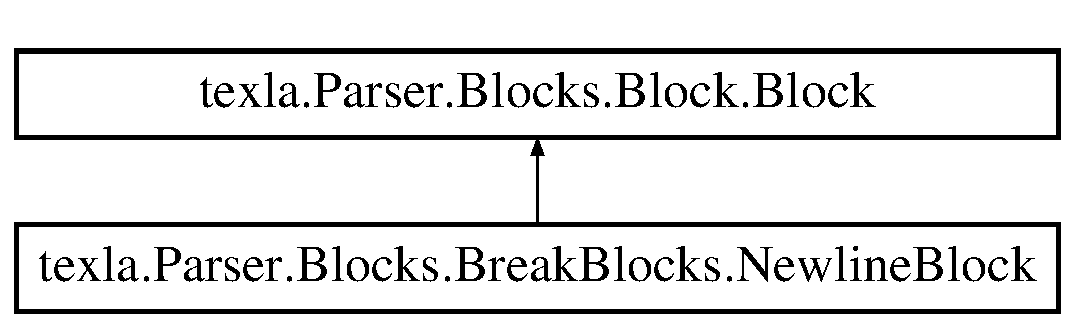
\includegraphics[height=2.000000cm]{classtexla_1_1Parser_1_1Blocks_1_1BreakBlocks_1_1NewlineBlock}
\end{center}
\end{figure}
\subsection*{Public Member Functions}
\begin{DoxyCompactItemize}
\item 
\hypertarget{classtexla_1_1Parser_1_1Blocks_1_1BreakBlocks_1_1NewlineBlock_a65d850875d25efcf16942abe2dc59901}{}\label{classtexla_1_1Parser_1_1Blocks_1_1BreakBlocks_1_1NewlineBlock_a65d850875d25efcf16942abe2dc59901} 
def {\bfseries parse\+\_\+newline} (parser, tex, parent\+\_\+block, params)
\item 
\hypertarget{classtexla_1_1Parser_1_1Blocks_1_1BreakBlocks_1_1NewlineBlock_af8b2345d33c08003c972d9c6852feea6}{}\label{classtexla_1_1Parser_1_1Blocks_1_1BreakBlocks_1_1NewlineBlock_af8b2345d33c08003c972d9c6852feea6} 
def {\bfseries \+\_\+\+\_\+init\+\_\+\+\_\+} (self, star, parent\+\_\+block)
\end{DoxyCompactItemize}
\subsection*{Additional Inherited Members}


The documentation for this class was generated from the following file\+:\begin{DoxyCompactItemize}
\item 
texla/\+Parser/\+Blocks/Break\+Blocks.\+py\end{DoxyCompactItemize}

\hypertarget{classtexla_1_1Parser_1_1Blocks_1_1BreakBlocks_1_1NewPageBlock}{}\section{texla.\+Parser.\+Blocks.\+Break\+Blocks.\+New\+Page\+Block Class Reference}
\label{classtexla_1_1Parser_1_1Blocks_1_1BreakBlocks_1_1NewPageBlock}\index{texla.\+Parser.\+Blocks.\+Break\+Blocks.\+New\+Page\+Block@{texla.\+Parser.\+Blocks.\+Break\+Blocks.\+New\+Page\+Block}}
Inheritance diagram for texla.\+Parser.\+Blocks.\+Break\+Blocks.\+New\+Page\+Block\+:\begin{figure}[H]
\begin{center}
\leavevmode
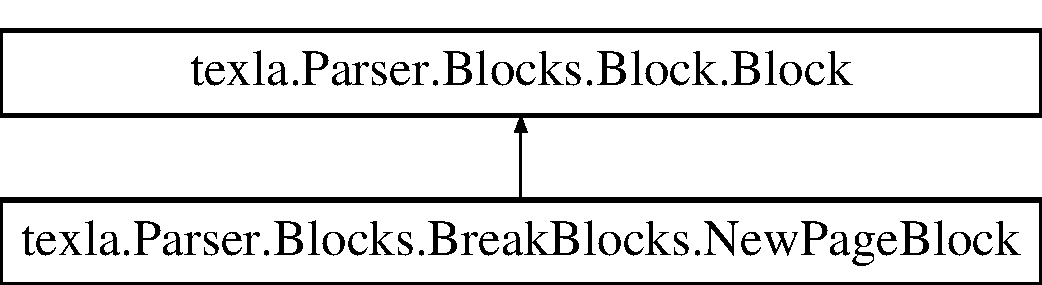
\includegraphics[height=2.000000cm]{classtexla_1_1Parser_1_1Blocks_1_1BreakBlocks_1_1NewPageBlock}
\end{center}
\end{figure}
\subsection*{Public Member Functions}
\begin{DoxyCompactItemize}
\item 
\hypertarget{classtexla_1_1Parser_1_1Blocks_1_1BreakBlocks_1_1NewPageBlock_a633148dfeab769b07555cab8287f37e0}{}\label{classtexla_1_1Parser_1_1Blocks_1_1BreakBlocks_1_1NewPageBlock_a633148dfeab769b07555cab8287f37e0} 
def {\bfseries \+\_\+\+\_\+init\+\_\+\+\_\+} (self, star, parent\+\_\+block)
\end{DoxyCompactItemize}
\subsection*{Static Public Member Functions}
\begin{DoxyCompactItemize}
\item 
\hypertarget{classtexla_1_1Parser_1_1Blocks_1_1BreakBlocks_1_1NewPageBlock_ac4bd36c82dcc09def4bb12fe12766455}{}\label{classtexla_1_1Parser_1_1Blocks_1_1BreakBlocks_1_1NewPageBlock_ac4bd36c82dcc09def4bb12fe12766455} 
def {\bfseries parse\+\_\+newpage} (parser, tex, parent\+\_\+block, params)
\end{DoxyCompactItemize}
\subsection*{Additional Inherited Members}


The documentation for this class was generated from the following file\+:\begin{DoxyCompactItemize}
\item 
texla/\+Parser/\+Blocks/Break\+Blocks.\+py\end{DoxyCompactItemize}

\hypertarget{classtexla_1_1Parser_1_1Blocks_1_1NoOptCommandBlock_1_1NoOptCommandBlock}{}\section{texla.\+Parser.\+Blocks.\+No\+Opt\+Command\+Block.\+No\+Opt\+Command\+Block Class Reference}
\label{classtexla_1_1Parser_1_1Blocks_1_1NoOptCommandBlock_1_1NoOptCommandBlock}\index{texla.\+Parser.\+Blocks.\+No\+Opt\+Command\+Block.\+No\+Opt\+Command\+Block@{texla.\+Parser.\+Blocks.\+No\+Opt\+Command\+Block.\+No\+Opt\+Command\+Block}}
Inheritance diagram for texla.\+Parser.\+Blocks.\+No\+Opt\+Command\+Block.\+No\+Opt\+Command\+Block\+:\begin{figure}[H]
\begin{center}
\leavevmode
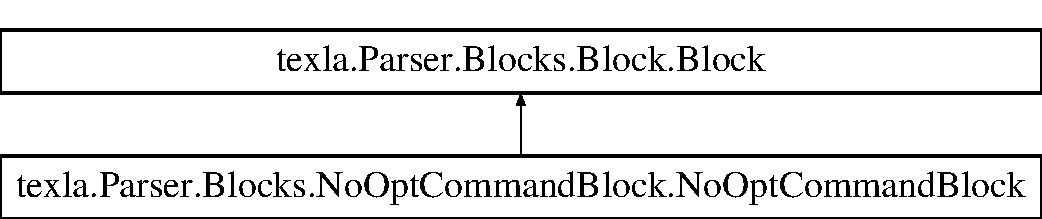
\includegraphics[height=2.000000cm]{classtexla_1_1Parser_1_1Blocks_1_1NoOptCommandBlock_1_1NoOptCommandBlock}
\end{center}
\end{figure}
\subsection*{Public Member Functions}
\begin{DoxyCompactItemize}
\item 
\hypertarget{classtexla_1_1Parser_1_1Blocks_1_1NoOptCommandBlock_1_1NoOptCommandBlock_aac0e7414e74ce9f20f7a9e35a9beb990}{}\label{classtexla_1_1Parser_1_1Blocks_1_1NoOptCommandBlock_1_1NoOptCommandBlock_aac0e7414e74ce9f20f7a9e35a9beb990} 
def {\bfseries \+\_\+\+\_\+init\+\_\+\+\_\+} (self, block\+\_\+name, star, parent\+\_\+block)
\end{DoxyCompactItemize}
\subsection*{Static Public Member Functions}
\begin{DoxyCompactItemize}
\item 
\hypertarget{classtexla_1_1Parser_1_1Blocks_1_1NoOptCommandBlock_1_1NoOptCommandBlock_a5be4dbd0ca161ab2a3707ea5e3ce2fb4}{}\label{classtexla_1_1Parser_1_1Blocks_1_1NoOptCommandBlock_1_1NoOptCommandBlock_a5be4dbd0ca161ab2a3707ea5e3ce2fb4} 
def {\bfseries parse} (parser, tex, parent\+\_\+block, params)
\end{DoxyCompactItemize}
\subsection*{Additional Inherited Members}


\subsection{Detailed Description}
\begin{DoxyVerb}This class is for generic commands without options\end{DoxyVerb}
 

The documentation for this class was generated from the following file\+:\begin{DoxyCompactItemize}
\item 
texla/\+Parser/\+Blocks/No\+Opt\+Command\+Block.\+py\end{DoxyCompactItemize}

\hypertarget{classtexla_1_1PageTree_1_1Page_1_1Page}{}\section{texla.\+Page\+Tree.\+Page.\+Page Class Reference}
\label{classtexla_1_1PageTree_1_1Page_1_1Page}\index{texla.\+Page\+Tree.\+Page.\+Page@{texla.\+Page\+Tree.\+Page.\+Page}}
\subsection*{Public Member Functions}
\begin{DoxyCompactItemize}
\item 
\hypertarget{classtexla_1_1PageTree_1_1Page_1_1Page_a5590937851fd4176e0ed6d6b27904bbc}{}\label{classtexla_1_1PageTree_1_1Page_1_1Page_a5590937851fd4176e0ed6d6b27904bbc} 
def {\bfseries \+\_\+\+\_\+init\+\_\+\+\_\+} (self, title, page\+\_\+type, level, keywords)
\item 
\hypertarget{classtexla_1_1PageTree_1_1Page_1_1Page_a67eeb89e1b0fb3cf5e98d3f734d468ea}{}\label{classtexla_1_1PageTree_1_1Page_1_1Page_a67eeb89e1b0fb3cf5e98d3f734d468ea} 
def {\bfseries add\+Text} (self, text)
\item 
def \hyperlink{classtexla_1_1PageTree_1_1Page_1_1Page_a2c10bde17648f6c1c4d0ddfba6300a62}{add\+Subpage} (self, page, after=None)
\item 
def \hyperlink{classtexla_1_1PageTree_1_1Page_1_1Page_a040ae3dde5163b524191b66e91c3f80e}{add\+Subpages} (self, pages, after=None)
\item 
def \hyperlink{classtexla_1_1PageTree_1_1Page_1_1Page_ad9d4ce2ebe5586474919d5e5e9d1eac8}{add\+Subpage\+\_\+top} (self, page)
\item 
def \hyperlink{classtexla_1_1PageTree_1_1Page_1_1Page_a6c977d8a5d051a28520de3f2bf5f17ee}{remove\+Subpage} (self, page)
\item 
\hypertarget{classtexla_1_1PageTree_1_1Page_1_1Page_a1d4e034af4d7f60c0110baf8324005c2}{}\label{classtexla_1_1PageTree_1_1Page_1_1Page_a1d4e034af4d7f60c0110baf8324005c2} 
def {\bfseries is\+Subpage} (self, page)
\item 
def \hyperlink{classtexla_1_1PageTree_1_1Page_1_1Page_a6d72f71ac5e2997ad4cc46857223081b}{get\+\_\+subpages} (self)
\item 
def \hyperlink{classtexla_1_1PageTree_1_1Page_1_1Page_aa16c3d6d8ec200fa8e4414d152e84577}{refresh\+\_\+level} (self, new\+\_\+level)
\item 
def \hyperlink{classtexla_1_1PageTree_1_1Page_1_1Page_a6c12e22fb2a28e4e64678b04f8a6e70c}{after\+\_\+render} (self)
\item 
def \hyperlink{classtexla_1_1PageTree_1_1Page_1_1Page_a6d435028bd474b1b36abdbd4387fd08f}{collapse\+Subpages\+Text} (self, level=0)
\item 
def \hyperlink{classtexla_1_1PageTree_1_1Page_1_1Page_ab9d5fa24adb9159e80a0e5253f501622}{collapse\+U\+RL} (self, base\+\_\+url)
\item 
def \hyperlink{classtexla_1_1PageTree_1_1Page_1_1Page_a4c813de1c404e86c8e55c73e017ad4b2}{create\+\_\+pagenumbers} (self, parent, current)
\item 
def \hyperlink{classtexla_1_1PageTree_1_1Page_1_1Page_aac15419ccf4b4ca1d50dc91dc2fc8e20}{fix\+\_\+text\+\_\+characters} (self)
\item 
def \hyperlink{classtexla_1_1PageTree_1_1Page_1_1Page_a83054589cb1c1f29959693ac9ab8fd93}{is\+\_\+math\+\_\+inside\+\_\+title} (self)
\item 
def \hyperlink{classtexla_1_1PageTree_1_1Page_1_1Page_a2a63bd250b119f66631c4129ed982093}{get\+\_\+json\+\_\+dictionary} (self, pages)
\item 
\hypertarget{classtexla_1_1PageTree_1_1Page_1_1Page_ad67d6552dd5d4e781fe823b059d2aa78}{}\label{classtexla_1_1PageTree_1_1Page_1_1Page_ad67d6552dd5d4e781fe823b059d2aa78} 
def {\bfseries get\+\_\+str} (self)
\item 
\hypertarget{classtexla_1_1PageTree_1_1Page_1_1Page_a43f3989a712c7ae3101c96bc7753874b}{}\label{classtexla_1_1PageTree_1_1Page_1_1Page_a43f3989a712c7ae3101c96bc7753874b} 
def {\bfseries \+\_\+\+\_\+str\+\_\+\+\_\+} (self)
\end{DoxyCompactItemize}
\subsection*{Public Attributes}
\begin{DoxyCompactItemize}
\item 
\hypertarget{classtexla_1_1PageTree_1_1Page_1_1Page_a8c9d762e50a5459766ef442faaf18473}{}\label{classtexla_1_1PageTree_1_1Page_1_1Page_a8c9d762e50a5459766ef442faaf18473} 
{\bfseries id}
\item 
\hypertarget{classtexla_1_1PageTree_1_1Page_1_1Page_ad6235d4f93ee98ea03075bcd7413c3e2}{}\label{classtexla_1_1PageTree_1_1Page_1_1Page_ad6235d4f93ee98ea03075bcd7413c3e2} 
{\bfseries title}
\item 
\hypertarget{classtexla_1_1PageTree_1_1Page_1_1Page_a0ee67f8aa35814848d1feaeb3dc819fd}{}\label{classtexla_1_1PageTree_1_1Page_1_1Page_a0ee67f8aa35814848d1feaeb3dc819fd} 
{\bfseries type}
\item 
\hypertarget{classtexla_1_1PageTree_1_1Page_1_1Page_a89d33cd5f6f28ce050453d716b5db156}{}\label{classtexla_1_1PageTree_1_1Page_1_1Page_a89d33cd5f6f28ce050453d716b5db156} 
{\bfseries keywords}
\item 
\hypertarget{classtexla_1_1PageTree_1_1Page_1_1Page_a6e390d41935444839e3511e1686415af}{}\label{classtexla_1_1PageTree_1_1Page_1_1Page_a6e390d41935444839e3511e1686415af} 
{\bfseries text}
\item 
\hypertarget{classtexla_1_1PageTree_1_1Page_1_1Page_af2a5faebed0cc6cd40708cc08ce606df}{}\label{classtexla_1_1PageTree_1_1Page_1_1Page_af2a5faebed0cc6cd40708cc08ce606df} 
{\bfseries collapsed}
\item 
\hypertarget{classtexla_1_1PageTree_1_1Page_1_1Page_a20ecd89a8c205dd433cef2e3bcedfd25}{}\label{classtexla_1_1PageTree_1_1Page_1_1Page_a20ecd89a8c205dd433cef2e3bcedfd25} 
{\bfseries subpages}
\item 
\hypertarget{classtexla_1_1PageTree_1_1Page_1_1Page_a79e0ed8249cdf553336f884d3a4d4b0f}{}\label{classtexla_1_1PageTree_1_1Page_1_1Page_a79e0ed8249cdf553336f884d3a4d4b0f} 
{\bfseries parent}
\item 
\hypertarget{classtexla_1_1PageTree_1_1Page_1_1Page_a1665eef742f953a65133cfc683434adb}{}\label{classtexla_1_1PageTree_1_1Page_1_1Page_a1665eef742f953a65133cfc683434adb} 
{\bfseries level}
\item 
\hypertarget{classtexla_1_1PageTree_1_1Page_1_1Page_a15139f62e61518b593b30e668ec0c0ce}{}\label{classtexla_1_1PageTree_1_1Page_1_1Page_a15139f62e61518b593b30e668ec0c0ce} 
{\bfseries math\+\_\+inside\+\_\+title}
\item 
\hypertarget{classtexla_1_1PageTree_1_1Page_1_1Page_a4381b56e123ad7db897a5d9062ea684c}{}\label{classtexla_1_1PageTree_1_1Page_1_1Page_a4381b56e123ad7db897a5d9062ea684c} 
{\bfseries url}
\item 
\hypertarget{classtexla_1_1PageTree_1_1Page_1_1Page_aa1289e341c0b73e7b14932b113cac264}{}\label{classtexla_1_1PageTree_1_1Page_1_1Page_aa1289e341c0b73e7b14932b113cac264} 
{\bfseries pagenumber}
\end{DoxyCompactItemize}


\subsection{Detailed Description}
\begin{DoxyVerb}Class that manages the pages content.
Data members of Page
-self.id = randon id of the page
-self.title is the title normalized for urls
-self.subpages contains the list of the subpages objects
-self.level memorize the level of the page.(root=-1))
-self.url contains the unique internal url of the page
-self.type is 'root',part,chapter,section,subsection,subsubection,paragraph.
-self.keywords is a dictionary with localized keywords for output\end{DoxyVerb}
 

\subsection{Member Function Documentation}
\hypertarget{classtexla_1_1PageTree_1_1Page_1_1Page_a2c10bde17648f6c1c4d0ddfba6300a62}{}\label{classtexla_1_1PageTree_1_1Page_1_1Page_a2c10bde17648f6c1c4d0ddfba6300a62} 
\index{texla\+::\+Page\+Tree\+::\+Page\+::\+Page@{texla\+::\+Page\+Tree\+::\+Page\+::\+Page}!add\+Subpage@{add\+Subpage}}
\index{add\+Subpage@{add\+Subpage}!texla\+::\+Page\+Tree\+::\+Page\+::\+Page@{texla\+::\+Page\+Tree\+::\+Page\+::\+Page}}
\subsubsection{\texorpdfstring{add\+Subpage()}{addSubpage()}}
{\footnotesize\ttfamily def texla.\+Page\+Tree.\+Page.\+Page.\+add\+Subpage (\begin{DoxyParamCaption}\item[{}]{self,  }\item[{}]{page,  }\item[{}]{after = {\ttfamily None} }\end{DoxyParamCaption})}

\begin{DoxyVerb}This methods add a subpage
refreshing the levels of ALL subpages.
It sets also the parent of the subpage\end{DoxyVerb}
 \hypertarget{classtexla_1_1PageTree_1_1Page_1_1Page_ad9d4ce2ebe5586474919d5e5e9d1eac8}{}\label{classtexla_1_1PageTree_1_1Page_1_1Page_ad9d4ce2ebe5586474919d5e5e9d1eac8} 
\index{texla\+::\+Page\+Tree\+::\+Page\+::\+Page@{texla\+::\+Page\+Tree\+::\+Page\+::\+Page}!add\+Subpage\+\_\+top@{add\+Subpage\+\_\+top}}
\index{add\+Subpage\+\_\+top@{add\+Subpage\+\_\+top}!texla\+::\+Page\+Tree\+::\+Page\+::\+Page@{texla\+::\+Page\+Tree\+::\+Page\+::\+Page}}
\subsubsection{\texorpdfstring{add\+Subpage\+\_\+top()}{addSubpage\_top()}}
{\footnotesize\ttfamily def texla.\+Page\+Tree.\+Page.\+Page.\+add\+Subpage\+\_\+top (\begin{DoxyParamCaption}\item[{}]{self,  }\item[{}]{page }\end{DoxyParamCaption})}

\begin{DoxyVerb}This function add a subpage before all the others.\end{DoxyVerb}
 \hypertarget{classtexla_1_1PageTree_1_1Page_1_1Page_a040ae3dde5163b524191b66e91c3f80e}{}\label{classtexla_1_1PageTree_1_1Page_1_1Page_a040ae3dde5163b524191b66e91c3f80e} 
\index{texla\+::\+Page\+Tree\+::\+Page\+::\+Page@{texla\+::\+Page\+Tree\+::\+Page\+::\+Page}!add\+Subpages@{add\+Subpages}}
\index{add\+Subpages@{add\+Subpages}!texla\+::\+Page\+Tree\+::\+Page\+::\+Page@{texla\+::\+Page\+Tree\+::\+Page\+::\+Page}}
\subsubsection{\texorpdfstring{add\+Subpages()}{addSubpages()}}
{\footnotesize\ttfamily def texla.\+Page\+Tree.\+Page.\+Page.\+add\+Subpages (\begin{DoxyParamCaption}\item[{}]{self,  }\item[{}]{pages,  }\item[{}]{after = {\ttfamily None} }\end{DoxyParamCaption})}

\begin{DoxyVerb}This function add a list of subpages,
setting levels and parent page.\end{DoxyVerb}
 \hypertarget{classtexla_1_1PageTree_1_1Page_1_1Page_a6c12e22fb2a28e4e64678b04f8a6e70c}{}\label{classtexla_1_1PageTree_1_1Page_1_1Page_a6c12e22fb2a28e4e64678b04f8a6e70c} 
\index{texla\+::\+Page\+Tree\+::\+Page\+::\+Page@{texla\+::\+Page\+Tree\+::\+Page\+::\+Page}!after\+\_\+render@{after\+\_\+render}}
\index{after\+\_\+render@{after\+\_\+render}!texla\+::\+Page\+Tree\+::\+Page\+::\+Page@{texla\+::\+Page\+Tree\+::\+Page\+::\+Page}}
\subsubsection{\texorpdfstring{after\+\_\+render()}{after\_render()}}
{\footnotesize\ttfamily def texla.\+Page\+Tree.\+Page.\+Page.\+after\+\_\+render (\begin{DoxyParamCaption}\item[{}]{self }\end{DoxyParamCaption})}

\begin{DoxyVerb}This function does some fixes after rendering\end{DoxyVerb}
 \hypertarget{classtexla_1_1PageTree_1_1Page_1_1Page_a6d435028bd474b1b36abdbd4387fd08f}{}\label{classtexla_1_1PageTree_1_1Page_1_1Page_a6d435028bd474b1b36abdbd4387fd08f} 
\index{texla\+::\+Page\+Tree\+::\+Page\+::\+Page@{texla\+::\+Page\+Tree\+::\+Page\+::\+Page}!collapse\+Subpages\+Text@{collapse\+Subpages\+Text}}
\index{collapse\+Subpages\+Text@{collapse\+Subpages\+Text}!texla\+::\+Page\+Tree\+::\+Page\+::\+Page@{texla\+::\+Page\+Tree\+::\+Page\+::\+Page}}
\subsubsection{\texorpdfstring{collapse\+Subpages\+Text()}{collapseSubpagesText()}}
{\footnotesize\ttfamily def texla.\+Page\+Tree.\+Page.\+Page.\+collapse\+Subpages\+Text (\begin{DoxyParamCaption}\item[{}]{self,  }\item[{}]{level = {\ttfamily 0} }\end{DoxyParamCaption})}

\begin{DoxyVerb}This method insert the text of subpages in this
page and returns the complete text.\end{DoxyVerb}
 \hypertarget{classtexla_1_1PageTree_1_1Page_1_1Page_ab9d5fa24adb9159e80a0e5253f501622}{}\label{classtexla_1_1PageTree_1_1Page_1_1Page_ab9d5fa24adb9159e80a0e5253f501622} 
\index{texla\+::\+Page\+Tree\+::\+Page\+::\+Page@{texla\+::\+Page\+Tree\+::\+Page\+::\+Page}!collapse\+U\+RL@{collapse\+U\+RL}}
\index{collapse\+U\+RL@{collapse\+U\+RL}!texla\+::\+Page\+Tree\+::\+Page\+::\+Page@{texla\+::\+Page\+Tree\+::\+Page\+::\+Page}}
\subsubsection{\texorpdfstring{collapse\+U\+R\+L()}{collapseURL()}}
{\footnotesize\ttfamily def texla.\+Page\+Tree.\+Page.\+Page.\+collapse\+U\+RL (\begin{DoxyParamCaption}\item[{}]{self,  }\item[{}]{base\+\_\+url }\end{DoxyParamCaption})}

\begin{DoxyVerb}This functions creates the url of the page
checking if it is collapsed. Then it continues
with the subpages\end{DoxyVerb}
 \hypertarget{classtexla_1_1PageTree_1_1Page_1_1Page_a4c813de1c404e86c8e55c73e017ad4b2}{}\label{classtexla_1_1PageTree_1_1Page_1_1Page_a4c813de1c404e86c8e55c73e017ad4b2} 
\index{texla\+::\+Page\+Tree\+::\+Page\+::\+Page@{texla\+::\+Page\+Tree\+::\+Page\+::\+Page}!create\+\_\+pagenumbers@{create\+\_\+pagenumbers}}
\index{create\+\_\+pagenumbers@{create\+\_\+pagenumbers}!texla\+::\+Page\+Tree\+::\+Page\+::\+Page@{texla\+::\+Page\+Tree\+::\+Page\+::\+Page}}
\subsubsection{\texorpdfstring{create\+\_\+pagenumbers()}{create\_pagenumbers()}}
{\footnotesize\ttfamily def texla.\+Page\+Tree.\+Page.\+Page.\+create\+\_\+pagenumbers (\begin{DoxyParamCaption}\item[{}]{self,  }\item[{}]{parent,  }\item[{}]{current }\end{DoxyParamCaption})}

\begin{DoxyVerb}This function creates the pagenumber string appending to the
parent number its position in the pages of the same level. Then
the process continues with subpages\end{DoxyVerb}
 \hypertarget{classtexla_1_1PageTree_1_1Page_1_1Page_aac15419ccf4b4ca1d50dc91dc2fc8e20}{}\label{classtexla_1_1PageTree_1_1Page_1_1Page_aac15419ccf4b4ca1d50dc91dc2fc8e20} 
\index{texla\+::\+Page\+Tree\+::\+Page\+::\+Page@{texla\+::\+Page\+Tree\+::\+Page\+::\+Page}!fix\+\_\+text\+\_\+characters@{fix\+\_\+text\+\_\+characters}}
\index{fix\+\_\+text\+\_\+characters@{fix\+\_\+text\+\_\+characters}!texla\+::\+Page\+Tree\+::\+Page\+::\+Page@{texla\+::\+Page\+Tree\+::\+Page\+::\+Page}}
\subsubsection{\texorpdfstring{fix\+\_\+text\+\_\+characters()}{fix\_text\_characters()}}
{\footnotesize\ttfamily def texla.\+Page\+Tree.\+Page.\+Page.\+fix\+\_\+text\+\_\+characters (\begin{DoxyParamCaption}\item[{}]{self }\end{DoxyParamCaption})}

\begin{DoxyVerb}Utility function to fix apostrophes and other characters
inside the text of the page\end{DoxyVerb}
 \hypertarget{classtexla_1_1PageTree_1_1Page_1_1Page_a2a63bd250b119f66631c4129ed982093}{}\label{classtexla_1_1PageTree_1_1Page_1_1Page_a2a63bd250b119f66631c4129ed982093} 
\index{texla\+::\+Page\+Tree\+::\+Page\+::\+Page@{texla\+::\+Page\+Tree\+::\+Page\+::\+Page}!get\+\_\+json\+\_\+dictionary@{get\+\_\+json\+\_\+dictionary}}
\index{get\+\_\+json\+\_\+dictionary@{get\+\_\+json\+\_\+dictionary}!texla\+::\+Page\+Tree\+::\+Page\+::\+Page@{texla\+::\+Page\+Tree\+::\+Page\+::\+Page}}
\subsubsection{\texorpdfstring{get\+\_\+json\+\_\+dictionary()}{get\_json\_dictionary()}}
{\footnotesize\ttfamily def texla.\+Page\+Tree.\+Page.\+Page.\+get\+\_\+json\+\_\+dictionary (\begin{DoxyParamCaption}\item[{}]{self,  }\item[{}]{pages }\end{DoxyParamCaption})}

\begin{DoxyVerb}This function return the json dictionary of the page
with all its children\end{DoxyVerb}
 \hypertarget{classtexla_1_1PageTree_1_1Page_1_1Page_a6d72f71ac5e2997ad4cc46857223081b}{}\label{classtexla_1_1PageTree_1_1Page_1_1Page_a6d72f71ac5e2997ad4cc46857223081b} 
\index{texla\+::\+Page\+Tree\+::\+Page\+::\+Page@{texla\+::\+Page\+Tree\+::\+Page\+::\+Page}!get\+\_\+subpages@{get\+\_\+subpages}}
\index{get\+\_\+subpages@{get\+\_\+subpages}!texla\+::\+Page\+Tree\+::\+Page\+::\+Page@{texla\+::\+Page\+Tree\+::\+Page\+::\+Page}}
\subsubsection{\texorpdfstring{get\+\_\+subpages()}{get\_subpages()}}
{\footnotesize\ttfamily def texla.\+Page\+Tree.\+Page.\+Page.\+get\+\_\+subpages (\begin{DoxyParamCaption}\item[{}]{self }\end{DoxyParamCaption})}

\begin{DoxyVerb}This function returns a list with all the subpages
of the current page walking the subtree
KEEPING THE ORDER (REALLY IMPORTANT):
-subpage:
    --subsub1
    --subsub2:
---subsubsub
-subpage2...
=> [subpage, subsub1, subsub2, subsubsub, subpage2, ...]\end{DoxyVerb}
 \hypertarget{classtexla_1_1PageTree_1_1Page_1_1Page_a83054589cb1c1f29959693ac9ab8fd93}{}\label{classtexla_1_1PageTree_1_1Page_1_1Page_a83054589cb1c1f29959693ac9ab8fd93} 
\index{texla\+::\+Page\+Tree\+::\+Page\+::\+Page@{texla\+::\+Page\+Tree\+::\+Page\+::\+Page}!is\+\_\+math\+\_\+inside\+\_\+title@{is\+\_\+math\+\_\+inside\+\_\+title}}
\index{is\+\_\+math\+\_\+inside\+\_\+title@{is\+\_\+math\+\_\+inside\+\_\+title}!texla\+::\+Page\+Tree\+::\+Page\+::\+Page@{texla\+::\+Page\+Tree\+::\+Page\+::\+Page}}
\subsubsection{\texorpdfstring{is\+\_\+math\+\_\+inside\+\_\+title()}{is\_math\_inside\_title()}}
{\footnotesize\ttfamily def texla.\+Page\+Tree.\+Page.\+Page.\+is\+\_\+math\+\_\+inside\+\_\+title (\begin{DoxyParamCaption}\item[{}]{self }\end{DoxyParamCaption})}

\begin{DoxyVerb}This function checkes if there is math inside titles\end{DoxyVerb}
 \hypertarget{classtexla_1_1PageTree_1_1Page_1_1Page_aa16c3d6d8ec200fa8e4414d152e84577}{}\label{classtexla_1_1PageTree_1_1Page_1_1Page_aa16c3d6d8ec200fa8e4414d152e84577} 
\index{texla\+::\+Page\+Tree\+::\+Page\+::\+Page@{texla\+::\+Page\+Tree\+::\+Page\+::\+Page}!refresh\+\_\+level@{refresh\+\_\+level}}
\index{refresh\+\_\+level@{refresh\+\_\+level}!texla\+::\+Page\+Tree\+::\+Page\+::\+Page@{texla\+::\+Page\+Tree\+::\+Page\+::\+Page}}
\subsubsection{\texorpdfstring{refresh\+\_\+level()}{refresh\_level()}}
{\footnotesize\ttfamily def texla.\+Page\+Tree.\+Page.\+Page.\+refresh\+\_\+level (\begin{DoxyParamCaption}\item[{}]{self,  }\item[{}]{new\+\_\+level }\end{DoxyParamCaption})}

\begin{DoxyVerb}This function change the level of this page
refreshing recursively all the subpages\end{DoxyVerb}
 \hypertarget{classtexla_1_1PageTree_1_1Page_1_1Page_a6c977d8a5d051a28520de3f2bf5f17ee}{}\label{classtexla_1_1PageTree_1_1Page_1_1Page_a6c977d8a5d051a28520de3f2bf5f17ee} 
\index{texla\+::\+Page\+Tree\+::\+Page\+::\+Page@{texla\+::\+Page\+Tree\+::\+Page\+::\+Page}!remove\+Subpage@{remove\+Subpage}}
\index{remove\+Subpage@{remove\+Subpage}!texla\+::\+Page\+Tree\+::\+Page\+::\+Page@{texla\+::\+Page\+Tree\+::\+Page\+::\+Page}}
\subsubsection{\texorpdfstring{remove\+Subpage()}{removeSubpage()}}
{\footnotesize\ttfamily def texla.\+Page\+Tree.\+Page.\+Page.\+remove\+Subpage (\begin{DoxyParamCaption}\item[{}]{self,  }\item[{}]{page }\end{DoxyParamCaption})}

\begin{DoxyVerb}This function removes the subpage
recursively looking also at subpages\end{DoxyVerb}
 

The documentation for this class was generated from the following file\+:\begin{DoxyCompactItemize}
\item 
texla/\+Page\+Tree/Page.\+py\end{DoxyCompactItemize}

\hypertarget{classtexla_1_1PageTree_1_1PageTree_1_1PageTree}{}\section{texla.\+Page\+Tree.\+Page\+Tree.\+Page\+Tree Class Reference}
\label{classtexla_1_1PageTree_1_1PageTree_1_1PageTree}\index{texla.\+Page\+Tree.\+Page\+Tree.\+Page\+Tree@{texla.\+Page\+Tree.\+Page\+Tree.\+Page\+Tree}}
\subsection*{Public Member Functions}
\begin{DoxyCompactItemize}
\item 
\hypertarget{classtexla_1_1PageTree_1_1PageTree_1_1PageTree_a163c567fb96bf817e560a5ceb37c9ccf}{}\label{classtexla_1_1PageTree_1_1PageTree_1_1PageTree_a163c567fb96bf817e560a5ceb37c9ccf} 
def {\bfseries \+\_\+\+\_\+init\+\_\+\+\_\+} (self, configs)
\item 
def \hyperlink{classtexla_1_1PageTree_1_1PageTree_1_1PageTree_a9df0c1cd2ebc4c0e0af693c49c084324}{create\+Page} (self, title, page\+\_\+type)
\item 
def \hyperlink{classtexla_1_1PageTree_1_1PageTree_1_1PageTree_adfd53d92c57eefb5d956cc1c3e646373}{exit\+Page} (self)
\item 
\hypertarget{classtexla_1_1PageTree_1_1PageTree_1_1PageTree_a1d56ecdff92229338afad2c7397c8010}{}\label{classtexla_1_1PageTree_1_1PageTree_1_1PageTree_a1d56ecdff92229338afad2c7397c8010} 
def {\bfseries add\+Text} (self, text)
\item 
def \hyperlink{classtexla_1_1PageTree_1_1PageTree_1_1PageTree_a7b0b920255477e1c0cf155147ded847a}{add\+Label} (self, label)
\item 
def \hyperlink{classtexla_1_1PageTree_1_1PageTree_1_1PageTree_ac5f3e4e6283924a193a513b2d9289c27}{add\+Reference} (self, label)
\item 
def \hyperlink{classtexla_1_1PageTree_1_1PageTree_1_1PageTree_ab34f6b054c920675e93f6e29694d54bf}{add\+Theorem} (self, id, th\+\_\+type)
\item 
def \hyperlink{classtexla_1_1PageTree_1_1PageTree_1_1PageTree_a6f720d497af55d8ccdeadb779d6a61bc}{exit\+Theorem} (self)
\item 
def \hyperlink{classtexla_1_1PageTree_1_1PageTree_1_1PageTree_aa01020f0c674d653538d819e6f1ca231}{get\+\_\+tree\+\_\+json} (self)
\item 
def \hyperlink{classtexla_1_1PageTree_1_1PageTree_1_1PageTree_ab6d7f8cb1defc5738cac8da13de74809}{get\+\_\+tree\+\_\+debug} (self)
\item 
def \hyperlink{classtexla_1_1PageTree_1_1PageTree_1_1PageTree_aef29edcb58ecab6f73b2fc00105bfd32}{after\+\_\+render} (self)
\item 
\hypertarget{classtexla_1_1PageTree_1_1PageTree_1_1PageTree_af00c05b145278ad8e9b4b67b9871ec28}{}\label{classtexla_1_1PageTree_1_1PageTree_1_1PageTree_af00c05b145278ad8e9b4b67b9871ec28} 
def {\bfseries change\+\_\+title} (self, page\+\_\+id, title)
\item 
def \hyperlink{classtexla_1_1PageTree_1_1PageTree_1_1PageTree_a4766b39f5fa963645b80afbb52c2c051}{remove\+\_\+page\+\_\+from\+\_\+tree} (self, page, parent=None)
\item 
def \hyperlink{classtexla_1_1PageTree_1_1PageTree_1_1PageTree_a0eefaf0f844683ae949fa1120f9179d3}{move\+\_\+page\+\_\+references} (self, oldpage, newpage)
\item 
def \hyperlink{classtexla_1_1PageTree_1_1PageTree_1_1PageTree_ae913f178f121266966856b75dde090f4}{collapse\+\_\+tree} (self, content\+\_\+level, max\+\_\+page\+\_\+level)
\item 
def \hyperlink{classtexla_1_1PageTree_1_1PageTree_1_1PageTree_af7af6e47f12cf9a4b37b6d3109bf6b63}{collapse\+\_\+content\+\_\+level} (self, max\+\_\+level)
\item 
def \hyperlink{classtexla_1_1PageTree_1_1PageTree_1_1PageTree_ac4014d964d66c7a28b6ad2817c627bfd}{collapse\+\_\+content\+\_\+level\+\_\+text} (self, max\+\_\+level)
\item 
def \hyperlink{classtexla_1_1PageTree_1_1PageTree_1_1PageTree_aad58c1721ddcdd1e6e3ba7ad0248b4d7}{collapse\+\_\+page\+\_\+level} (self, max\+\_\+level)
\item 
def \hyperlink{classtexla_1_1PageTree_1_1PageTree_1_1PageTree_a5f9436e36fa9fdd44f5e219cec82c672}{collapse\+\_\+urls} (self)
\item 
def \hyperlink{classtexla_1_1PageTree_1_1PageTree_1_1PageTree_ac21290653e2f62b62d23d61ad0f856bd}{create\+\_\+pagenumbers} (self)
\item 
def \hyperlink{classtexla_1_1PageTree_1_1PageTree_1_1PageTree_ae836d3ae69f72eca37fd306e64baba50}{create\+\_\+indexes} (self)
\item 
def \hyperlink{classtexla_1_1PageTree_1_1PageTree_1_1PageTree_a3ff84eeb07714017d2048fe7a92be982}{create\+\_\+sections\+\_\+index} (self)
\item 
def \hyperlink{classtexla_1_1PageTree_1_1PageTree_1_1PageTree_a66e4934e3bf44c7901147388e2987900}{create\+\_\+book\+\_\+index} (self)
\end{DoxyCompactItemize}
\subsection*{Static Public Member Functions}
\begin{DoxyCompactItemize}
\item 
def \hyperlink{classtexla_1_1PageTree_1_1PageTree_1_1PageTree_adfebbe59a30cbde4040c5065c867107f}{get\+\_\+normalized\+\_\+title} (title)
\end{DoxyCompactItemize}
\subsection*{Public Attributes}
\begin{DoxyCompactItemize}
\item 
\hypertarget{classtexla_1_1PageTree_1_1PageTree_1_1PageTree_ac710e2af61b4c121eaaccd16d357ffc1}{}\label{classtexla_1_1PageTree_1_1PageTree_1_1PageTree_ac710e2af61b4c121eaaccd16d357ffc1} 
{\bfseries configs}
\item 
\hypertarget{classtexla_1_1PageTree_1_1PageTree_1_1PageTree_ab175bb024cb4df2956d781cba7d9ae45}{}\label{classtexla_1_1PageTree_1_1PageTree_1_1PageTree_ab175bb024cb4df2956d781cba7d9ae45} 
{\bfseries doc\+\_\+title}
\item 
\hypertarget{classtexla_1_1PageTree_1_1PageTree_1_1PageTree_a4dbb8e76d48d6df1087a071317830395}{}\label{classtexla_1_1PageTree_1_1PageTree_1_1PageTree_a4dbb8e76d48d6df1087a071317830395} 
{\bfseries keywords}
\item 
\hypertarget{classtexla_1_1PageTree_1_1PageTree_1_1PageTree_a76821f6c273db4984769652f1a6f5968}{}\label{classtexla_1_1PageTree_1_1PageTree_1_1PageTree_a76821f6c273db4984769652f1a6f5968} 
{\bfseries output\+\_\+path}
\item 
\hypertarget{classtexla_1_1PageTree_1_1PageTree_1_1PageTree_a1891ebb18db8befa952b007ddb5ecf34}{}\label{classtexla_1_1PageTree_1_1PageTree_1_1PageTree_a1891ebb18db8befa952b007ddb5ecf34} 
{\bfseries pages}
\item 
\hypertarget{classtexla_1_1PageTree_1_1PageTree_1_1PageTree_ab61fc284bed3143e0e53872e7ffdf82e}{}\label{classtexla_1_1PageTree_1_1PageTree_1_1PageTree_ab61fc284bed3143e0e53872e7ffdf82e} 
{\bfseries titles}
\item 
\hypertarget{classtexla_1_1PageTree_1_1PageTree_1_1PageTree_a6e3bbe6e9d85e394a7d2867f9053960b}{}\label{classtexla_1_1PageTree_1_1PageTree_1_1PageTree_a6e3bbe6e9d85e394a7d2867f9053960b} 
{\bfseries babel}
\item 
\hypertarget{classtexla_1_1PageTree_1_1PageTree_1_1PageTree_a3e46677f7762801936e2d8264b000731}{}\label{classtexla_1_1PageTree_1_1PageTree_1_1PageTree_a3e46677f7762801936e2d8264b000731} 
{\bfseries theorems\+\_\+manager}
\item 
\hypertarget{classtexla_1_1PageTree_1_1PageTree_1_1PageTree_ae7ea95558c84c755de1a16fb78854e9f}{}\label{classtexla_1_1PageTree_1_1PageTree_1_1PageTree_ae7ea95558c84c755de1a16fb78854e9f} 
{\bfseries urls}
\item 
\hypertarget{classtexla_1_1PageTree_1_1PageTree_1_1PageTree_a4b1b8c22911434ec40c17bcc2a82205a}{}\label{classtexla_1_1PageTree_1_1PageTree_1_1PageTree_a4b1b8c22911434ec40c17bcc2a82205a} 
{\bfseries root\+\_\+id}
\item 
\hypertarget{classtexla_1_1PageTree_1_1PageTree_1_1PageTree_a866545bb647ff934a3c97462fd913697}{}\label{classtexla_1_1PageTree_1_1PageTree_1_1PageTree_a866545bb647ff934a3c97462fd913697} 
{\bfseries root\+\_\+page}
\item 
\hypertarget{classtexla_1_1PageTree_1_1PageTree_1_1PageTree_a250278ad735438991726f311efaf7179}{}\label{classtexla_1_1PageTree_1_1PageTree_1_1PageTree_a250278ad735438991726f311efaf7179} 
{\bfseries pageid\+\_\+stack}
\item 
\hypertarget{classtexla_1_1PageTree_1_1PageTree_1_1PageTree_aaf5433f0e4cb421cf5f253d20622c4e7}{}\label{classtexla_1_1PageTree_1_1PageTree_1_1PageTree_aaf5433f0e4cb421cf5f253d20622c4e7} 
{\bfseries current\+\_\+page\+\_\+id}
\item 
\hypertarget{classtexla_1_1PageTree_1_1PageTree_1_1PageTree_a0c86ccf93fdb80041f58c11baad6ca8d}{}\label{classtexla_1_1PageTree_1_1PageTree_1_1PageTree_a0c86ccf93fdb80041f58c11baad6ca8d} 
{\bfseries current\+\_\+anchor}
\end{DoxyCompactItemize}


\subsection{Member Function Documentation}
\hypertarget{classtexla_1_1PageTree_1_1PageTree_1_1PageTree_a7b0b920255477e1c0cf155147ded847a}{}\label{classtexla_1_1PageTree_1_1PageTree_1_1PageTree_a7b0b920255477e1c0cf155147ded847a} 
\index{texla\+::\+Page\+Tree\+::\+Page\+Tree\+::\+Page\+Tree@{texla\+::\+Page\+Tree\+::\+Page\+Tree\+::\+Page\+Tree}!add\+Label@{add\+Label}}
\index{add\+Label@{add\+Label}!texla\+::\+Page\+Tree\+::\+Page\+Tree\+::\+Page\+Tree@{texla\+::\+Page\+Tree\+::\+Page\+Tree\+::\+Page\+Tree}}
\subsubsection{\texorpdfstring{add\+Label()}{addLabel()}}
{\footnotesize\ttfamily def texla.\+Page\+Tree.\+Page\+Tree.\+Page\+Tree.\+add\+Label (\begin{DoxyParamCaption}\item[{}]{self,  }\item[{}]{label }\end{DoxyParamCaption})}

\begin{DoxyVerb}adding label to the babel with the current
page as the anchor\end{DoxyVerb}
 \hypertarget{classtexla_1_1PageTree_1_1PageTree_1_1PageTree_ac5f3e4e6283924a193a513b2d9289c27}{}\label{classtexla_1_1PageTree_1_1PageTree_1_1PageTree_ac5f3e4e6283924a193a513b2d9289c27} 
\index{texla\+::\+Page\+Tree\+::\+Page\+Tree\+::\+Page\+Tree@{texla\+::\+Page\+Tree\+::\+Page\+Tree\+::\+Page\+Tree}!add\+Reference@{add\+Reference}}
\index{add\+Reference@{add\+Reference}!texla\+::\+Page\+Tree\+::\+Page\+Tree\+::\+Page\+Tree@{texla\+::\+Page\+Tree\+::\+Page\+Tree\+::\+Page\+Tree}}
\subsubsection{\texorpdfstring{add\+Reference()}{addReference()}}
{\footnotesize\ttfamily def texla.\+Page\+Tree.\+Page\+Tree.\+Page\+Tree.\+add\+Reference (\begin{DoxyParamCaption}\item[{}]{self,  }\item[{}]{label }\end{DoxyParamCaption})}

\begin{DoxyVerb}adding the current_anchor as a reference for the
requesting label\end{DoxyVerb}
 \hypertarget{classtexla_1_1PageTree_1_1PageTree_1_1PageTree_ab34f6b054c920675e93f6e29694d54bf}{}\label{classtexla_1_1PageTree_1_1PageTree_1_1PageTree_ab34f6b054c920675e93f6e29694d54bf} 
\index{texla\+::\+Page\+Tree\+::\+Page\+Tree\+::\+Page\+Tree@{texla\+::\+Page\+Tree\+::\+Page\+Tree\+::\+Page\+Tree}!add\+Theorem@{add\+Theorem}}
\index{add\+Theorem@{add\+Theorem}!texla\+::\+Page\+Tree\+::\+Page\+Tree\+::\+Page\+Tree@{texla\+::\+Page\+Tree\+::\+Page\+Tree\+::\+Page\+Tree}}
\subsubsection{\texorpdfstring{add\+Theorem()}{addTheorem()}}
{\footnotesize\ttfamily def texla.\+Page\+Tree.\+Page\+Tree.\+Page\+Tree.\+add\+Theorem (\begin{DoxyParamCaption}\item[{}]{self,  }\item[{}]{id,  }\item[{}]{th\+\_\+type }\end{DoxyParamCaption})}

\begin{DoxyVerb}Adding a theorem also as anchor\end{DoxyVerb}
 \hypertarget{classtexla_1_1PageTree_1_1PageTree_1_1PageTree_aef29edcb58ecab6f73b2fc00105bfd32}{}\label{classtexla_1_1PageTree_1_1PageTree_1_1PageTree_aef29edcb58ecab6f73b2fc00105bfd32} 
\index{texla\+::\+Page\+Tree\+::\+Page\+Tree\+::\+Page\+Tree@{texla\+::\+Page\+Tree\+::\+Page\+Tree\+::\+Page\+Tree}!after\+\_\+render@{after\+\_\+render}}
\index{after\+\_\+render@{after\+\_\+render}!texla\+::\+Page\+Tree\+::\+Page\+Tree\+::\+Page\+Tree@{texla\+::\+Page\+Tree\+::\+Page\+Tree\+::\+Page\+Tree}}
\subsubsection{\texorpdfstring{after\+\_\+render()}{after\_render()}}
{\footnotesize\ttfamily def texla.\+Page\+Tree.\+Page\+Tree.\+Page\+Tree.\+after\+\_\+render (\begin{DoxyParamCaption}\item[{}]{self }\end{DoxyParamCaption})}

\begin{DoxyVerb}This function does some fixes after rendering\end{DoxyVerb}
 \hypertarget{classtexla_1_1PageTree_1_1PageTree_1_1PageTree_af7af6e47f12cf9a4b37b6d3109bf6b63}{}\label{classtexla_1_1PageTree_1_1PageTree_1_1PageTree_af7af6e47f12cf9a4b37b6d3109bf6b63} 
\index{texla\+::\+Page\+Tree\+::\+Page\+Tree\+::\+Page\+Tree@{texla\+::\+Page\+Tree\+::\+Page\+Tree\+::\+Page\+Tree}!collapse\+\_\+content\+\_\+level@{collapse\+\_\+content\+\_\+level}}
\index{collapse\+\_\+content\+\_\+level@{collapse\+\_\+content\+\_\+level}!texla\+::\+Page\+Tree\+::\+Page\+Tree\+::\+Page\+Tree@{texla\+::\+Page\+Tree\+::\+Page\+Tree\+::\+Page\+Tree}}
\subsubsection{\texorpdfstring{collapse\+\_\+content\+\_\+level()}{collapse\_content\_level()}}
{\footnotesize\ttfamily def texla.\+Page\+Tree.\+Page\+Tree.\+Page\+Tree.\+collapse\+\_\+content\+\_\+level (\begin{DoxyParamCaption}\item[{}]{self,  }\item[{}]{max\+\_\+level }\end{DoxyParamCaption})}

\begin{DoxyVerb}This function marks pages with level higher than
choosen level to be collapsed. It DOESN'T move the text.\end{DoxyVerb}
 \hypertarget{classtexla_1_1PageTree_1_1PageTree_1_1PageTree_ac4014d964d66c7a28b6ad2817c627bfd}{}\label{classtexla_1_1PageTree_1_1PageTree_1_1PageTree_ac4014d964d66c7a28b6ad2817c627bfd} 
\index{texla\+::\+Page\+Tree\+::\+Page\+Tree\+::\+Page\+Tree@{texla\+::\+Page\+Tree\+::\+Page\+Tree\+::\+Page\+Tree}!collapse\+\_\+content\+\_\+level\+\_\+text@{collapse\+\_\+content\+\_\+level\+\_\+text}}
\index{collapse\+\_\+content\+\_\+level\+\_\+text@{collapse\+\_\+content\+\_\+level\+\_\+text}!texla\+::\+Page\+Tree\+::\+Page\+Tree\+::\+Page\+Tree@{texla\+::\+Page\+Tree\+::\+Page\+Tree\+::\+Page\+Tree}}
\subsubsection{\texorpdfstring{collapse\+\_\+content\+\_\+level\+\_\+text()}{collapse\_content\_level\_text()}}
{\footnotesize\ttfamily def texla.\+Page\+Tree.\+Page\+Tree.\+Page\+Tree.\+collapse\+\_\+content\+\_\+level\+\_\+text (\begin{DoxyParamCaption}\item[{}]{self,  }\item[{}]{max\+\_\+level }\end{DoxyParamCaption})}

\begin{DoxyVerb}This function collapses the content
of the pages at the choosen level. The content
of the pages with level higher than max_level
is moved up to the tree to the page with the max_level,
creating titles in the page text. The pages touched
are marked as collapsed=True.\end{DoxyVerb}
 \hypertarget{classtexla_1_1PageTree_1_1PageTree_1_1PageTree_aad58c1721ddcdd1e6e3ba7ad0248b4d7}{}\label{classtexla_1_1PageTree_1_1PageTree_1_1PageTree_aad58c1721ddcdd1e6e3ba7ad0248b4d7} 
\index{texla\+::\+Page\+Tree\+::\+Page\+Tree\+::\+Page\+Tree@{texla\+::\+Page\+Tree\+::\+Page\+Tree\+::\+Page\+Tree}!collapse\+\_\+page\+\_\+level@{collapse\+\_\+page\+\_\+level}}
\index{collapse\+\_\+page\+\_\+level@{collapse\+\_\+page\+\_\+level}!texla\+::\+Page\+Tree\+::\+Page\+Tree\+::\+Page\+Tree@{texla\+::\+Page\+Tree\+::\+Page\+Tree\+::\+Page\+Tree}}
\subsubsection{\texorpdfstring{collapse\+\_\+page\+\_\+level()}{collapse\_page\_level()}}
{\footnotesize\ttfamily def texla.\+Page\+Tree.\+Page\+Tree.\+Page\+Tree.\+collapse\+\_\+page\+\_\+level (\begin{DoxyParamCaption}\item[{}]{self,  }\item[{}]{max\+\_\+level }\end{DoxyParamCaption})}

\begin{DoxyVerb}This function fixes the level of the pages
in the index according to a max_level.
Pages with a level higher than the max_level are moved
up in the tree till the max_level. The order related
to parent pages is mantained. The PageTree is rewrited,
hierarchy and levels are fixed.
Moreover the level=0 is a special level and it's content
is moved to an intro page, because level=0 pages must
contain the index of their subpages.
\end{DoxyVerb}
 \hypertarget{classtexla_1_1PageTree_1_1PageTree_1_1PageTree_ae913f178f121266966856b75dde090f4}{}\label{classtexla_1_1PageTree_1_1PageTree_1_1PageTree_ae913f178f121266966856b75dde090f4} 
\index{texla\+::\+Page\+Tree\+::\+Page\+Tree\+::\+Page\+Tree@{texla\+::\+Page\+Tree\+::\+Page\+Tree\+::\+Page\+Tree}!collapse\+\_\+tree@{collapse\+\_\+tree}}
\index{collapse\+\_\+tree@{collapse\+\_\+tree}!texla\+::\+Page\+Tree\+::\+Page\+Tree\+::\+Page\+Tree@{texla\+::\+Page\+Tree\+::\+Page\+Tree\+::\+Page\+Tree}}
\subsubsection{\texorpdfstring{collapse\+\_\+tree()}{collapse\_tree()}}
{\footnotesize\ttfamily def texla.\+Page\+Tree.\+Page\+Tree.\+Page\+Tree.\+collapse\+\_\+tree (\begin{DoxyParamCaption}\item[{}]{self,  }\item[{}]{content\+\_\+level,  }\item[{}]{max\+\_\+page\+\_\+level }\end{DoxyParamCaption})}

\begin{DoxyVerb}This function contains all the tree collapsing
procedures in the order:
1) Mark the pages for the content collapsing without
   actually move the text
2) Fix the tree order with collapsing of page level
   (N.B.: it needs the collasped status of pages)
3) Fix the urls now that the level if fixed.
4) Create the pagenumber of every page, after the
   movement in the tree.
5) The theorems are fixed adding the right numbering.
6) Fix references to labels: the Babel will change pages
   content so this has to be done after the url fixing
   but before the actual text collapsing.
7) Finally collapse the pages text to the
   right content level\end{DoxyVerb}
 \hypertarget{classtexla_1_1PageTree_1_1PageTree_1_1PageTree_a5f9436e36fa9fdd44f5e219cec82c672}{}\label{classtexla_1_1PageTree_1_1PageTree_1_1PageTree_a5f9436e36fa9fdd44f5e219cec82c672} 
\index{texla\+::\+Page\+Tree\+::\+Page\+Tree\+::\+Page\+Tree@{texla\+::\+Page\+Tree\+::\+Page\+Tree\+::\+Page\+Tree}!collapse\+\_\+urls@{collapse\+\_\+urls}}
\index{collapse\+\_\+urls@{collapse\+\_\+urls}!texla\+::\+Page\+Tree\+::\+Page\+Tree\+::\+Page\+Tree@{texla\+::\+Page\+Tree\+::\+Page\+Tree\+::\+Page\+Tree}}
\subsubsection{\texorpdfstring{collapse\+\_\+urls()}{collapse\_urls()}}
{\footnotesize\ttfamily def texla.\+Page\+Tree.\+Page\+Tree.\+Page\+Tree.\+collapse\+\_\+urls (\begin{DoxyParamCaption}\item[{}]{self }\end{DoxyParamCaption})}

\begin{DoxyVerb}This function creates the urls of the pages,
checking is they are collapsed or not. If they are collapsed
the url is parent_page#title.
Then the references are resolved to urls throught labes\end{DoxyVerb}
 \hypertarget{classtexla_1_1PageTree_1_1PageTree_1_1PageTree_a66e4934e3bf44c7901147388e2987900}{}\label{classtexla_1_1PageTree_1_1PageTree_1_1PageTree_a66e4934e3bf44c7901147388e2987900} 
\index{texla\+::\+Page\+Tree\+::\+Page\+Tree\+::\+Page\+Tree@{texla\+::\+Page\+Tree\+::\+Page\+Tree\+::\+Page\+Tree}!create\+\_\+book\+\_\+index@{create\+\_\+book\+\_\+index}}
\index{create\+\_\+book\+\_\+index@{create\+\_\+book\+\_\+index}!texla\+::\+Page\+Tree\+::\+Page\+Tree\+::\+Page\+Tree@{texla\+::\+Page\+Tree\+::\+Page\+Tree\+::\+Page\+Tree}}
\subsubsection{\texorpdfstring{create\+\_\+book\+\_\+index()}{create\_book\_index()}}
{\footnotesize\ttfamily def texla.\+Page\+Tree.\+Page\+Tree.\+Page\+Tree.\+create\+\_\+book\+\_\+index (\begin{DoxyParamCaption}\item[{}]{self }\end{DoxyParamCaption})}

\begin{DoxyVerb}This function create the book total index
and the book export page index\end{DoxyVerb}
 \hypertarget{classtexla_1_1PageTree_1_1PageTree_1_1PageTree_ae836d3ae69f72eca37fd306e64baba50}{}\label{classtexla_1_1PageTree_1_1PageTree_1_1PageTree_ae836d3ae69f72eca37fd306e64baba50} 
\index{texla\+::\+Page\+Tree\+::\+Page\+Tree\+::\+Page\+Tree@{texla\+::\+Page\+Tree\+::\+Page\+Tree\+::\+Page\+Tree}!create\+\_\+indexes@{create\+\_\+indexes}}
\index{create\+\_\+indexes@{create\+\_\+indexes}!texla\+::\+Page\+Tree\+::\+Page\+Tree\+::\+Page\+Tree@{texla\+::\+Page\+Tree\+::\+Page\+Tree\+::\+Page\+Tree}}
\subsubsection{\texorpdfstring{create\+\_\+indexes()}{create\_indexes()}}
{\footnotesize\ttfamily def texla.\+Page\+Tree.\+Page\+Tree.\+Page\+Tree.\+create\+\_\+indexes (\begin{DoxyParamCaption}\item[{}]{self }\end{DoxyParamCaption})}

\begin{DoxyVerb}This function create sections index and
book total index\end{DoxyVerb}
 \hypertarget{classtexla_1_1PageTree_1_1PageTree_1_1PageTree_ac21290653e2f62b62d23d61ad0f856bd}{}\label{classtexla_1_1PageTree_1_1PageTree_1_1PageTree_ac21290653e2f62b62d23d61ad0f856bd} 
\index{texla\+::\+Page\+Tree\+::\+Page\+Tree\+::\+Page\+Tree@{texla\+::\+Page\+Tree\+::\+Page\+Tree\+::\+Page\+Tree}!create\+\_\+pagenumbers@{create\+\_\+pagenumbers}}
\index{create\+\_\+pagenumbers@{create\+\_\+pagenumbers}!texla\+::\+Page\+Tree\+::\+Page\+Tree\+::\+Page\+Tree@{texla\+::\+Page\+Tree\+::\+Page\+Tree\+::\+Page\+Tree}}
\subsubsection{\texorpdfstring{create\+\_\+pagenumbers()}{create\_pagenumbers()}}
{\footnotesize\ttfamily def texla.\+Page\+Tree.\+Page\+Tree.\+Page\+Tree.\+create\+\_\+pagenumbers (\begin{DoxyParamCaption}\item[{}]{self }\end{DoxyParamCaption})}

\begin{DoxyVerb}Every page will have a pagenumber like 1.2.1\end{DoxyVerb}
 \hypertarget{classtexla_1_1PageTree_1_1PageTree_1_1PageTree_a3ff84eeb07714017d2048fe7a92be982}{}\label{classtexla_1_1PageTree_1_1PageTree_1_1PageTree_a3ff84eeb07714017d2048fe7a92be982} 
\index{texla\+::\+Page\+Tree\+::\+Page\+Tree\+::\+Page\+Tree@{texla\+::\+Page\+Tree\+::\+Page\+Tree\+::\+Page\+Tree}!create\+\_\+sections\+\_\+index@{create\+\_\+sections\+\_\+index}}
\index{create\+\_\+sections\+\_\+index@{create\+\_\+sections\+\_\+index}!texla\+::\+Page\+Tree\+::\+Page\+Tree\+::\+Page\+Tree@{texla\+::\+Page\+Tree\+::\+Page\+Tree\+::\+Page\+Tree}}
\subsubsection{\texorpdfstring{create\+\_\+sections\+\_\+index()}{create\_sections\_index()}}
{\footnotesize\ttfamily def texla.\+Page\+Tree.\+Page\+Tree.\+Page\+Tree.\+create\+\_\+sections\+\_\+index (\begin{DoxyParamCaption}\item[{}]{self }\end{DoxyParamCaption})}

\begin{DoxyVerb}This function create the index for the
sections (level=0) pages\end{DoxyVerb}
 \hypertarget{classtexla_1_1PageTree_1_1PageTree_1_1PageTree_a9df0c1cd2ebc4c0e0af693c49c084324}{}\label{classtexla_1_1PageTree_1_1PageTree_1_1PageTree_a9df0c1cd2ebc4c0e0af693c49c084324} 
\index{texla\+::\+Page\+Tree\+::\+Page\+Tree\+::\+Page\+Tree@{texla\+::\+Page\+Tree\+::\+Page\+Tree\+::\+Page\+Tree}!create\+Page@{create\+Page}}
\index{create\+Page@{create\+Page}!texla\+::\+Page\+Tree\+::\+Page\+Tree\+::\+Page\+Tree@{texla\+::\+Page\+Tree\+::\+Page\+Tree\+::\+Page\+Tree}}
\subsubsection{\texorpdfstring{create\+Page()}{createPage()}}
{\footnotesize\ttfamily def texla.\+Page\+Tree.\+Page\+Tree.\+Page\+Tree.\+create\+Page (\begin{DoxyParamCaption}\item[{}]{self,  }\item[{}]{title,  }\item[{}]{page\+\_\+type }\end{DoxyParamCaption})}

\begin{DoxyVerb}This method creates a new page and enters
in his enviroment setting current variables\end{DoxyVerb}
 \hypertarget{classtexla_1_1PageTree_1_1PageTree_1_1PageTree_adfd53d92c57eefb5d956cc1c3e646373}{}\label{classtexla_1_1PageTree_1_1PageTree_1_1PageTree_adfd53d92c57eefb5d956cc1c3e646373} 
\index{texla\+::\+Page\+Tree\+::\+Page\+Tree\+::\+Page\+Tree@{texla\+::\+Page\+Tree\+::\+Page\+Tree\+::\+Page\+Tree}!exit\+Page@{exit\+Page}}
\index{exit\+Page@{exit\+Page}!texla\+::\+Page\+Tree\+::\+Page\+Tree\+::\+Page\+Tree@{texla\+::\+Page\+Tree\+::\+Page\+Tree\+::\+Page\+Tree}}
\subsubsection{\texorpdfstring{exit\+Page()}{exitPage()}}
{\footnotesize\ttfamily def texla.\+Page\+Tree.\+Page\+Tree.\+Page\+Tree.\+exit\+Page (\begin{DoxyParamCaption}\item[{}]{self }\end{DoxyParamCaption})}

\begin{DoxyVerb}Return to the parent page enviroment\end{DoxyVerb}
 \hypertarget{classtexla_1_1PageTree_1_1PageTree_1_1PageTree_a6f720d497af55d8ccdeadb779d6a61bc}{}\label{classtexla_1_1PageTree_1_1PageTree_1_1PageTree_a6f720d497af55d8ccdeadb779d6a61bc} 
\index{texla\+::\+Page\+Tree\+::\+Page\+Tree\+::\+Page\+Tree@{texla\+::\+Page\+Tree\+::\+Page\+Tree\+::\+Page\+Tree}!exit\+Theorem@{exit\+Theorem}}
\index{exit\+Theorem@{exit\+Theorem}!texla\+::\+Page\+Tree\+::\+Page\+Tree\+::\+Page\+Tree@{texla\+::\+Page\+Tree\+::\+Page\+Tree\+::\+Page\+Tree}}
\subsubsection{\texorpdfstring{exit\+Theorem()}{exitTheorem()}}
{\footnotesize\ttfamily def texla.\+Page\+Tree.\+Page\+Tree.\+Page\+Tree.\+exit\+Theorem (\begin{DoxyParamCaption}\item[{}]{self }\end{DoxyParamCaption})}

\begin{DoxyVerb}Removing the anchor from the theorem and setting it
to the last used page\end{DoxyVerb}
 \hypertarget{classtexla_1_1PageTree_1_1PageTree_1_1PageTree_adfebbe59a30cbde4040c5065c867107f}{}\label{classtexla_1_1PageTree_1_1PageTree_1_1PageTree_adfebbe59a30cbde4040c5065c867107f} 
\index{texla\+::\+Page\+Tree\+::\+Page\+Tree\+::\+Page\+Tree@{texla\+::\+Page\+Tree\+::\+Page\+Tree\+::\+Page\+Tree}!get\+\_\+normalized\+\_\+title@{get\+\_\+normalized\+\_\+title}}
\index{get\+\_\+normalized\+\_\+title@{get\+\_\+normalized\+\_\+title}!texla\+::\+Page\+Tree\+::\+Page\+Tree\+::\+Page\+Tree@{texla\+::\+Page\+Tree\+::\+Page\+Tree\+::\+Page\+Tree}}
\subsubsection{\texorpdfstring{get\+\_\+normalized\+\_\+title()}{get\_normalized\_title()}}
{\footnotesize\ttfamily def texla.\+Page\+Tree.\+Page\+Tree.\+Page\+Tree.\+get\+\_\+normalized\+\_\+title (\begin{DoxyParamCaption}\item[{}]{title }\end{DoxyParamCaption})\hspace{0.3cm}{\ttfamily [static]}}

\begin{DoxyVerb}Function that removes bad symbols from title\end{DoxyVerb}
 \hypertarget{classtexla_1_1PageTree_1_1PageTree_1_1PageTree_ab6d7f8cb1defc5738cac8da13de74809}{}\label{classtexla_1_1PageTree_1_1PageTree_1_1PageTree_ab6d7f8cb1defc5738cac8da13de74809} 
\index{texla\+::\+Page\+Tree\+::\+Page\+Tree\+::\+Page\+Tree@{texla\+::\+Page\+Tree\+::\+Page\+Tree\+::\+Page\+Tree}!get\+\_\+tree\+\_\+debug@{get\+\_\+tree\+\_\+debug}}
\index{get\+\_\+tree\+\_\+debug@{get\+\_\+tree\+\_\+debug}!texla\+::\+Page\+Tree\+::\+Page\+Tree\+::\+Page\+Tree@{texla\+::\+Page\+Tree\+::\+Page\+Tree\+::\+Page\+Tree}}
\subsubsection{\texorpdfstring{get\+\_\+tree\+\_\+debug()}{get\_tree\_debug()}}
{\footnotesize\ttfamily def texla.\+Page\+Tree.\+Page\+Tree.\+Page\+Tree.\+get\+\_\+tree\+\_\+debug (\begin{DoxyParamCaption}\item[{}]{self }\end{DoxyParamCaption})}

\begin{DoxyVerb}This function prints the tree for debug\end{DoxyVerb}
 \hypertarget{classtexla_1_1PageTree_1_1PageTree_1_1PageTree_aa01020f0c674d653538d819e6f1ca231}{}\label{classtexla_1_1PageTree_1_1PageTree_1_1PageTree_aa01020f0c674d653538d819e6f1ca231} 
\index{texla\+::\+Page\+Tree\+::\+Page\+Tree\+::\+Page\+Tree@{texla\+::\+Page\+Tree\+::\+Page\+Tree\+::\+Page\+Tree}!get\+\_\+tree\+\_\+json@{get\+\_\+tree\+\_\+json}}
\index{get\+\_\+tree\+\_\+json@{get\+\_\+tree\+\_\+json}!texla\+::\+Page\+Tree\+::\+Page\+Tree\+::\+Page\+Tree@{texla\+::\+Page\+Tree\+::\+Page\+Tree\+::\+Page\+Tree}}
\subsubsection{\texorpdfstring{get\+\_\+tree\+\_\+json()}{get\_tree\_json()}}
{\footnotesize\ttfamily def texla.\+Page\+Tree.\+Page\+Tree.\+Page\+Tree.\+get\+\_\+tree\+\_\+json (\begin{DoxyParamCaption}\item[{}]{self }\end{DoxyParamCaption})}

\begin{DoxyVerb}This function return the json tree\end{DoxyVerb}
 \hypertarget{classtexla_1_1PageTree_1_1PageTree_1_1PageTree_a0eefaf0f844683ae949fa1120f9179d3}{}\label{classtexla_1_1PageTree_1_1PageTree_1_1PageTree_a0eefaf0f844683ae949fa1120f9179d3} 
\index{texla\+::\+Page\+Tree\+::\+Page\+Tree\+::\+Page\+Tree@{texla\+::\+Page\+Tree\+::\+Page\+Tree\+::\+Page\+Tree}!move\+\_\+page\+\_\+references@{move\+\_\+page\+\_\+references}}
\index{move\+\_\+page\+\_\+references@{move\+\_\+page\+\_\+references}!texla\+::\+Page\+Tree\+::\+Page\+Tree\+::\+Page\+Tree@{texla\+::\+Page\+Tree\+::\+Page\+Tree\+::\+Page\+Tree}}
\subsubsection{\texorpdfstring{move\+\_\+page\+\_\+references()}{move\_page\_references()}}
{\footnotesize\ttfamily def texla.\+Page\+Tree.\+Page\+Tree.\+Page\+Tree.\+move\+\_\+page\+\_\+references (\begin{DoxyParamCaption}\item[{}]{self,  }\item[{}]{oldpage,  }\item[{}]{newpage }\end{DoxyParamCaption})}

\begin{DoxyVerb}This function fixes the reference in TheoremsManager
and Babel when a page is moved\end{DoxyVerb}
 \hypertarget{classtexla_1_1PageTree_1_1PageTree_1_1PageTree_a4766b39f5fa963645b80afbb52c2c051}{}\label{classtexla_1_1PageTree_1_1PageTree_1_1PageTree_a4766b39f5fa963645b80afbb52c2c051} 
\index{texla\+::\+Page\+Tree\+::\+Page\+Tree\+::\+Page\+Tree@{texla\+::\+Page\+Tree\+::\+Page\+Tree\+::\+Page\+Tree}!remove\+\_\+page\+\_\+from\+\_\+tree@{remove\+\_\+page\+\_\+from\+\_\+tree}}
\index{remove\+\_\+page\+\_\+from\+\_\+tree@{remove\+\_\+page\+\_\+from\+\_\+tree}!texla\+::\+Page\+Tree\+::\+Page\+Tree\+::\+Page\+Tree@{texla\+::\+Page\+Tree\+::\+Page\+Tree\+::\+Page\+Tree}}
\subsubsection{\texorpdfstring{remove\+\_\+page\+\_\+from\+\_\+tree()}{remove\_page\_from\_tree()}}
{\footnotesize\ttfamily def texla.\+Page\+Tree.\+Page\+Tree.\+Page\+Tree.\+remove\+\_\+page\+\_\+from\+\_\+tree (\begin{DoxyParamCaption}\item[{}]{self,  }\item[{}]{page,  }\item[{}]{parent = {\ttfamily None} }\end{DoxyParamCaption})}

\begin{DoxyVerb}This function remove a page from the tree,
but doesn't delete it. The page remains in the self.pages
dictionary but not in the subpages of the pages in the tree.
If a parent page is passed the research for the removal
starts from that page with performance improvements\end{DoxyVerb}
 

The documentation for this class was generated from the following file\+:\begin{DoxyCompactItemize}
\item 
texla/\+Page\+Tree/Page\+Tree.\+py\end{DoxyCompactItemize}

\hypertarget{classtexla_1_1Parser_1_1Blocks_1_1BreakBlocks_1_1ParBlock}{}\section{texla.\+Parser.\+Blocks.\+Break\+Blocks.\+Par\+Block Class Reference}
\label{classtexla_1_1Parser_1_1Blocks_1_1BreakBlocks_1_1ParBlock}\index{texla.\+Parser.\+Blocks.\+Break\+Blocks.\+Par\+Block@{texla.\+Parser.\+Blocks.\+Break\+Blocks.\+Par\+Block}}
Inheritance diagram for texla.\+Parser.\+Blocks.\+Break\+Blocks.\+Par\+Block\+:\begin{figure}[H]
\begin{center}
\leavevmode
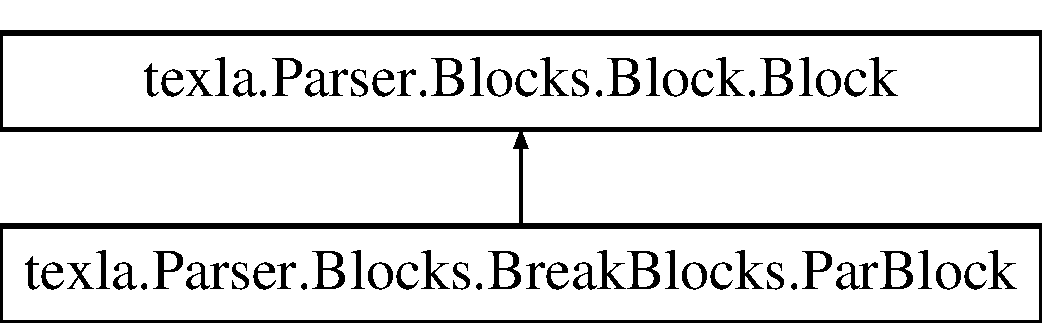
\includegraphics[height=2.000000cm]{classtexla_1_1Parser_1_1Blocks_1_1BreakBlocks_1_1ParBlock}
\end{center}
\end{figure}
\subsection*{Public Member Functions}
\begin{DoxyCompactItemize}
\item 
\hypertarget{classtexla_1_1Parser_1_1Blocks_1_1BreakBlocks_1_1ParBlock_a23a2ed3e8b2828fe3a4399c18f430280}{}\label{classtexla_1_1Parser_1_1Blocks_1_1BreakBlocks_1_1ParBlock_a23a2ed3e8b2828fe3a4399c18f430280} 
def {\bfseries \+\_\+\+\_\+init\+\_\+\+\_\+} (self, parent\+\_\+block)
\end{DoxyCompactItemize}
\subsection*{Static Public Member Functions}
\begin{DoxyCompactItemize}
\item 
\hypertarget{classtexla_1_1Parser_1_1Blocks_1_1BreakBlocks_1_1ParBlock_a9381ac510036f85bfe5161db586af907}{}\label{classtexla_1_1Parser_1_1Blocks_1_1BreakBlocks_1_1ParBlock_a9381ac510036f85bfe5161db586af907} 
def {\bfseries parse} (parser, tex, parent\+\_\+block, params)
\end{DoxyCompactItemize}
\subsection*{Additional Inherited Members}


\subsection{Detailed Description}
\begin{DoxyVerb}This block only represents a \n\n in the tex\end{DoxyVerb}
 

The documentation for this class was generated from the following file\+:\begin{DoxyCompactItemize}
\item 
texla/\+Parser/\+Blocks/Break\+Blocks.\+py\end{DoxyCompactItemize}

\hypertarget{classtexla_1_1Parser_1_1Parser_1_1Parser}{}\section{texla.\+Parser.\+Parser.\+Parser Class Reference}
\label{classtexla_1_1Parser_1_1Parser_1_1Parser}\index{texla.\+Parser.\+Parser.\+Parser@{texla.\+Parser.\+Parser.\+Parser}}
\subsection*{Public Member Functions}
\begin{DoxyCompactItemize}
\item 
\hypertarget{classtexla_1_1Parser_1_1Parser_1_1Parser_aa60009122c54ff992915770470fefbe8}{}\label{classtexla_1_1Parser_1_1Parser_1_1Parser_aa60009122c54ff992915770470fefbe8} 
def {\bfseries \+\_\+\+\_\+init\+\_\+\+\_\+} (self, configs)
\item 
def \hyperlink{classtexla_1_1Parser_1_1Parser_1_1Parser_afb55891b1d2f77a2e3aeeeb7f7e63550}{parse} (self, tex)
\item 
def \hyperlink{classtexla_1_1Parser_1_1Parser_1_1Parser_a7f65437398ebf3111c428747fdac9489}{parse\+\_\+sections} (self, tex, level, parent\+\_\+block, options)
\item 
def \hyperlink{classtexla_1_1Parser_1_1Parser_1_1Parser_a4c403acf107ba47795b70391db7e4bd4}{parse\+\_\+instructions} (self, tex, parent\+\_\+block, options)
\item 
def \hyperlink{classtexla_1_1Parser_1_1Parser_1_1Parser_ae5a596144e7be79cbca63d05dce99f06}{parse\+\_\+enviroment} (self, tex, parent\+\_\+block, options)
\item 
def \hyperlink{classtexla_1_1Parser_1_1Parser_1_1Parser_aee9adc1fcfa4c8194e37552124f67848}{parse\+\_\+math} (self, tex, parent\+\_\+block, options)
\item 
def \hyperlink{classtexla_1_1Parser_1_1Parser_1_1Parser_ac878c2e3e4690f9975ccf541b11796b5}{parse\+\_\+command} (self, tex, parent\+\_\+block, options)
\item 
def \hyperlink{classtexla_1_1Parser_1_1Parser_1_1Parser_a2ce55a1ea4d024ff77ce3a3718b76bbd}{parse\+\_\+commands\+\_\+group} (self, tex, parent\+\_\+block, options)
\item 
def \hyperlink{classtexla_1_1Parser_1_1Parser_1_1Parser_a66a08e68dd0a879d09ed5be4b41eb4b9}{parse\+\_\+letter\+\_\+command} (self, tex, parent\+\_\+block, options)
\item 
def \hyperlink{classtexla_1_1Parser_1_1Parser_1_1Parser_af4a46e7760e444cd77edf24053eb2cad}{parse\+\_\+special\+\_\+character} (self, tex, parent\+\_\+block, options)
\item 
def \hyperlink{classtexla_1_1Parser_1_1Parser_1_1Parser_af5273483c94bc329e6ec18d67967ce4a}{parse\+\_\+plain\+\_\+text} (self, tex, parent\+\_\+block)
\item 
def \hyperlink{classtexla_1_1Parser_1_1Parser_1_1Parser_a7fa931c1a8b0b570977fb5c311ea9ec0}{call\+\_\+parser\+\_\+hook} (self, hook, type, tex, parent\+\_\+block, params=\{\})
\end{DoxyCompactItemize}
\subsection*{Public Attributes}
\begin{DoxyCompactItemize}
\item 
\hypertarget{classtexla_1_1Parser_1_1Parser_1_1Parser_ae261ebc4805082d9e913ac94fddbbf2c}{}\label{classtexla_1_1Parser_1_1Parser_1_1Parser_ae261ebc4805082d9e913ac94fddbbf2c} 
{\bfseries configs}
\item 
\hypertarget{classtexla_1_1Parser_1_1Parser_1_1Parser_a7b3170987364bf71a42581ff7d768002}{}\label{classtexla_1_1Parser_1_1Parser_1_1Parser_a7b3170987364bf71a42581ff7d768002} 
{\bfseries doc\+\_\+data}
\item 
\hypertarget{classtexla_1_1Parser_1_1Parser_1_1Parser_a64d8a35b7496d8dfd1046cd74ea91500}{}\label{classtexla_1_1Parser_1_1Parser_1_1Parser_a64d8a35b7496d8dfd1046cd74ea91500} 
{\bfseries root\+\_\+block}
\item 
\hypertarget{classtexla_1_1Parser_1_1Parser_1_1Parser_aa71568a987d222cca941991fcb7d0f92}{}\label{classtexla_1_1Parser_1_1Parser_1_1Parser_aa71568a987d222cca941991fcb7d0f92} 
{\bfseries tree\+\_\+explorer}
\end{DoxyCompactItemize}


\subsection{Member Function Documentation}
\hypertarget{classtexla_1_1Parser_1_1Parser_1_1Parser_a7fa931c1a8b0b570977fb5c311ea9ec0}{}\label{classtexla_1_1Parser_1_1Parser_1_1Parser_a7fa931c1a8b0b570977fb5c311ea9ec0} 
\index{texla\+::\+Parser\+::\+Parser\+::\+Parser@{texla\+::\+Parser\+::\+Parser\+::\+Parser}!call\+\_\+parser\+\_\+hook@{call\+\_\+parser\+\_\+hook}}
\index{call\+\_\+parser\+\_\+hook@{call\+\_\+parser\+\_\+hook}!texla\+::\+Parser\+::\+Parser\+::\+Parser@{texla\+::\+Parser\+::\+Parser\+::\+Parser}}
\subsubsection{\texorpdfstring{call\+\_\+parser\+\_\+hook()}{call\_parser\_hook()}}
{\footnotesize\ttfamily def texla.\+Parser.\+Parser.\+Parser.\+call\+\_\+parser\+\_\+hook (\begin{DoxyParamCaption}\item[{}]{self,  }\item[{}]{hook,  }\item[{}]{type,  }\item[{}]{tex,  }\item[{}]{parent\+\_\+block,  }\item[{}]{params = {\ttfamily \{\}} }\end{DoxyParamCaption})}

\begin{DoxyVerb}This function checks if the required parser_hook
is avaiable, if not it calls th default hook.
The function ask for type of call (env or cmd)
to be able of asking the right default hooks,
in case the hook in not avaiable.
Params is a dictionary of options for the parser. It
usually contains che env or cmd parsed and if it's
starred.
It returns directly the output of parser_hook.
\end{DoxyVerb}
 \hypertarget{classtexla_1_1Parser_1_1Parser_1_1Parser_afb55891b1d2f77a2e3aeeeb7f7e63550}{}\label{classtexla_1_1Parser_1_1Parser_1_1Parser_afb55891b1d2f77a2e3aeeeb7f7e63550} 
\index{texla\+::\+Parser\+::\+Parser\+::\+Parser@{texla\+::\+Parser\+::\+Parser\+::\+Parser}!parse@{parse}}
\index{parse@{parse}!texla\+::\+Parser\+::\+Parser\+::\+Parser@{texla\+::\+Parser\+::\+Parser\+::\+Parser}}
\subsubsection{\texorpdfstring{parse()}{parse()}}
{\footnotesize\ttfamily def texla.\+Parser.\+Parser.\+Parser.\+parse (\begin{DoxyParamCaption}\item[{}]{self,  }\item[{}]{tex }\end{DoxyParamCaption})}

\begin{DoxyVerb}Entry point for parsing.
The DocumentBlock is created and all the
parse chain is started from parse_sections.
The function returns the root_block,
which contains all the parsed tree blocks.\end{DoxyVerb}
 \hypertarget{classtexla_1_1Parser_1_1Parser_1_1Parser_ac878c2e3e4690f9975ccf541b11796b5}{}\label{classtexla_1_1Parser_1_1Parser_1_1Parser_ac878c2e3e4690f9975ccf541b11796b5} 
\index{texla\+::\+Parser\+::\+Parser\+::\+Parser@{texla\+::\+Parser\+::\+Parser\+::\+Parser}!parse\+\_\+command@{parse\+\_\+command}}
\index{parse\+\_\+command@{parse\+\_\+command}!texla\+::\+Parser\+::\+Parser\+::\+Parser@{texla\+::\+Parser\+::\+Parser\+::\+Parser}}
\subsubsection{\texorpdfstring{parse\+\_\+command()}{parse\_command()}}
{\footnotesize\ttfamily def texla.\+Parser.\+Parser.\+Parser.\+parse\+\_\+command (\begin{DoxyParamCaption}\item[{}]{self,  }\item[{}]{tex,  }\item[{}]{parent\+\_\+block,  }\item[{}]{options }\end{DoxyParamCaption})}

\begin{DoxyVerb}This function handles the parsing of normal
commands. It catches the command's name and if it's
starred. Removed the \cmd part, the tex is passed
to the right parser_hook that manages the real
parsing of commands options. The parser_hook decides
also if the content of the command must be parsed
recursively.
It returns the block and the left tex that must
be parsed by another cycle of parse_instructions()
\end{DoxyVerb}
 \hypertarget{classtexla_1_1Parser_1_1Parser_1_1Parser_a2ce55a1ea4d024ff77ce3a3718b76bbd}{}\label{classtexla_1_1Parser_1_1Parser_1_1Parser_a2ce55a1ea4d024ff77ce3a3718b76bbd} 
\index{texla\+::\+Parser\+::\+Parser\+::\+Parser@{texla\+::\+Parser\+::\+Parser\+::\+Parser}!parse\+\_\+commands\+\_\+group@{parse\+\_\+commands\+\_\+group}}
\index{parse\+\_\+commands\+\_\+group@{parse\+\_\+commands\+\_\+group}!texla\+::\+Parser\+::\+Parser\+::\+Parser@{texla\+::\+Parser\+::\+Parser\+::\+Parser}}
\subsubsection{\texorpdfstring{parse\+\_\+commands\+\_\+group()}{parse\_commands\_group()}}
{\footnotesize\ttfamily def texla.\+Parser.\+Parser.\+Parser.\+parse\+\_\+commands\+\_\+group (\begin{DoxyParamCaption}\item[{}]{self,  }\item[{}]{tex,  }\item[{}]{parent\+\_\+block,  }\item[{}]{options }\end{DoxyParamCaption})}

\begin{DoxyVerb}This function handles the group of commands created
with the syntax {...}. It's used for the formatting
commands.
\end{DoxyVerb}
 \hypertarget{classtexla_1_1Parser_1_1Parser_1_1Parser_ae5a596144e7be79cbca63d05dce99f06}{}\label{classtexla_1_1Parser_1_1Parser_1_1Parser_ae5a596144e7be79cbca63d05dce99f06} 
\index{texla\+::\+Parser\+::\+Parser\+::\+Parser@{texla\+::\+Parser\+::\+Parser\+::\+Parser}!parse\+\_\+enviroment@{parse\+\_\+enviroment}}
\index{parse\+\_\+enviroment@{parse\+\_\+enviroment}!texla\+::\+Parser\+::\+Parser\+::\+Parser@{texla\+::\+Parser\+::\+Parser\+::\+Parser}}
\subsubsection{\texorpdfstring{parse\+\_\+enviroment()}{parse\_enviroment()}}
{\footnotesize\ttfamily def texla.\+Parser.\+Parser.\+Parser.\+parse\+\_\+enviroment (\begin{DoxyParamCaption}\item[{}]{self,  }\item[{}]{tex,  }\item[{}]{parent\+\_\+block,  }\item[{}]{options }\end{DoxyParamCaption})}

\begin{DoxyVerb}This function handles the parsing of environments.
It parses the name of the environment and if it's starred.
Then EnvironmentParser.get_environment() is used to extract
the complete environment, handling nested envs.
The content is sent to parser_hook for the specific parsing.
The parser_hook decides also if the content of the env
must be parsed recursively.
A new block is created and returned with the tex
remained to parse.
\end{DoxyVerb}
 \hypertarget{classtexla_1_1Parser_1_1Parser_1_1Parser_a4c403acf107ba47795b70391db7e4bd4}{}\label{classtexla_1_1Parser_1_1Parser_1_1Parser_a4c403acf107ba47795b70391db7e4bd4} 
\index{texla\+::\+Parser\+::\+Parser\+::\+Parser@{texla\+::\+Parser\+::\+Parser\+::\+Parser}!parse\+\_\+instructions@{parse\+\_\+instructions}}
\index{parse\+\_\+instructions@{parse\+\_\+instructions}!texla\+::\+Parser\+::\+Parser\+::\+Parser@{texla\+::\+Parser\+::\+Parser\+::\+Parser}}
\subsubsection{\texorpdfstring{parse\+\_\+instructions()}{parse\_instructions()}}
{\footnotesize\ttfamily def texla.\+Parser.\+Parser.\+Parser.\+parse\+\_\+instructions (\begin{DoxyParamCaption}\item[{}]{self,  }\item[{}]{tex,  }\item[{}]{parent\+\_\+block,  }\item[{}]{options }\end{DoxyParamCaption})}

\begin{DoxyVerb}This function is the MAIN ENTRY POINT for parsing.
It scan the tex from left to right. It searches for
\\ or $. When an instruction is found (a pattern starting
with \\ or $), the right parser function is called.
These functions take care to parse the command,
create the block calling parser_hooks, and to return
the block and the tex left to parse. Then the remaining
tex starts a new cycle in parse_instructions() recursively.
It returnes a list of parsed blocks.

The categories of instrucions parsed are:
-math: starts with $, $$ or \[ \(
-environments: (start with \begin)
-letters commands: they are special commands
    listed in letters_commands. They are
    parsed separately
-normal commands: like \cmd{text}
\end{DoxyVerb}
 \hypertarget{classtexla_1_1Parser_1_1Parser_1_1Parser_a66a08e68dd0a879d09ed5be4b41eb4b9}{}\label{classtexla_1_1Parser_1_1Parser_1_1Parser_a66a08e68dd0a879d09ed5be4b41eb4b9} 
\index{texla\+::\+Parser\+::\+Parser\+::\+Parser@{texla\+::\+Parser\+::\+Parser\+::\+Parser}!parse\+\_\+letter\+\_\+command@{parse\+\_\+letter\+\_\+command}}
\index{parse\+\_\+letter\+\_\+command@{parse\+\_\+letter\+\_\+command}!texla\+::\+Parser\+::\+Parser\+::\+Parser@{texla\+::\+Parser\+::\+Parser\+::\+Parser}}
\subsubsection{\texorpdfstring{parse\+\_\+letter\+\_\+command()}{parse\_letter\_command()}}
{\footnotesize\ttfamily def texla.\+Parser.\+Parser.\+Parser.\+parse\+\_\+letter\+\_\+command (\begin{DoxyParamCaption}\item[{}]{self,  }\item[{}]{tex,  }\item[{}]{parent\+\_\+block,  }\item[{}]{options }\end{DoxyParamCaption})}

\begin{DoxyVerb}'
This function handles special commands for accented
or modified letters.
They are special commands because they don't need a {}
and they act directly on the next letter.
Examples:
\'a: accented letter
\`a: grave accent
\~a \=a \^a other changes on the letter

The function parse that commands and call
parser_hook as the normal parse_command() function.
Althought, the letter influenced by the command is
inserted in a {} so that special command could
be treated like normal commands with hooks.
It returns the block and the left tex to parse.
\end{DoxyVerb}
 \hypertarget{classtexla_1_1Parser_1_1Parser_1_1Parser_aee9adc1fcfa4c8194e37552124f67848}{}\label{classtexla_1_1Parser_1_1Parser_1_1Parser_aee9adc1fcfa4c8194e37552124f67848} 
\index{texla\+::\+Parser\+::\+Parser\+::\+Parser@{texla\+::\+Parser\+::\+Parser\+::\+Parser}!parse\+\_\+math@{parse\+\_\+math}}
\index{parse\+\_\+math@{parse\+\_\+math}!texla\+::\+Parser\+::\+Parser\+::\+Parser@{texla\+::\+Parser\+::\+Parser\+::\+Parser}}
\subsubsection{\texorpdfstring{parse\+\_\+math()}{parse\_math()}}
{\footnotesize\ttfamily def texla.\+Parser.\+Parser.\+Parser.\+parse\+\_\+math (\begin{DoxyParamCaption}\item[{}]{self,  }\item[{}]{tex,  }\item[{}]{parent\+\_\+block,  }\item[{}]{options }\end{DoxyParamCaption})}

\begin{DoxyVerb}This function handles the parsing of math commands:
$..$, $$..$$, \[..\], \(..\). The matched math
is inserted in "display_math" or "inline_math" block.
The function returnes the block and left_tex.
\end{DoxyVerb}
 \hypertarget{classtexla_1_1Parser_1_1Parser_1_1Parser_af5273483c94bc329e6ec18d67967ce4a}{}\label{classtexla_1_1Parser_1_1Parser_1_1Parser_af5273483c94bc329e6ec18d67967ce4a} 
\index{texla\+::\+Parser\+::\+Parser\+::\+Parser@{texla\+::\+Parser\+::\+Parser\+::\+Parser}!parse\+\_\+plain\+\_\+text@{parse\+\_\+plain\+\_\+text}}
\index{parse\+\_\+plain\+\_\+text@{parse\+\_\+plain\+\_\+text}!texla\+::\+Parser\+::\+Parser\+::\+Parser@{texla\+::\+Parser\+::\+Parser\+::\+Parser}}
\subsubsection{\texorpdfstring{parse\+\_\+plain\+\_\+text()}{parse\_plain\_text()}}
{\footnotesize\ttfamily def texla.\+Parser.\+Parser.\+Parser.\+parse\+\_\+plain\+\_\+text (\begin{DoxyParamCaption}\item[{}]{self,  }\item[{}]{tex,  }\item[{}]{parent\+\_\+block }\end{DoxyParamCaption})}

\begin{DoxyVerb}This function create the block for plain text.
It doesn't return any left tex.
\end{DoxyVerb}
 \hypertarget{classtexla_1_1Parser_1_1Parser_1_1Parser_a7f65437398ebf3111c428747fdac9489}{}\label{classtexla_1_1Parser_1_1Parser_1_1Parser_a7f65437398ebf3111c428747fdac9489} 
\index{texla\+::\+Parser\+::\+Parser\+::\+Parser@{texla\+::\+Parser\+::\+Parser\+::\+Parser}!parse\+\_\+sections@{parse\+\_\+sections}}
\index{parse\+\_\+sections@{parse\+\_\+sections}!texla\+::\+Parser\+::\+Parser\+::\+Parser@{texla\+::\+Parser\+::\+Parser\+::\+Parser}}
\subsubsection{\texorpdfstring{parse\+\_\+sections()}{parse\_sections()}}
{\footnotesize\ttfamily def texla.\+Parser.\+Parser.\+Parser.\+parse\+\_\+sections (\begin{DoxyParamCaption}\item[{}]{self,  }\item[{}]{tex,  }\item[{}]{level,  }\item[{}]{parent\+\_\+block,  }\item[{}]{options }\end{DoxyParamCaption})}

\begin{DoxyVerb}This parser function search for sections splitting inside tex.
The level of sections searched is indicated by sec_level option.
The function calls the parser_hooks of every section block.
When all sections levels are searched the control
pass to parse_instructions().
It returns a list of blocks parsed as tuples.
\end{DoxyVerb}
 \hypertarget{classtexla_1_1Parser_1_1Parser_1_1Parser_af4a46e7760e444cd77edf24053eb2cad}{}\label{classtexla_1_1Parser_1_1Parser_1_1Parser_af4a46e7760e444cd77edf24053eb2cad} 
\index{texla\+::\+Parser\+::\+Parser\+::\+Parser@{texla\+::\+Parser\+::\+Parser\+::\+Parser}!parse\+\_\+special\+\_\+character@{parse\+\_\+special\+\_\+character}}
\index{parse\+\_\+special\+\_\+character@{parse\+\_\+special\+\_\+character}!texla\+::\+Parser\+::\+Parser\+::\+Parser@{texla\+::\+Parser\+::\+Parser\+::\+Parser}}
\subsubsection{\texorpdfstring{parse\+\_\+special\+\_\+character()}{parse\_special\_character()}}
{\footnotesize\ttfamily def texla.\+Parser.\+Parser.\+Parser.\+parse\+\_\+special\+\_\+character (\begin{DoxyParamCaption}\item[{}]{self,  }\item[{}]{tex,  }\item[{}]{parent\+\_\+block,  }\item[{}]{options }\end{DoxyParamCaption})}

\begin{DoxyVerb}This function parse special commands like \% or \&.
The mechanism is the same ad special_commands, but options
are not searched.
\end{DoxyVerb}
 

The documentation for this class was generated from the following file\+:\begin{DoxyCompactItemize}
\item 
texla/\+Parser/Parser.\+py\end{DoxyCompactItemize}

\hypertarget{classtexla_1_1Parser_1_1Blocks_1_1TheoremBlocks_1_1ProofBlock}{}\section{texla.\+Parser.\+Blocks.\+Theorem\+Blocks.\+Proof\+Block Class Reference}
\label{classtexla_1_1Parser_1_1Blocks_1_1TheoremBlocks_1_1ProofBlock}\index{texla.\+Parser.\+Blocks.\+Theorem\+Blocks.\+Proof\+Block@{texla.\+Parser.\+Blocks.\+Theorem\+Blocks.\+Proof\+Block}}
Inheritance diagram for texla.\+Parser.\+Blocks.\+Theorem\+Blocks.\+Proof\+Block\+:\begin{figure}[H]
\begin{center}
\leavevmode
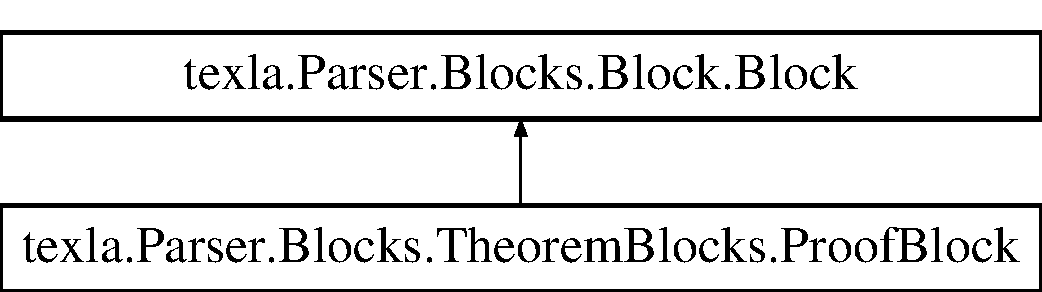
\includegraphics[height=2.000000cm]{classtexla_1_1Parser_1_1Blocks_1_1TheoremBlocks_1_1ProofBlock}
\end{center}
\end{figure}
\subsection*{Public Member Functions}
\begin{DoxyCompactItemize}
\item 
\hypertarget{classtexla_1_1Parser_1_1Blocks_1_1TheoremBlocks_1_1ProofBlock_a5f38f05ef77faad7ef9c306af35807e8}{}\label{classtexla_1_1Parser_1_1Blocks_1_1TheoremBlocks_1_1ProofBlock_a5f38f05ef77faad7ef9c306af35807e8} 
def {\bfseries \+\_\+\+\_\+init\+\_\+\+\_\+} (self, title, content, parent\+\_\+block)
\end{DoxyCompactItemize}
\subsection*{Static Public Member Functions}
\begin{DoxyCompactItemize}
\item 
\hypertarget{classtexla_1_1Parser_1_1Blocks_1_1TheoremBlocks_1_1ProofBlock_a949c75a021a513290ee5b5039ecd3deb}{}\label{classtexla_1_1Parser_1_1Blocks_1_1TheoremBlocks_1_1ProofBlock_a949c75a021a513290ee5b5039ecd3deb} 
def {\bfseries parse} (parser, tex, parent\+\_\+block, params)
\end{DoxyCompactItemize}
\subsection*{Public Attributes}
\begin{DoxyCompactItemize}
\item 
\hypertarget{classtexla_1_1Parser_1_1Blocks_1_1TheoremBlocks_1_1ProofBlock_a1c553c16331caf7ad258c8e88ccb3b58}{}\label{classtexla_1_1Parser_1_1Blocks_1_1TheoremBlocks_1_1ProofBlock_a1c553c16331caf7ad258c8e88ccb3b58} 
{\bfseries title}
\end{DoxyCompactItemize}


\subsection{Detailed Description}
\begin{DoxyVerb}Block that represents a proof.\end{DoxyVerb}
 

The documentation for this class was generated from the following file\+:\begin{DoxyCompactItemize}
\item 
texla/\+Parser/\+Blocks/Theorem\+Blocks.\+py\end{DoxyCompactItemize}

\hypertarget{classtexla_1_1Parser_1_1Blocks_1_1NoteBlocks_1_1QuotationBlock}{}\section{texla.\+Parser.\+Blocks.\+Note\+Blocks.\+Quotation\+Block Class Reference}
\label{classtexla_1_1Parser_1_1Blocks_1_1NoteBlocks_1_1QuotationBlock}\index{texla.\+Parser.\+Blocks.\+Note\+Blocks.\+Quotation\+Block@{texla.\+Parser.\+Blocks.\+Note\+Blocks.\+Quotation\+Block}}
Inheritance diagram for texla.\+Parser.\+Blocks.\+Note\+Blocks.\+Quotation\+Block\+:\begin{figure}[H]
\begin{center}
\leavevmode
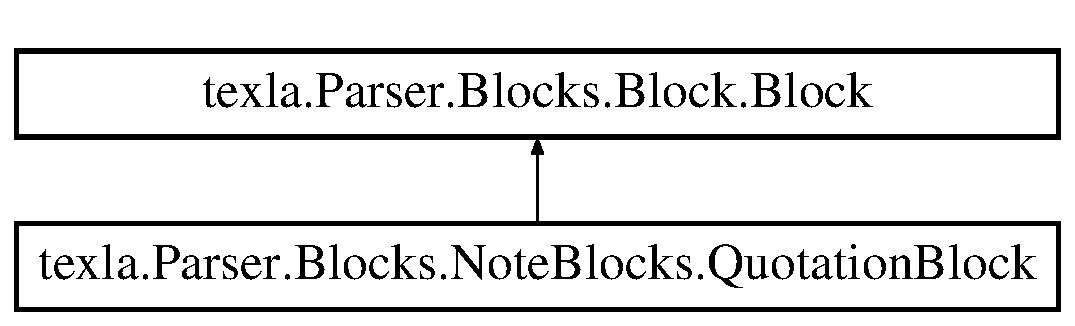
\includegraphics[height=2.000000cm]{classtexla_1_1Parser_1_1Blocks_1_1NoteBlocks_1_1QuotationBlock}
\end{center}
\end{figure}
\subsection*{Public Member Functions}
\begin{DoxyCompactItemize}
\item 
\hypertarget{classtexla_1_1Parser_1_1Blocks_1_1NoteBlocks_1_1QuotationBlock_ad369a479e46a782bdc2b096fe15f3d1d}{}\label{classtexla_1_1Parser_1_1Blocks_1_1NoteBlocks_1_1QuotationBlock_ad369a479e46a782bdc2b096fe15f3d1d} 
def {\bfseries \+\_\+\+\_\+init\+\_\+\+\_\+} (self, tex, quote\+\_\+type, parent\+\_\+block)
\end{DoxyCompactItemize}
\subsection*{Static Public Member Functions}
\begin{DoxyCompactItemize}
\item 
\hypertarget{classtexla_1_1Parser_1_1Blocks_1_1NoteBlocks_1_1QuotationBlock_a755d927388a76e7f5eaf1792c5f733c0}{}\label{classtexla_1_1Parser_1_1Blocks_1_1NoteBlocks_1_1QuotationBlock_a755d927388a76e7f5eaf1792c5f733c0} 
def {\bfseries parse} (parser, tex, parent\+\_\+block, params)
\end{DoxyCompactItemize}
\subsection*{Public Attributes}
\begin{DoxyCompactItemize}
\item 
\hypertarget{classtexla_1_1Parser_1_1Blocks_1_1NoteBlocks_1_1QuotationBlock_a98c2904651896fef591b5feda9cf2646}{}\label{classtexla_1_1Parser_1_1Blocks_1_1NoteBlocks_1_1QuotationBlock_a98c2904651896fef591b5feda9cf2646} 
{\bfseries quote\+\_\+type}
\end{DoxyCompactItemize}


The documentation for this class was generated from the following file\+:\begin{DoxyCompactItemize}
\item 
texla/\+Parser/\+Blocks/Note\+Blocks.\+py\end{DoxyCompactItemize}

\hypertarget{classtexla_1_1Parser_1_1Blocks_1_1ReferenceBlocks_1_1RefBlock}{}\section{texla.\+Parser.\+Blocks.\+Reference\+Blocks.\+Ref\+Block Class Reference}
\label{classtexla_1_1Parser_1_1Blocks_1_1ReferenceBlocks_1_1RefBlock}\index{texla.\+Parser.\+Blocks.\+Reference\+Blocks.\+Ref\+Block@{texla.\+Parser.\+Blocks.\+Reference\+Blocks.\+Ref\+Block}}
Inheritance diagram for texla.\+Parser.\+Blocks.\+Reference\+Blocks.\+Ref\+Block\+:\begin{figure}[H]
\begin{center}
\leavevmode
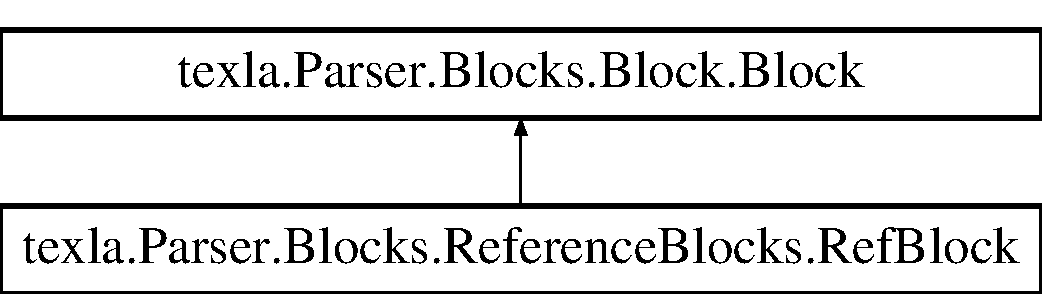
\includegraphics[height=2.000000cm]{classtexla_1_1Parser_1_1Blocks_1_1ReferenceBlocks_1_1RefBlock}
\end{center}
\end{figure}
\subsection*{Public Member Functions}
\begin{DoxyCompactItemize}
\item 
\hypertarget{classtexla_1_1Parser_1_1Blocks_1_1ReferenceBlocks_1_1RefBlock_a9534ccf3ca3cf585e4a8f9f692d0a347}{}\label{classtexla_1_1Parser_1_1Blocks_1_1ReferenceBlocks_1_1RefBlock_a9534ccf3ca3cf585e4a8f9f692d0a347} 
def {\bfseries \+\_\+\+\_\+init\+\_\+\+\_\+} (self, ref, ref\+\_\+type, parent\+\_\+block)
\item 
\hypertarget{classtexla_1_1Parser_1_1Blocks_1_1ReferenceBlocks_1_1RefBlock_a6eb2d28fe8dd4fe4aeedfca0d9bc0190}{}\label{classtexla_1_1Parser_1_1Blocks_1_1ReferenceBlocks_1_1RefBlock_a6eb2d28fe8dd4fe4aeedfca0d9bc0190} 
def {\bfseries \+\_\+\+\_\+str\+\_\+\+\_\+} (self)
\end{DoxyCompactItemize}
\subsection*{Static Public Member Functions}
\begin{DoxyCompactItemize}
\item 
\hypertarget{classtexla_1_1Parser_1_1Blocks_1_1ReferenceBlocks_1_1RefBlock_a5070acc406d4b3b8da49845e910c09e9}{}\label{classtexla_1_1Parser_1_1Blocks_1_1ReferenceBlocks_1_1RefBlock_a5070acc406d4b3b8da49845e910c09e9} 
def {\bfseries parse\+\_\+ref} (parser, tex, parent\+\_\+block, params)
\end{DoxyCompactItemize}
\subsection*{Public Attributes}
\begin{DoxyCompactItemize}
\item 
\hypertarget{classtexla_1_1Parser_1_1Blocks_1_1ReferenceBlocks_1_1RefBlock_a31d461676ff0abaf7c81b9f997a169b5}{}\label{classtexla_1_1Parser_1_1Blocks_1_1ReferenceBlocks_1_1RefBlock_a31d461676ff0abaf7c81b9f997a169b5} 
{\bfseries ref}
\item 
\hypertarget{classtexla_1_1Parser_1_1Blocks_1_1ReferenceBlocks_1_1RefBlock_a60075d90c8af5e8dda3756af925f1aa4}{}\label{classtexla_1_1Parser_1_1Blocks_1_1ReferenceBlocks_1_1RefBlock_a60075d90c8af5e8dda3756af925f1aa4} 
{\bfseries ref\+\_\+type}
\end{DoxyCompactItemize}


\subsection{Detailed Description}
\begin{DoxyVerb}Block thar represents reference\end{DoxyVerb}
 

The documentation for this class was generated from the following file\+:\begin{DoxyCompactItemize}
\item 
texla/\+Parser/\+Blocks/Reference\+Blocks.\+py\end{DoxyCompactItemize}

\hypertarget{classtexla_1_1Renderers_1_1Renderer_1_1Renderer}{}\section{texla.\+Renderers.\+Renderer.\+Renderer Class Reference}
\label{classtexla_1_1Renderers_1_1Renderer_1_1Renderer}\index{texla.\+Renderers.\+Renderer.\+Renderer@{texla.\+Renderers.\+Renderer.\+Renderer}}
Inheritance diagram for texla.\+Renderers.\+Renderer.\+Renderer\+:\begin{figure}[H]
\begin{center}
\leavevmode
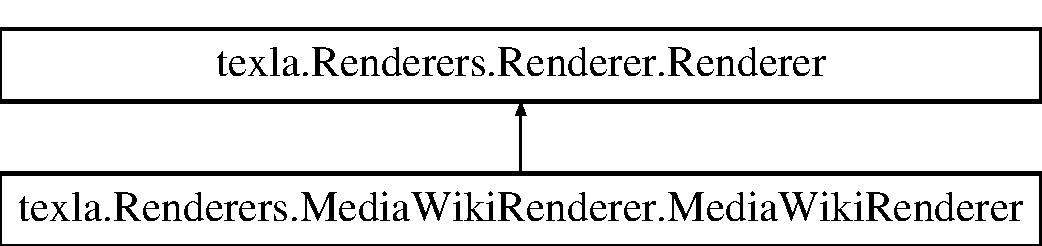
\includegraphics[height=2.000000cm]{classtexla_1_1Renderers_1_1Renderer_1_1Renderer}
\end{center}
\end{figure}
\subsection*{Public Member Functions}
\begin{DoxyCompactItemize}
\item 
\hypertarget{classtexla_1_1Renderers_1_1Renderer_1_1Renderer_ad7b2d2ad9bd47d4ca6e01efdd9f794bd}{}\label{classtexla_1_1Renderers_1_1Renderer_1_1Renderer_ad7b2d2ad9bd47d4ca6e01efdd9f794bd} 
def {\bfseries \+\_\+\+\_\+init\+\_\+\+\_\+} (self)
\item 
\hypertarget{classtexla_1_1Renderers_1_1Renderer_1_1Renderer_aa65e78017d10f6ccaacf0dffcd009668}{}\label{classtexla_1_1Renderers_1_1Renderer_1_1Renderer_aa65e78017d10f6ccaacf0dffcd009668} 
def {\bfseries register\+\_\+plugins} (self, plugins)
\item 
def \hyperlink{classtexla_1_1Renderers_1_1Renderer_1_1Renderer_ab2a50912d83684b9cd57fc4feccedad6}{register\+\_\+render\+\_\+plugin\+\_\+hooks} (self, hooks)
\item 
def \hyperlink{classtexla_1_1Renderers_1_1Renderer_1_1Renderer_aa5ac1cc3c4e118189bd4497ed03564dd}{register\+\_\+lifecyle\+\_\+plugin\+\_\+hooks} (self, hooks)
\item 
\hypertarget{classtexla_1_1Renderers_1_1Renderer_1_1Renderer_aaea86a5a1ed0006da6fde82f716bfebe}{}\label{classtexla_1_1Renderers_1_1Renderer_1_1Renderer_aaea86a5a1ed0006da6fde82f716bfebe} 
def {\bfseries register\+\_\+pre\+\_\+renderer\+\_\+hook} (self, block, hook)
\item 
\hypertarget{classtexla_1_1Renderers_1_1Renderer_1_1Renderer_a4cedb88a4c46f5a01e2f16b7d432e485}{}\label{classtexla_1_1Renderers_1_1Renderer_1_1Renderer_a4cedb88a4c46f5a01e2f16b7d432e485} 
def {\bfseries register\+\_\+post\+\_\+renderer\+\_\+hook} (self, block, hook)
\item 
\hypertarget{classtexla_1_1Renderers_1_1Renderer_1_1Renderer_a347b7e0aa8e3040911e038fe916c329d}{}\label{classtexla_1_1Renderers_1_1Renderer_1_1Renderer_a347b7e0aa8e3040911e038fe916c329d} 
def {\bfseries register\+\_\+start\+\_\+hook} (self, hook)
\item 
\hypertarget{classtexla_1_1Renderers_1_1Renderer_1_1Renderer_a87c47afda693254e1e6ffaaea96e018b}{}\label{classtexla_1_1Renderers_1_1Renderer_1_1Renderer_a87c47afda693254e1e6ffaaea96e018b} 
def {\bfseries register\+\_\+end\+\_\+hook} (self, hook)
\item 
def \hyperlink{classtexla_1_1Renderers_1_1Renderer_1_1Renderer_a2f95c5cc5ea76c75cb5ee79df01f43f2}{start\+\_\+rendering} (self, root\+\_\+block)
\item 
\hypertarget{classtexla_1_1Renderers_1_1Renderer_1_1Renderer_a0c01fa2fc88f08a8ad3b4eb10a6cbf56}{}\label{classtexla_1_1Renderers_1_1Renderer_1_1Renderer_a0c01fa2fc88f08a8ad3b4eb10a6cbf56} 
def {\bfseries end\+\_\+rendering} (self)
\item 
def \hyperlink{classtexla_1_1Renderers_1_1Renderer_1_1Renderer_a3fda0b658f6e8b0215e2d9062d0f0893}{render\+\_\+children\+\_\+blocks} (self, block, collapse=True)
\item 
def \hyperlink{classtexla_1_1Renderers_1_1Renderer_1_1Renderer_ae58221b6a1aec6777d7e6d1bbc97e254}{render\+\_\+block} (self, bl)
\item 
def \hyperlink{classtexla_1_1Renderers_1_1Renderer_1_1Renderer_af8fccb30690606612e6c62851cd899fe}{render\+\_\+blocks} (self, bls, collapse=False)
\item 
\hypertarget{classtexla_1_1Renderers_1_1Renderer_1_1Renderer_a34cd4a95caeb1ffcc144fb71321ef671}{}\label{classtexla_1_1Renderers_1_1Renderer_1_1Renderer_a34cd4a95caeb1ffcc144fb71321ef671} 
def {\bfseries used\+\_\+tag} (self, tag)
\end{DoxyCompactItemize}
\subsection*{Public Attributes}
\begin{DoxyCompactItemize}
\item 
\hypertarget{classtexla_1_1Renderers_1_1Renderer_1_1Renderer_a67f648f712e75417371647e0c80cc4d6}{}\label{classtexla_1_1Renderers_1_1Renderer_1_1Renderer_a67f648f712e75417371647e0c80cc4d6} 
{\bfseries render\+\_\+hooks}
\item 
\hypertarget{classtexla_1_1Renderers_1_1Renderer_1_1Renderer_a9817075b382f7fa1e523d45ceda34120}{}\label{classtexla_1_1Renderers_1_1Renderer_1_1Renderer_a9817075b382f7fa1e523d45ceda34120} 
{\bfseries pre\+\_\+render\+\_\+hooks}
\item 
\hypertarget{classtexla_1_1Renderers_1_1Renderer_1_1Renderer_a41343907b1bd157e20b8a59e02952589}{}\label{classtexla_1_1Renderers_1_1Renderer_1_1Renderer_a41343907b1bd157e20b8a59e02952589} 
{\bfseries post\+\_\+render\+\_\+hooks}
\item 
\hypertarget{classtexla_1_1Renderers_1_1Renderer_1_1Renderer_afab236e28ee034c4fa98de6aa0cea432}{}\label{classtexla_1_1Renderers_1_1Renderer_1_1Renderer_afab236e28ee034c4fa98de6aa0cea432} 
{\bfseries start\+\_\+hooks}
\item 
\hypertarget{classtexla_1_1Renderers_1_1Renderer_1_1Renderer_add33cdbfb21b10e4cb7c4cc0591a590e}{}\label{classtexla_1_1Renderers_1_1Renderer_1_1Renderer_add33cdbfb21b10e4cb7c4cc0591a590e} 
{\bfseries end\+\_\+hooks}
\item 
\hypertarget{classtexla_1_1Renderers_1_1Renderer_1_1Renderer_aae7192fca7376ffb380c73155721ab68}{}\label{classtexla_1_1Renderers_1_1Renderer_1_1Renderer_aae7192fca7376ffb380c73155721ab68} 
{\bfseries loaded\+\_\+plugins}
\item 
\hypertarget{classtexla_1_1Renderers_1_1Renderer_1_1Renderer_a1cb0d0cfd8fcb07a31b0b3f69570e679}{}\label{classtexla_1_1Renderers_1_1Renderer_1_1Renderer_a1cb0d0cfd8fcb07a31b0b3f69570e679} 
{\bfseries used\+\_\+tags}
\item 
\hypertarget{classtexla_1_1Renderers_1_1Renderer_1_1Renderer_a045926ded0210c33c770f1d5aec3421d}{}\label{classtexla_1_1Renderers_1_1Renderer_1_1Renderer_a045926ded0210c33c770f1d5aec3421d} 
{\bfseries tree\+\_\+explorer}
\end{DoxyCompactItemize}


\subsection{Member Function Documentation}
\hypertarget{classtexla_1_1Renderers_1_1Renderer_1_1Renderer_aa5ac1cc3c4e118189bd4497ed03564dd}{}\label{classtexla_1_1Renderers_1_1Renderer_1_1Renderer_aa5ac1cc3c4e118189bd4497ed03564dd} 
\index{texla\+::\+Renderers\+::\+Renderer\+::\+Renderer@{texla\+::\+Renderers\+::\+Renderer\+::\+Renderer}!register\+\_\+lifecyle\+\_\+plugin\+\_\+hooks@{register\+\_\+lifecyle\+\_\+plugin\+\_\+hooks}}
\index{register\+\_\+lifecyle\+\_\+plugin\+\_\+hooks@{register\+\_\+lifecyle\+\_\+plugin\+\_\+hooks}!texla\+::\+Renderers\+::\+Renderer\+::\+Renderer@{texla\+::\+Renderers\+::\+Renderer\+::\+Renderer}}
\subsubsection{\texorpdfstring{register\+\_\+lifecyle\+\_\+plugin\+\_\+hooks()}{register\_lifecyle\_plugin\_hooks()}}
{\footnotesize\ttfamily def texla.\+Renderers.\+Renderer.\+Renderer.\+register\+\_\+lifecyle\+\_\+plugin\+\_\+hooks (\begin{DoxyParamCaption}\item[{}]{self,  }\item[{}]{hooks }\end{DoxyParamCaption})}

\begin{DoxyVerb}This function registers the hooks for the renderer lifecycle.
Plugins can register hooks for the start and end actions.
The start hook is called with the root_block of the chain.
The end hook is called without arguments. These hooks must be used
only to signal the actions to the plugins.\end{DoxyVerb}
 \hypertarget{classtexla_1_1Renderers_1_1Renderer_1_1Renderer_ab2a50912d83684b9cd57fc4feccedad6}{}\label{classtexla_1_1Renderers_1_1Renderer_1_1Renderer_ab2a50912d83684b9cd57fc4feccedad6} 
\index{texla\+::\+Renderers\+::\+Renderer\+::\+Renderer@{texla\+::\+Renderers\+::\+Renderer\+::\+Renderer}!register\+\_\+render\+\_\+plugin\+\_\+hooks@{register\+\_\+render\+\_\+plugin\+\_\+hooks}}
\index{register\+\_\+render\+\_\+plugin\+\_\+hooks@{register\+\_\+render\+\_\+plugin\+\_\+hooks}!texla\+::\+Renderers\+::\+Renderer\+::\+Renderer@{texla\+::\+Renderers\+::\+Renderer\+::\+Renderer}}
\subsubsection{\texorpdfstring{register\+\_\+render\+\_\+plugin\+\_\+hooks()}{register\_render\_plugin\_hooks()}}
{\footnotesize\ttfamily def texla.\+Renderers.\+Renderer.\+Renderer.\+register\+\_\+render\+\_\+plugin\+\_\+hooks (\begin{DoxyParamCaption}\item[{}]{self,  }\item[{}]{hooks }\end{DoxyParamCaption})}

\begin{DoxyVerb}This function registers the hooks for renderer plugins.
The plugins can define hooks for pre and post render actions.
The pre hook receives the block before the rendering and can
only return the block itself, modified.
The post hook receive the block and the text from the renderer:
it has to return the final text only.
The keyword ALL creates a hooks for all the blocks.
Note that it is always called after all the other hooks.\end{DoxyVerb}
 \hypertarget{classtexla_1_1Renderers_1_1Renderer_1_1Renderer_ae58221b6a1aec6777d7e6d1bbc97e254}{}\label{classtexla_1_1Renderers_1_1Renderer_1_1Renderer_ae58221b6a1aec6777d7e6d1bbc97e254} 
\index{texla\+::\+Renderers\+::\+Renderer\+::\+Renderer@{texla\+::\+Renderers\+::\+Renderer\+::\+Renderer}!render\+\_\+block@{render\+\_\+block}}
\index{render\+\_\+block@{render\+\_\+block}!texla\+::\+Renderers\+::\+Renderer\+::\+Renderer@{texla\+::\+Renderers\+::\+Renderer\+::\+Renderer}}
\subsubsection{\texorpdfstring{render\+\_\+block()}{render\_block()}}
{\footnotesize\ttfamily def texla.\+Renderers.\+Renderer.\+Renderer.\+render\+\_\+block (\begin{DoxyParamCaption}\item[{}]{self,  }\item[{}]{bl }\end{DoxyParamCaption})}

\begin{DoxyVerb}This function calls the right render_hook for
the block. If there isn't an hook it calld the default,
that is mandatory\end{DoxyVerb}
 \hypertarget{classtexla_1_1Renderers_1_1Renderer_1_1Renderer_af8fccb30690606612e6c62851cd899fe}{}\label{classtexla_1_1Renderers_1_1Renderer_1_1Renderer_af8fccb30690606612e6c62851cd899fe} 
\index{texla\+::\+Renderers\+::\+Renderer\+::\+Renderer@{texla\+::\+Renderers\+::\+Renderer\+::\+Renderer}!render\+\_\+blocks@{render\+\_\+blocks}}
\index{render\+\_\+blocks@{render\+\_\+blocks}!texla\+::\+Renderers\+::\+Renderer\+::\+Renderer@{texla\+::\+Renderers\+::\+Renderer\+::\+Renderer}}
\subsubsection{\texorpdfstring{render\+\_\+blocks()}{render\_blocks()}}
{\footnotesize\ttfamily def texla.\+Renderers.\+Renderer.\+Renderer.\+render\+\_\+blocks (\begin{DoxyParamCaption}\item[{}]{self,  }\item[{}]{bls,  }\item[{}]{collapse = {\ttfamily False} }\end{DoxyParamCaption})}

\begin{DoxyVerb}This function renderes a list of blocks.
It's the same as render_children_blocks but
with a generic list\end{DoxyVerb}
 \hypertarget{classtexla_1_1Renderers_1_1Renderer_1_1Renderer_a3fda0b658f6e8b0215e2d9062d0f0893}{}\label{classtexla_1_1Renderers_1_1Renderer_1_1Renderer_a3fda0b658f6e8b0215e2d9062d0f0893} 
\index{texla\+::\+Renderers\+::\+Renderer\+::\+Renderer@{texla\+::\+Renderers\+::\+Renderer\+::\+Renderer}!render\+\_\+children\+\_\+blocks@{render\+\_\+children\+\_\+blocks}}
\index{render\+\_\+children\+\_\+blocks@{render\+\_\+children\+\_\+blocks}!texla\+::\+Renderers\+::\+Renderer\+::\+Renderer@{texla\+::\+Renderers\+::\+Renderer\+::\+Renderer}}
\subsubsection{\texorpdfstring{render\+\_\+children\+\_\+blocks()}{render\_children\_blocks()}}
{\footnotesize\ttfamily def texla.\+Renderers.\+Renderer.\+Renderer.\+render\+\_\+children\+\_\+blocks (\begin{DoxyParamCaption}\item[{}]{self,  }\item[{}]{block,  }\item[{}]{collapse = {\ttfamily True} }\end{DoxyParamCaption})}

\begin{DoxyVerb}This is one of the most important funciont
of the rendering process.
This function takes all the children blocks of
a block and get they rendering output.
If collapsed=True it returns a unique string,
otherwise it returns a list of tuples with[(block_name, output)]
\end{DoxyVerb}
 \hypertarget{classtexla_1_1Renderers_1_1Renderer_1_1Renderer_a2f95c5cc5ea76c75cb5ee79df01f43f2}{}\label{classtexla_1_1Renderers_1_1Renderer_1_1Renderer_a2f95c5cc5ea76c75cb5ee79df01f43f2} 
\index{texla\+::\+Renderers\+::\+Renderer\+::\+Renderer@{texla\+::\+Renderers\+::\+Renderer\+::\+Renderer}!start\+\_\+rendering@{start\+\_\+rendering}}
\index{start\+\_\+rendering@{start\+\_\+rendering}!texla\+::\+Renderers\+::\+Renderer\+::\+Renderer@{texla\+::\+Renderers\+::\+Renderer\+::\+Renderer}}
\subsubsection{\texorpdfstring{start\+\_\+rendering()}{start\_rendering()}}
{\footnotesize\ttfamily def texla.\+Renderers.\+Renderer.\+Renderer.\+start\+\_\+rendering (\begin{DoxyParamCaption}\item[{}]{self,  }\item[{}]{root\+\_\+block }\end{DoxyParamCaption})}

\begin{DoxyVerb}This function create a TreeExplorer instance
and passes it to the plugin that has the variable
needs_tree_explorer=True. Then it starts the plugins\end{DoxyVerb}
 

The documentation for this class was generated from the following file\+:\begin{DoxyCompactItemize}
\item 
texla/\+Renderers/Renderer.\+py\end{DoxyCompactItemize}

\hypertarget{classtexla_1_1Parser_1_1Blocks_1_1SectionBlock_1_1SectionBlock}{}\section{texla.\+Parser.\+Blocks.\+Section\+Block.\+Section\+Block Class Reference}
\label{classtexla_1_1Parser_1_1Blocks_1_1SectionBlock_1_1SectionBlock}\index{texla.\+Parser.\+Blocks.\+Section\+Block.\+Section\+Block@{texla.\+Parser.\+Blocks.\+Section\+Block.\+Section\+Block}}
Inheritance diagram for texla.\+Parser.\+Blocks.\+Section\+Block.\+Section\+Block\+:\begin{figure}[H]
\begin{center}
\leavevmode
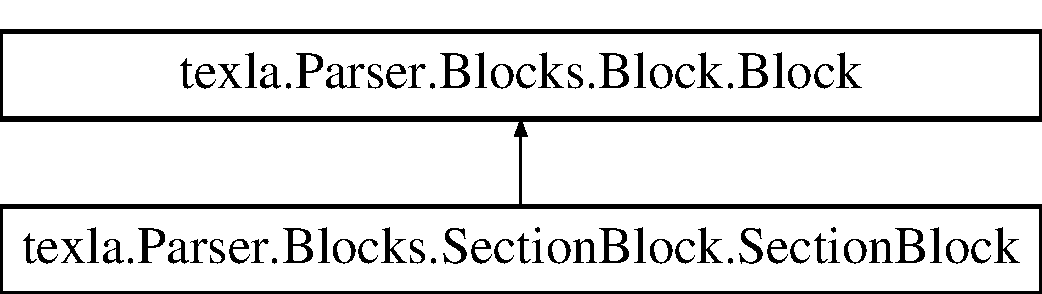
\includegraphics[height=2.000000cm]{classtexla_1_1Parser_1_1Blocks_1_1SectionBlock_1_1SectionBlock}
\end{center}
\end{figure}
\subsection*{Public Member Functions}
\begin{DoxyCompactItemize}
\item 
def \hyperlink{classtexla_1_1Parser_1_1Blocks_1_1SectionBlock_1_1SectionBlock_aaaffff6b091aa366f66ecfae3ec7b909}{\+\_\+\+\_\+init\+\_\+\+\_\+} (self, title, index\+\_\+title, star, level, parent\+\_\+block)
\item 
\hypertarget{classtexla_1_1Parser_1_1Blocks_1_1SectionBlock_1_1SectionBlock_aadad22f461c2e48cc651f6b78bd98b9b}{}\label{classtexla_1_1Parser_1_1Blocks_1_1SectionBlock_1_1SectionBlock_aadad22f461c2e48cc651f6b78bd98b9b} 
def {\bfseries \+\_\+\+\_\+str\+\_\+\+\_\+} (self)
\end{DoxyCompactItemize}
\subsection*{Static Public Member Functions}
\begin{DoxyCompactItemize}
\item 
\hypertarget{classtexla_1_1Parser_1_1Blocks_1_1SectionBlock_1_1SectionBlock_af23ad266eb0f4899bc88a5b93d583cb1}{}\label{classtexla_1_1Parser_1_1Blocks_1_1SectionBlock_1_1SectionBlock_af23ad266eb0f4899bc88a5b93d583cb1} 
def {\bfseries parse} (parser, tex, parent\+\_\+block, params)
\end{DoxyCompactItemize}
\subsection*{Public Attributes}
\begin{DoxyCompactItemize}
\item 
\hypertarget{classtexla_1_1Parser_1_1Blocks_1_1SectionBlock_1_1SectionBlock_a71393a9e8917fdafc54f0c463abf1c5e}{}\label{classtexla_1_1Parser_1_1Blocks_1_1SectionBlock_1_1SectionBlock_a71393a9e8917fdafc54f0c463abf1c5e} 
{\bfseries section\+\_\+level}
\end{DoxyCompactItemize}


\subsection{Constructor \& Destructor Documentation}
\hypertarget{classtexla_1_1Parser_1_1Blocks_1_1SectionBlock_1_1SectionBlock_aaaffff6b091aa366f66ecfae3ec7b909}{}\label{classtexla_1_1Parser_1_1Blocks_1_1SectionBlock_1_1SectionBlock_aaaffff6b091aa366f66ecfae3ec7b909} 
\index{texla\+::\+Parser\+::\+Blocks\+::\+Section\+Block\+::\+Section\+Block@{texla\+::\+Parser\+::\+Blocks\+::\+Section\+Block\+::\+Section\+Block}!\+\_\+\+\_\+init\+\_\+\+\_\+@{\+\_\+\+\_\+init\+\_\+\+\_\+}}
\index{\+\_\+\+\_\+init\+\_\+\+\_\+@{\+\_\+\+\_\+init\+\_\+\+\_\+}!texla\+::\+Parser\+::\+Blocks\+::\+Section\+Block\+::\+Section\+Block@{texla\+::\+Parser\+::\+Blocks\+::\+Section\+Block\+::\+Section\+Block}}
\subsubsection{\texorpdfstring{\+\_\+\+\_\+init\+\_\+\+\_\+()}{\_\_init\_\_()}}
{\footnotesize\ttfamily def texla.\+Parser.\+Blocks.\+Section\+Block.\+Section\+Block.\+\_\+\+\_\+init\+\_\+\+\_\+ (\begin{DoxyParamCaption}\item[{}]{self,  }\item[{}]{title,  }\item[{}]{index\+\_\+title,  }\item[{}]{star,  }\item[{}]{level,  }\item[{}]{parent\+\_\+block }\end{DoxyParamCaption})}

\begin{DoxyVerb}Constructor for sections:
-title: main title
-index_title: title for table of content
-star: True/False
-level: sections level
-parent_block
\end{DoxyVerb}
 

The documentation for this class was generated from the following file\+:\begin{DoxyCompactItemize}
\item 
texla/\+Parser/\+Blocks/Section\+Block.\+py\end{DoxyCompactItemize}

\hypertarget{classtexla_1_1Parser_1_1Blocks_1_1SpaceBlock_1_1SpaceBlock}{}\section{texla.\+Parser.\+Blocks.\+Space\+Block.\+Space\+Block Class Reference}
\label{classtexla_1_1Parser_1_1Blocks_1_1SpaceBlock_1_1SpaceBlock}\index{texla.\+Parser.\+Blocks.\+Space\+Block.\+Space\+Block@{texla.\+Parser.\+Blocks.\+Space\+Block.\+Space\+Block}}
Inheritance diagram for texla.\+Parser.\+Blocks.\+Space\+Block.\+Space\+Block\+:\begin{figure}[H]
\begin{center}
\leavevmode
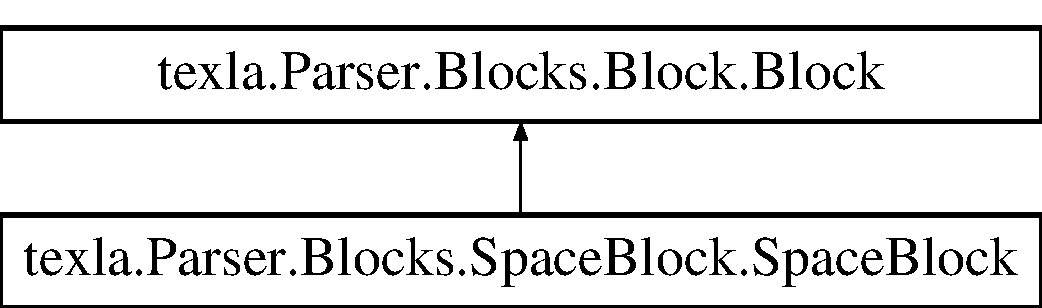
\includegraphics[height=2.000000cm]{classtexla_1_1Parser_1_1Blocks_1_1SpaceBlock_1_1SpaceBlock}
\end{center}
\end{figure}
\subsection*{Public Member Functions}
\begin{DoxyCompactItemize}
\item 
\hypertarget{classtexla_1_1Parser_1_1Blocks_1_1SpaceBlock_1_1SpaceBlock_a0e86fa42c902a08313373babfa01f35d}{}\label{classtexla_1_1Parser_1_1Blocks_1_1SpaceBlock_1_1SpaceBlock_a0e86fa42c902a08313373babfa01f35d} 
def {\bfseries \+\_\+\+\_\+init\+\_\+\+\_\+} (self, space\+\_\+type, length, parent\+\_\+block)
\end{DoxyCompactItemize}
\subsection*{Static Public Member Functions}
\begin{DoxyCompactItemize}
\item 
\hypertarget{classtexla_1_1Parser_1_1Blocks_1_1SpaceBlock_1_1SpaceBlock_af8d4de786d3160a00f25446ccf00adf7}{}\label{classtexla_1_1Parser_1_1Blocks_1_1SpaceBlock_1_1SpaceBlock_af8d4de786d3160a00f25446ccf00adf7} 
def {\bfseries parse} (parser, tex, parent\+\_\+block, params)
\end{DoxyCompactItemize}
\subsection*{Additional Inherited Members}


\subsection{Detailed Description}
\begin{DoxyVerb}This class gives you the possibility to
    put a vertical or horizontal space of the
    length you want\end{DoxyVerb}
 

The documentation for this class was generated from the following file\+:\begin{DoxyCompactItemize}
\item 
texla/\+Parser/\+Blocks/Space\+Block.\+py\end{DoxyCompactItemize}

\hypertarget{classtexla_1_1Parser_1_1Blocks_1_1TextBlocks_1_1SpecialCharacterBlock}{}\section{texla.\+Parser.\+Blocks.\+Text\+Blocks.\+Special\+Character\+Block Class Reference}
\label{classtexla_1_1Parser_1_1Blocks_1_1TextBlocks_1_1SpecialCharacterBlock}\index{texla.\+Parser.\+Blocks.\+Text\+Blocks.\+Special\+Character\+Block@{texla.\+Parser.\+Blocks.\+Text\+Blocks.\+Special\+Character\+Block}}
Inheritance diagram for texla.\+Parser.\+Blocks.\+Text\+Blocks.\+Special\+Character\+Block\+:\begin{figure}[H]
\begin{center}
\leavevmode
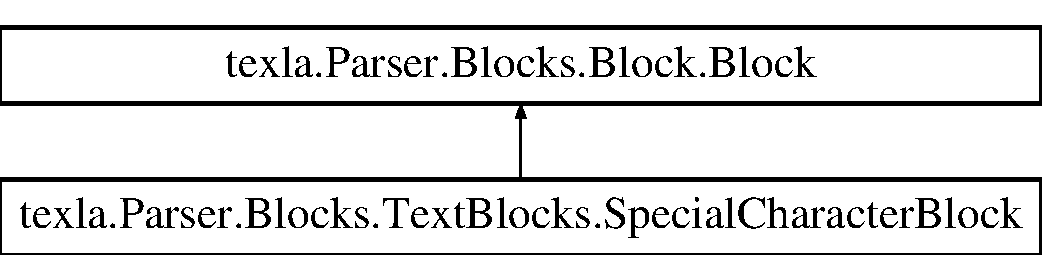
\includegraphics[height=2.000000cm]{classtexla_1_1Parser_1_1Blocks_1_1TextBlocks_1_1SpecialCharacterBlock}
\end{center}
\end{figure}
\subsection*{Public Member Functions}
\begin{DoxyCompactItemize}
\item 
\hypertarget{classtexla_1_1Parser_1_1Blocks_1_1TextBlocks_1_1SpecialCharacterBlock_ac516c028be490e1d7847b444f01d4535}{}\label{classtexla_1_1Parser_1_1Blocks_1_1TextBlocks_1_1SpecialCharacterBlock_ac516c028be490e1d7847b444f01d4535} 
def {\bfseries parse} (parser, tex, parent\+\_\+block, params)
\item 
\hypertarget{classtexla_1_1Parser_1_1Blocks_1_1TextBlocks_1_1SpecialCharacterBlock_a604dc98797d6f269ab5c40612be08bec}{}\label{classtexla_1_1Parser_1_1Blocks_1_1TextBlocks_1_1SpecialCharacterBlock_a604dc98797d6f269ab5c40612be08bec} 
def {\bfseries \+\_\+\+\_\+init\+\_\+\+\_\+} (self, char, parent\+\_\+block)
\end{DoxyCompactItemize}
\subsection*{Additional Inherited Members}


The documentation for this class was generated from the following file\+:\begin{DoxyCompactItemize}
\item 
texla/\+Parser/\+Blocks/Text\+Blocks.\+py\end{DoxyCompactItemize}

\hypertarget{classtexla_1_1Parser_1_1Blocks_1_1TabularBlocks_1_1TabularBlock}{}\section{texla.\+Parser.\+Blocks.\+Tabular\+Blocks.\+Tabular\+Block Class Reference}
\label{classtexla_1_1Parser_1_1Blocks_1_1TabularBlocks_1_1TabularBlock}\index{texla.\+Parser.\+Blocks.\+Tabular\+Blocks.\+Tabular\+Block@{texla.\+Parser.\+Blocks.\+Tabular\+Blocks.\+Tabular\+Block}}
Inheritance diagram for texla.\+Parser.\+Blocks.\+Tabular\+Blocks.\+Tabular\+Block\+:\begin{figure}[H]
\begin{center}
\leavevmode
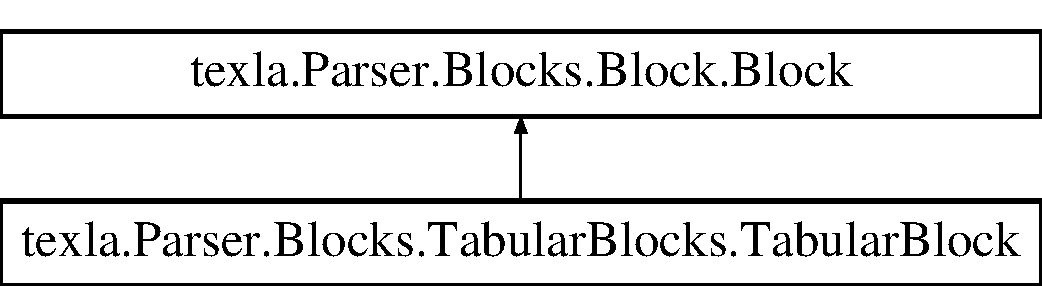
\includegraphics[height=2.000000cm]{classtexla_1_1Parser_1_1Blocks_1_1TabularBlocks_1_1TabularBlock}
\end{center}
\end{figure}
\subsection*{Public Member Functions}
\begin{DoxyCompactItemize}
\item 
\hypertarget{classtexla_1_1Parser_1_1Blocks_1_1TabularBlocks_1_1TabularBlock_aabc52fe3898e0309fbc223265f27e816}{}\label{classtexla_1_1Parser_1_1Blocks_1_1TabularBlocks_1_1TabularBlock_aabc52fe3898e0309fbc223265f27e816} 
def {\bfseries \+\_\+\+\_\+init\+\_\+\+\_\+} (self, pos, spec, parent\+\_\+block)
\end{DoxyCompactItemize}
\subsection*{Static Public Member Functions}
\begin{DoxyCompactItemize}
\item 
\hypertarget{classtexla_1_1Parser_1_1Blocks_1_1TabularBlocks_1_1TabularBlock_ac4888029c6b1d87571d8e2bd9c9230cc}{}\label{classtexla_1_1Parser_1_1Blocks_1_1TabularBlocks_1_1TabularBlock_ac4888029c6b1d87571d8e2bd9c9230cc} 
def {\bfseries parse} (parser, tex, parent\+\_\+block, params)
\item 
def \hyperlink{classtexla_1_1Parser_1_1Blocks_1_1TabularBlocks_1_1TabularBlock_a44ef251d20c1365275ab9ffeda057f69}{get\+\_\+spec\+\_\+dictionary} (spec)
\end{DoxyCompactItemize}
\subsection*{Public Attributes}
\begin{DoxyCompactItemize}
\item 
\hypertarget{classtexla_1_1Parser_1_1Blocks_1_1TabularBlocks_1_1TabularBlock_a111dd079fecc68bde1e245608fb10c7f}{}\label{classtexla_1_1Parser_1_1Blocks_1_1TabularBlocks_1_1TabularBlock_a111dd079fecc68bde1e245608fb10c7f} 
{\bfseries pos}
\end{DoxyCompactItemize}


\subsection{Member Function Documentation}
\hypertarget{classtexla_1_1Parser_1_1Blocks_1_1TabularBlocks_1_1TabularBlock_a44ef251d20c1365275ab9ffeda057f69}{}\label{classtexla_1_1Parser_1_1Blocks_1_1TabularBlocks_1_1TabularBlock_a44ef251d20c1365275ab9ffeda057f69} 
\index{texla\+::\+Parser\+::\+Blocks\+::\+Tabular\+Blocks\+::\+Tabular\+Block@{texla\+::\+Parser\+::\+Blocks\+::\+Tabular\+Blocks\+::\+Tabular\+Block}!get\+\_\+spec\+\_\+dictionary@{get\+\_\+spec\+\_\+dictionary}}
\index{get\+\_\+spec\+\_\+dictionary@{get\+\_\+spec\+\_\+dictionary}!texla\+::\+Parser\+::\+Blocks\+::\+Tabular\+Blocks\+::\+Tabular\+Block@{texla\+::\+Parser\+::\+Blocks\+::\+Tabular\+Blocks\+::\+Tabular\+Block}}
\subsubsection{\texorpdfstring{get\+\_\+spec\+\_\+dictionary()}{get\_spec\_dictionary()}}
{\footnotesize\ttfamily def texla.\+Parser.\+Blocks.\+Tabular\+Blocks.\+Tabular\+Block.\+get\+\_\+spec\+\_\+dictionary (\begin{DoxyParamCaption}\item[{}]{spec }\end{DoxyParamCaption})\hspace{0.3cm}{\ttfamily [static]}}

\begin{DoxyVerb}This function create  a list for the spec of the tables
\end{DoxyVerb}
 

The documentation for this class was generated from the following file\+:\begin{DoxyCompactItemize}
\item 
texla/\+Parser/\+Blocks/Tabular\+Blocks.\+py\end{DoxyCompactItemize}

\hypertarget{classtexla_1_1Parser_1_1Blocks_1_1TextBlocks_1_1TextBlock}{}\section{texla.\+Parser.\+Blocks.\+Text\+Blocks.\+Text\+Block Class Reference}
\label{classtexla_1_1Parser_1_1Blocks_1_1TextBlocks_1_1TextBlock}\index{texla.\+Parser.\+Blocks.\+Text\+Blocks.\+Text\+Block@{texla.\+Parser.\+Blocks.\+Text\+Blocks.\+Text\+Block}}
Inheritance diagram for texla.\+Parser.\+Blocks.\+Text\+Blocks.\+Text\+Block\+:\begin{figure}[H]
\begin{center}
\leavevmode
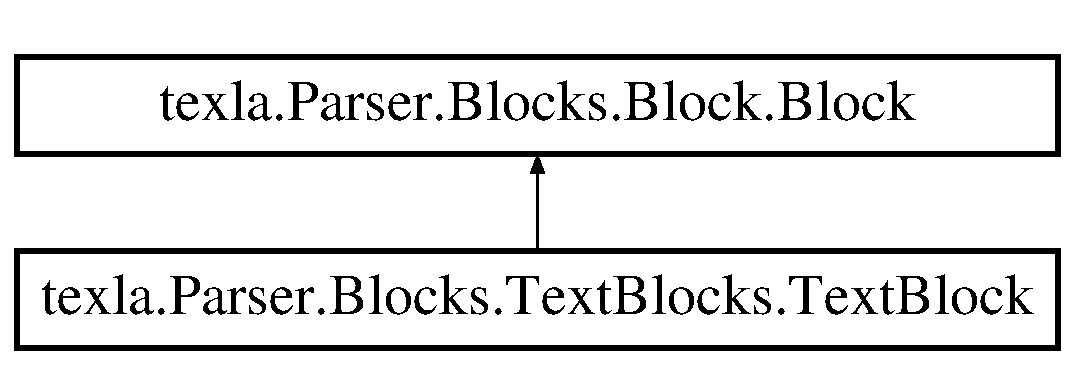
\includegraphics[height=2.000000cm]{classtexla_1_1Parser_1_1Blocks_1_1TextBlocks_1_1TextBlock}
\end{center}
\end{figure}
\subsection*{Public Member Functions}
\begin{DoxyCompactItemize}
\item 
def \hyperlink{classtexla_1_1Parser_1_1Blocks_1_1TextBlocks_1_1TextBlock_afc1b469142bce14bab40d102d42203f0}{\+\_\+\+\_\+init\+\_\+\+\_\+} (self, text, parent\+\_\+block)
\item 
\hypertarget{classtexla_1_1Parser_1_1Blocks_1_1TextBlocks_1_1TextBlock_ad878a924a1d956e00a1111396f77c261}{}\label{classtexla_1_1Parser_1_1Blocks_1_1TextBlocks_1_1TextBlock_ad878a924a1d956e00a1111396f77c261} 
def {\bfseries \+\_\+\+\_\+str\+\_\+\+\_\+} (self)
\end{DoxyCompactItemize}
\subsection*{Static Public Member Functions}
\begin{DoxyCompactItemize}
\item 
def \hyperlink{classtexla_1_1Parser_1_1Blocks_1_1TextBlocks_1_1TextBlock_a3a56fbfda7373ac5a103d5af52780b1a}{parse\+\_\+plain\+\_\+text} (parser, tex, parent\+\_\+block, params)
\item 
def \hyperlink{classtexla_1_1Parser_1_1Blocks_1_1TextBlocks_1_1TextBlock_a9abef4d8bec9802fe085eeb1e236f2fb}{fix\+\_\+text} (text)
\end{DoxyCompactItemize}
\subsection*{Additional Inherited Members}


\subsection{Constructor \& Destructor Documentation}
\hypertarget{classtexla_1_1Parser_1_1Blocks_1_1TextBlocks_1_1TextBlock_afc1b469142bce14bab40d102d42203f0}{}\label{classtexla_1_1Parser_1_1Blocks_1_1TextBlocks_1_1TextBlock_afc1b469142bce14bab40d102d42203f0} 
\index{texla\+::\+Parser\+::\+Blocks\+::\+Text\+Blocks\+::\+Text\+Block@{texla\+::\+Parser\+::\+Blocks\+::\+Text\+Blocks\+::\+Text\+Block}!\+\_\+\+\_\+init\+\_\+\+\_\+@{\+\_\+\+\_\+init\+\_\+\+\_\+}}
\index{\+\_\+\+\_\+init\+\_\+\+\_\+@{\+\_\+\+\_\+init\+\_\+\+\_\+}!texla\+::\+Parser\+::\+Blocks\+::\+Text\+Blocks\+::\+Text\+Block@{texla\+::\+Parser\+::\+Blocks\+::\+Text\+Blocks\+::\+Text\+Block}}
\subsubsection{\texorpdfstring{\+\_\+\+\_\+init\+\_\+\+\_\+()}{\_\_init\_\_()}}
{\footnotesize\ttfamily def texla.\+Parser.\+Blocks.\+Text\+Blocks.\+Text\+Block.\+\_\+\+\_\+init\+\_\+\+\_\+ (\begin{DoxyParamCaption}\item[{}]{self,  }\item[{}]{text,  }\item[{}]{parent\+\_\+block }\end{DoxyParamCaption})}

\begin{DoxyVerb}Constructor for text:
-text: string:
\end{DoxyVerb}
 

\subsection{Member Function Documentation}
\hypertarget{classtexla_1_1Parser_1_1Blocks_1_1TextBlocks_1_1TextBlock_a9abef4d8bec9802fe085eeb1e236f2fb}{}\label{classtexla_1_1Parser_1_1Blocks_1_1TextBlocks_1_1TextBlock_a9abef4d8bec9802fe085eeb1e236f2fb} 
\index{texla\+::\+Parser\+::\+Blocks\+::\+Text\+Blocks\+::\+Text\+Block@{texla\+::\+Parser\+::\+Blocks\+::\+Text\+Blocks\+::\+Text\+Block}!fix\+\_\+text@{fix\+\_\+text}}
\index{fix\+\_\+text@{fix\+\_\+text}!texla\+::\+Parser\+::\+Blocks\+::\+Text\+Blocks\+::\+Text\+Block@{texla\+::\+Parser\+::\+Blocks\+::\+Text\+Blocks\+::\+Text\+Block}}
\subsubsection{\texorpdfstring{fix\+\_\+text()}{fix\_text()}}
{\footnotesize\ttfamily def texla.\+Parser.\+Blocks.\+Text\+Blocks.\+Text\+Block.\+fix\+\_\+text (\begin{DoxyParamCaption}\item[{}]{text }\end{DoxyParamCaption})\hspace{0.3cm}{\ttfamily [static]}}

\begin{DoxyVerb}Function that removes useless spaces from text\end{DoxyVerb}
 \hypertarget{classtexla_1_1Parser_1_1Blocks_1_1TextBlocks_1_1TextBlock_a3a56fbfda7373ac5a103d5af52780b1a}{}\label{classtexla_1_1Parser_1_1Blocks_1_1TextBlocks_1_1TextBlock_a3a56fbfda7373ac5a103d5af52780b1a} 
\index{texla\+::\+Parser\+::\+Blocks\+::\+Text\+Blocks\+::\+Text\+Block@{texla\+::\+Parser\+::\+Blocks\+::\+Text\+Blocks\+::\+Text\+Block}!parse\+\_\+plain\+\_\+text@{parse\+\_\+plain\+\_\+text}}
\index{parse\+\_\+plain\+\_\+text@{parse\+\_\+plain\+\_\+text}!texla\+::\+Parser\+::\+Blocks\+::\+Text\+Blocks\+::\+Text\+Block@{texla\+::\+Parser\+::\+Blocks\+::\+Text\+Blocks\+::\+Text\+Block}}
\subsubsection{\texorpdfstring{parse\+\_\+plain\+\_\+text()}{parse\_plain\_text()}}
{\footnotesize\ttfamily def texla.\+Parser.\+Blocks.\+Text\+Blocks.\+Text\+Block.\+parse\+\_\+plain\+\_\+text (\begin{DoxyParamCaption}\item[{}]{parser,  }\item[{}]{tex,  }\item[{}]{parent\+\_\+block,  }\item[{}]{params }\end{DoxyParamCaption})\hspace{0.3cm}{\ttfamily [static]}}

\begin{DoxyVerb}Plain text is seen as and env. It has only to return
the block\end{DoxyVerb}
 

The documentation for this class was generated from the following file\+:\begin{DoxyCompactItemize}
\item 
texla/\+Parser/\+Blocks/Text\+Blocks.\+py\end{DoxyCompactItemize}

\hypertarget{classtexla_1_1Parser_1_1Blocks_1_1TheoremBlocks_1_1Theorem}{}\section{texla.\+Parser.\+Blocks.\+Theorem\+Blocks.\+Theorem Class Reference}
\label{classtexla_1_1Parser_1_1Blocks_1_1TheoremBlocks_1_1Theorem}\index{texla.\+Parser.\+Blocks.\+Theorem\+Blocks.\+Theorem@{texla.\+Parser.\+Blocks.\+Theorem\+Blocks.\+Theorem}}
\subsection*{Public Member Functions}
\begin{DoxyCompactItemize}
\item 
\hypertarget{classtexla_1_1Parser_1_1Blocks_1_1TheoremBlocks_1_1Theorem_a4ed44a6bbcb1d14b236fb469d6a524de}{}\label{classtexla_1_1Parser_1_1Blocks_1_1TheoremBlocks_1_1Theorem_a4ed44a6bbcb1d14b236fb469d6a524de} 
def {\bfseries \+\_\+\+\_\+init\+\_\+\+\_\+} (self, th\+\_\+type, definition, star, counter, numberby, title=\textquotesingle{}\textquotesingle{})
\end{DoxyCompactItemize}
\subsection*{Public Attributes}
\begin{DoxyCompactItemize}
\item 
\hypertarget{classtexla_1_1Parser_1_1Blocks_1_1TheoremBlocks_1_1Theorem_ae3f7f0082b83aba3f2d669201291d7c3}{}\label{classtexla_1_1Parser_1_1Blocks_1_1TheoremBlocks_1_1Theorem_ae3f7f0082b83aba3f2d669201291d7c3} 
{\bfseries th\+\_\+type}
\item 
\hypertarget{classtexla_1_1Parser_1_1Blocks_1_1TheoremBlocks_1_1Theorem_a21cee7a1b1d111f47545454527368e7d}{}\label{classtexla_1_1Parser_1_1Blocks_1_1TheoremBlocks_1_1Theorem_a21cee7a1b1d111f47545454527368e7d} 
{\bfseries definition}
\item 
\hypertarget{classtexla_1_1Parser_1_1Blocks_1_1TheoremBlocks_1_1Theorem_a0bc1b6699fcaa6b39a036e2619c1e1d5}{}\label{classtexla_1_1Parser_1_1Blocks_1_1TheoremBlocks_1_1Theorem_a0bc1b6699fcaa6b39a036e2619c1e1d5} 
{\bfseries star}
\item 
\hypertarget{classtexla_1_1Parser_1_1Blocks_1_1TheoremBlocks_1_1Theorem_a8eafc4fe56186b7b1dad639f4e14914d}{}\label{classtexla_1_1Parser_1_1Blocks_1_1TheoremBlocks_1_1Theorem_a8eafc4fe56186b7b1dad639f4e14914d} 
{\bfseries counter}
\item 
\hypertarget{classtexla_1_1Parser_1_1Blocks_1_1TheoremBlocks_1_1Theorem_a3c49decf41fd5931245adb4d24e05c0c}{}\label{classtexla_1_1Parser_1_1Blocks_1_1TheoremBlocks_1_1Theorem_a3c49decf41fd5931245adb4d24e05c0c} 
{\bfseries numberby}
\item 
\hypertarget{classtexla_1_1Parser_1_1Blocks_1_1TheoremBlocks_1_1Theorem_a9f3690b53ea81ce58e43fc5fef8af354}{}\label{classtexla_1_1Parser_1_1Blocks_1_1TheoremBlocks_1_1Theorem_a9f3690b53ea81ce58e43fc5fef8af354} 
{\bfseries title}
\end{DoxyCompactItemize}


\subsection{Detailed Description}
\begin{DoxyVerb}This object represents a theorem defined
by the user\end{DoxyVerb}
 

The documentation for this class was generated from the following file\+:\begin{DoxyCompactItemize}
\item 
texla/\+Parser/\+Blocks/Theorem\+Blocks.\+py\end{DoxyCompactItemize}

\hypertarget{classtexla_1_1PageTree_1_1TheoremsManager_1_1Theorem}{}\section{texla.\+Page\+Tree.\+Theorems\+Manager.\+Theorem Class Reference}
\label{classtexla_1_1PageTree_1_1TheoremsManager_1_1Theorem}\index{texla.\+Page\+Tree.\+Theorems\+Manager.\+Theorem@{texla.\+Page\+Tree.\+Theorems\+Manager.\+Theorem}}
\subsection*{Public Member Functions}
\begin{DoxyCompactItemize}
\item 
\hypertarget{classtexla_1_1PageTree_1_1TheoremsManager_1_1Theorem_abf229dbbda7151f0975d4e4ffb46e779}{}\label{classtexla_1_1PageTree_1_1TheoremsManager_1_1Theorem_abf229dbbda7151f0975d4e4ffb46e779} 
def {\bfseries \+\_\+\+\_\+init\+\_\+\+\_\+} (self, id, page, th\+\_\+type)
\item 
def \hyperlink{classtexla_1_1PageTree_1_1TheoremsManager_1_1Theorem_a95c04605568b92d092b5c30b1538e318}{fix\+Number} (self, number)
\item 
def \hyperlink{classtexla_1_1PageTree_1_1TheoremsManager_1_1Theorem_a894e4a4e21490eab706503be1c65c6d9}{fix\+Url} (self)
\item 
\hypertarget{classtexla_1_1PageTree_1_1TheoremsManager_1_1Theorem_aa0ee71e9d0390c7d35c25521d5e95f84}{}\label{classtexla_1_1PageTree_1_1TheoremsManager_1_1Theorem_aa0ee71e9d0390c7d35c25521d5e95f84} 
def {\bfseries \+\_\+\+\_\+str\+\_\+\+\_\+} (self)
\end{DoxyCompactItemize}
\subsection*{Public Attributes}
\begin{DoxyCompactItemize}
\item 
\hypertarget{classtexla_1_1PageTree_1_1TheoremsManager_1_1Theorem_ae4801c9a2372be00c472bc293f7bd312}{}\label{classtexla_1_1PageTree_1_1TheoremsManager_1_1Theorem_ae4801c9a2372be00c472bc293f7bd312} 
{\bfseries id}
\item 
\hypertarget{classtexla_1_1PageTree_1_1TheoremsManager_1_1Theorem_a6e0dbaa9c063f72d6d62cc6bbdadb945}{}\label{classtexla_1_1PageTree_1_1TheoremsManager_1_1Theorem_a6e0dbaa9c063f72d6d62cc6bbdadb945} 
{\bfseries page}
\item 
\hypertarget{classtexla_1_1PageTree_1_1TheoremsManager_1_1Theorem_a9e3436a8dc4af492ee8431928bcca358}{}\label{classtexla_1_1PageTree_1_1TheoremsManager_1_1Theorem_a9e3436a8dc4af492ee8431928bcca358} 
{\bfseries text}
\item 
\hypertarget{classtexla_1_1PageTree_1_1TheoremsManager_1_1Theorem_aaf9edaa707fa727934206afd285cfc00}{}\label{classtexla_1_1PageTree_1_1TheoremsManager_1_1Theorem_aaf9edaa707fa727934206afd285cfc00} 
{\bfseries th\+\_\+type}
\item 
\hypertarget{classtexla_1_1PageTree_1_1TheoremsManager_1_1Theorem_ac634737d4833043e63bffea7866451fd}{}\label{classtexla_1_1PageTree_1_1TheoremsManager_1_1Theorem_ac634737d4833043e63bffea7866451fd} 
{\bfseries number}
\item 
\hypertarget{classtexla_1_1PageTree_1_1TheoremsManager_1_1Theorem_ada861276b37b38190fbed67e25145e6c}{}\label{classtexla_1_1PageTree_1_1TheoremsManager_1_1Theorem_ada861276b37b38190fbed67e25145e6c} 
{\bfseries title}
\item 
\hypertarget{classtexla_1_1PageTree_1_1TheoremsManager_1_1Theorem_a33f5654cfd0f472b558378d2ddce0c14}{}\label{classtexla_1_1PageTree_1_1TheoremsManager_1_1Theorem_a33f5654cfd0f472b558378d2ddce0c14} 
{\bfseries url}
\end{DoxyCompactItemize}


\subsection{Member Function Documentation}
\hypertarget{classtexla_1_1PageTree_1_1TheoremsManager_1_1Theorem_a95c04605568b92d092b5c30b1538e318}{}\label{classtexla_1_1PageTree_1_1TheoremsManager_1_1Theorem_a95c04605568b92d092b5c30b1538e318} 
\index{texla\+::\+Page\+Tree\+::\+Theorems\+Manager\+::\+Theorem@{texla\+::\+Page\+Tree\+::\+Theorems\+Manager\+::\+Theorem}!fix\+Number@{fix\+Number}}
\index{fix\+Number@{fix\+Number}!texla\+::\+Page\+Tree\+::\+Theorems\+Manager\+::\+Theorem@{texla\+::\+Page\+Tree\+::\+Theorems\+Manager\+::\+Theorem}}
\subsubsection{\texorpdfstring{fix\+Number()}{fixNumber()}}
{\footnotesize\ttfamily def texla.\+Page\+Tree.\+Theorems\+Manager.\+Theorem.\+fix\+Number (\begin{DoxyParamCaption}\item[{}]{self,  }\item[{}]{number }\end{DoxyParamCaption})}

\begin{DoxyVerb}This method fix the number of the theorem
inside its page text replacing the string {{thnum:id}}.
The number is also appended to the title\end{DoxyVerb}
 \hypertarget{classtexla_1_1PageTree_1_1TheoremsManager_1_1Theorem_a894e4a4e21490eab706503be1c65c6d9}{}\label{classtexla_1_1PageTree_1_1TheoremsManager_1_1Theorem_a894e4a4e21490eab706503be1c65c6d9} 
\index{texla\+::\+Page\+Tree\+::\+Theorems\+Manager\+::\+Theorem@{texla\+::\+Page\+Tree\+::\+Theorems\+Manager\+::\+Theorem}!fix\+Url@{fix\+Url}}
\index{fix\+Url@{fix\+Url}!texla\+::\+Page\+Tree\+::\+Theorems\+Manager\+::\+Theorem@{texla\+::\+Page\+Tree\+::\+Theorems\+Manager\+::\+Theorem}}
\subsubsection{\texorpdfstring{fix\+Url()}{fixUrl()}}
{\footnotesize\ttfamily def texla.\+Page\+Tree.\+Theorems\+Manager.\+Theorem.\+fix\+Url (\begin{DoxyParamCaption}\item[{}]{self }\end{DoxyParamCaption})}

\begin{DoxyVerb}The theorem url is setted to the page url.
N.B.: to be called after pages' urls fixing\end{DoxyVerb}
 

The documentation for this class was generated from the following file\+:\begin{DoxyCompactItemize}
\item 
texla/\+Page\+Tree/Theorems\+Manager.\+py\end{DoxyCompactItemize}

\hypertarget{classtexla_1_1Parser_1_1Blocks_1_1TheoremBlocks_1_1TheoremBlock}{}\section{texla.\+Parser.\+Blocks.\+Theorem\+Blocks.\+Theorem\+Block Class Reference}
\label{classtexla_1_1Parser_1_1Blocks_1_1TheoremBlocks_1_1TheoremBlock}\index{texla.\+Parser.\+Blocks.\+Theorem\+Blocks.\+Theorem\+Block@{texla.\+Parser.\+Blocks.\+Theorem\+Blocks.\+Theorem\+Block}}
Inheritance diagram for texla.\+Parser.\+Blocks.\+Theorem\+Blocks.\+Theorem\+Block\+:\begin{figure}[H]
\begin{center}
\leavevmode
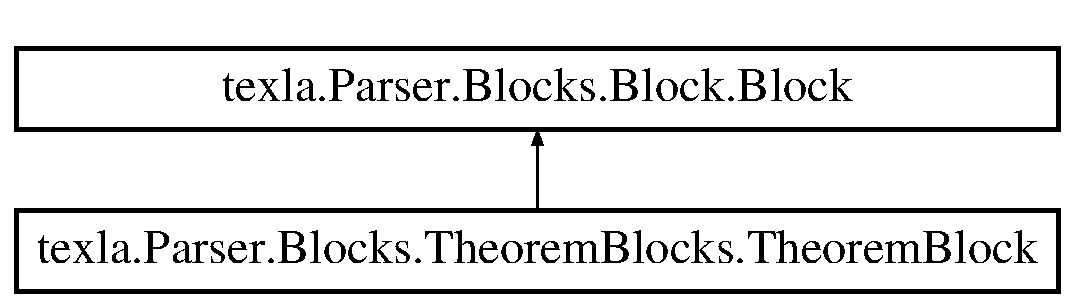
\includegraphics[height=2.000000cm]{classtexla_1_1Parser_1_1Blocks_1_1TheoremBlocks_1_1TheoremBlock}
\end{center}
\end{figure}
\subsection*{Public Member Functions}
\begin{DoxyCompactItemize}
\item 
\hypertarget{classtexla_1_1Parser_1_1Blocks_1_1TheoremBlocks_1_1TheoremBlock_a90f4759fea5d972d2b10940bf23c930a}{}\label{classtexla_1_1Parser_1_1Blocks_1_1TheoremBlocks_1_1TheoremBlock_a90f4759fea5d972d2b10940bf23c930a} 
def {\bfseries \+\_\+\+\_\+init\+\_\+\+\_\+} (self, theorem, title, content, parent\+\_\+block)
\end{DoxyCompactItemize}
\subsection*{Static Public Member Functions}
\begin{DoxyCompactItemize}
\item 
\hypertarget{classtexla_1_1Parser_1_1Blocks_1_1TheoremBlocks_1_1TheoremBlock_ac08408210195d57c98e8c8d5712f08ad}{}\label{classtexla_1_1Parser_1_1Blocks_1_1TheoremBlocks_1_1TheoremBlock_ac08408210195d57c98e8c8d5712f08ad} 
def {\bfseries parse} (parser, tex, parent\+\_\+block, params)
\end{DoxyCompactItemize}
\subsection*{Public Attributes}
\begin{DoxyCompactItemize}
\item 
\hypertarget{classtexla_1_1Parser_1_1Blocks_1_1TheoremBlocks_1_1TheoremBlock_aea09c62cdfb8b60f7408be067f22277a}{}\label{classtexla_1_1Parser_1_1Blocks_1_1TheoremBlocks_1_1TheoremBlock_aea09c62cdfb8b60f7408be067f22277a} 
{\bfseries theorem}
\item 
\hypertarget{classtexla_1_1Parser_1_1Blocks_1_1TheoremBlocks_1_1TheoremBlock_a3f93bd7c5f34eddf7bd0913e2d579dd6}{}\label{classtexla_1_1Parser_1_1Blocks_1_1TheoremBlocks_1_1TheoremBlock_a3f93bd7c5f34eddf7bd0913e2d579dd6} 
{\bfseries th\+\_\+type}
\end{DoxyCompactItemize}


\subsection{Detailed Description}
\begin{DoxyVerb}The theorem block represts a theorem.
The different type of theorems defined by the
writer are preparsed and put into parser_theorems.
The TheoremBlock saves the found theorem with its
title and theorem type object \end{DoxyVerb}
 

The documentation for this class was generated from the following file\+:\begin{DoxyCompactItemize}
\item 
texla/\+Parser/\+Blocks/Theorem\+Blocks.\+py\end{DoxyCompactItemize}

\hypertarget{classtexla_1_1PageTree_1_1TheoremsManager_1_1TheoremsManager}{}\section{texla.\+Page\+Tree.\+Theorems\+Manager.\+Theorems\+Manager Class Reference}
\label{classtexla_1_1PageTree_1_1TheoremsManager_1_1TheoremsManager}\index{texla.\+Page\+Tree.\+Theorems\+Manager.\+Theorems\+Manager@{texla.\+Page\+Tree.\+Theorems\+Manager.\+Theorems\+Manager}}
\subsection*{Public Member Functions}
\begin{DoxyCompactItemize}
\item 
\hypertarget{classtexla_1_1PageTree_1_1TheoremsManager_1_1TheoremsManager_a838c2b4785f4a9e1ba3c7dbc67135f11}{}\label{classtexla_1_1PageTree_1_1TheoremsManager_1_1TheoremsManager_a838c2b4785f4a9e1ba3c7dbc67135f11} 
def {\bfseries \+\_\+\+\_\+init\+\_\+\+\_\+} (self, pages\+\_\+dict)
\item 
\hypertarget{classtexla_1_1PageTree_1_1TheoremsManager_1_1TheoremsManager_a6c07b258a97c0e2f9fd959b63bac0151}{}\label{classtexla_1_1PageTree_1_1TheoremsManager_1_1TheoremsManager_a6c07b258a97c0e2f9fd959b63bac0151} 
def {\bfseries add\+Theorem} (self, theorem)
\item 
def \hyperlink{classtexla_1_1PageTree_1_1TheoremsManager_1_1TheoremsManager_a31188ef920568ca338e846b292c1e0b1}{move\+\_\+theorems\+\_\+page} (self, oldpage, newpage)
\item 
def \hyperlink{classtexla_1_1PageTree_1_1TheoremsManager_1_1TheoremsManager_a399fc28cf03a96352c6136a850cd46b9}{fix\+\_\+theorems} (self)
\item 
\hypertarget{classtexla_1_1PageTree_1_1TheoremsManager_1_1TheoremsManager_a5921ce72c90d386d07dc04ebdda83a5b}{}\label{classtexla_1_1PageTree_1_1TheoremsManager_1_1TheoremsManager_a5921ce72c90d386d07dc04ebdda83a5b} 
def {\bfseries get\+\_\+subpages\+\_\+ordered} (self, page)
\end{DoxyCompactItemize}
\subsection*{Public Attributes}
\begin{DoxyCompactItemize}
\item 
\hypertarget{classtexla_1_1PageTree_1_1TheoremsManager_1_1TheoremsManager_afb35ab75facdff4f0e5d92e110a38fe9}{}\label{classtexla_1_1PageTree_1_1TheoremsManager_1_1TheoremsManager_afb35ab75facdff4f0e5d92e110a38fe9} 
{\bfseries pages}
\item 
\hypertarget{classtexla_1_1PageTree_1_1TheoremsManager_1_1TheoremsManager_a46e115caef1a718e23db1d766c249856}{}\label{classtexla_1_1PageTree_1_1TheoremsManager_1_1TheoremsManager_a46e115caef1a718e23db1d766c249856} 
{\bfseries pages\+\_\+ths}
\end{DoxyCompactItemize}


\subsection{Member Function Documentation}
\hypertarget{classtexla_1_1PageTree_1_1TheoremsManager_1_1TheoremsManager_a399fc28cf03a96352c6136a850cd46b9}{}\label{classtexla_1_1PageTree_1_1TheoremsManager_1_1TheoremsManager_a399fc28cf03a96352c6136a850cd46b9} 
\index{texla\+::\+Page\+Tree\+::\+Theorems\+Manager\+::\+Theorems\+Manager@{texla\+::\+Page\+Tree\+::\+Theorems\+Manager\+::\+Theorems\+Manager}!fix\+\_\+theorems@{fix\+\_\+theorems}}
\index{fix\+\_\+theorems@{fix\+\_\+theorems}!texla\+::\+Page\+Tree\+::\+Theorems\+Manager\+::\+Theorems\+Manager@{texla\+::\+Page\+Tree\+::\+Theorems\+Manager\+::\+Theorems\+Manager}}
\subsubsection{\texorpdfstring{fix\+\_\+theorems()}{fix\_theorems()}}
{\footnotesize\ttfamily def texla.\+Page\+Tree.\+Theorems\+Manager.\+Theorems\+Manager.\+fix\+\_\+theorems (\begin{DoxyParamCaption}\item[{}]{self }\end{DoxyParamCaption})}

\begin{DoxyVerb}This function fixes the theorems calculating their
number and substituing it the placeholder in the text.
Moreover it fixes the data needed by the label manager.\end{DoxyVerb}
 \hypertarget{classtexla_1_1PageTree_1_1TheoremsManager_1_1TheoremsManager_a31188ef920568ca338e846b292c1e0b1}{}\label{classtexla_1_1PageTree_1_1TheoremsManager_1_1TheoremsManager_a31188ef920568ca338e846b292c1e0b1} 
\index{texla\+::\+Page\+Tree\+::\+Theorems\+Manager\+::\+Theorems\+Manager@{texla\+::\+Page\+Tree\+::\+Theorems\+Manager\+::\+Theorems\+Manager}!move\+\_\+theorems\+\_\+page@{move\+\_\+theorems\+\_\+page}}
\index{move\+\_\+theorems\+\_\+page@{move\+\_\+theorems\+\_\+page}!texla\+::\+Page\+Tree\+::\+Theorems\+Manager\+::\+Theorems\+Manager@{texla\+::\+Page\+Tree\+::\+Theorems\+Manager\+::\+Theorems\+Manager}}
\subsubsection{\texorpdfstring{move\+\_\+theorems\+\_\+page()}{move\_theorems\_page()}}
{\footnotesize\ttfamily def texla.\+Page\+Tree.\+Theorems\+Manager.\+Theorems\+Manager.\+move\+\_\+theorems\+\_\+page (\begin{DoxyParamCaption}\item[{}]{self,  }\item[{}]{oldpage,  }\item[{}]{newpage }\end{DoxyParamCaption})}

\begin{DoxyVerb}This function moves a theorem to a different page
to maintain the right anchor in case of moved page.\end{DoxyVerb}
 

The documentation for this class was generated from the following file\+:\begin{DoxyCompactItemize}
\item 
texla/\+Page\+Tree/Theorems\+Manager.\+py\end{DoxyCompactItemize}

\hypertarget{classtexla_1_1Parser_1_1TreeExplorer_1_1TreeExplorer}{}\section{texla.\+Parser.\+Tree\+Explorer.\+Tree\+Explorer Class Reference}
\label{classtexla_1_1Parser_1_1TreeExplorer_1_1TreeExplorer}\index{texla.\+Parser.\+Tree\+Explorer.\+Tree\+Explorer@{texla.\+Parser.\+Tree\+Explorer.\+Tree\+Explorer}}
\subsection*{Public Member Functions}
\begin{DoxyCompactItemize}
\item 
def \hyperlink{classtexla_1_1Parser_1_1TreeExplorer_1_1TreeExplorer_a02f877a37a394d2a471cab047dc04529}{\+\_\+\+\_\+init\+\_\+\+\_\+} (self, root\+\_\+block)
\item 
def \hyperlink{classtexla_1_1Parser_1_1TreeExplorer_1_1TreeExplorer_a07c509d8c1ce6695e1e343b722b19dbe}{register\+\_\+blocks} (self, blocks)
\item 
def \hyperlink{classtexla_1_1Parser_1_1TreeExplorer_1_1TreeExplorer_a920a80c8a3e38a5144641b688938ad8d}{update\+\_\+blocks\+\_\+register} (self)
\item 
def \hyperlink{classtexla_1_1Parser_1_1TreeExplorer_1_1TreeExplorer_ad948e5828a35215fa58ec9ba7e194e7e}{get\+\_\+parents\+\_\+list} (self, block)
\item 
\hypertarget{classtexla_1_1Parser_1_1TreeExplorer_1_1TreeExplorer_a9dce5eba74c14d0adc0586665bc1119a}{}\label{classtexla_1_1Parser_1_1TreeExplorer_1_1TreeExplorer_a9dce5eba74c14d0adc0586665bc1119a} 
def {\bfseries get\+\_\+parents\+\_\+list\+\_\+ids} (self, block)
\item 
\hypertarget{classtexla_1_1Parser_1_1TreeExplorer_1_1TreeExplorer_a26e9613885db6426e6ba450b747460fe}{}\label{classtexla_1_1Parser_1_1TreeExplorer_1_1TreeExplorer_a26e9613885db6426e6ba450b747460fe} 
def {\bfseries get\+\_\+block} (self, blockid)
\item 
def \hyperlink{classtexla_1_1Parser_1_1TreeExplorer_1_1TreeExplorer_a3fb88b30a1ed2a58cbb3e4c1099c7ddd}{print\+\_\+tree} (self, block, filter\+\_\+list=None)
\item 
def \hyperlink{classtexla_1_1Parser_1_1TreeExplorer_1_1TreeExplorer_a958b21268709209a935f718b6a7b8c3d}{print\+\_\+tree\+\_\+to\+\_\+blocks} (self, blocks)
\item 
\hypertarget{classtexla_1_1Parser_1_1TreeExplorer_1_1TreeExplorer_a576660a84acb13e5852d716ed6707278}{}\label{classtexla_1_1Parser_1_1TreeExplorer_1_1TreeExplorer_a576660a84acb13e5852d716ed6707278} 
def {\bfseries print\+\_\+tree\+\_\+to\+\_\+block} (self, block)
\end{DoxyCompactItemize}
\subsection*{Static Public Member Functions}
\begin{DoxyCompactItemize}
\item 
\hypertarget{classtexla_1_1Parser_1_1TreeExplorer_1_1TreeExplorer_a8502a4b4eea15fb192b65a4174627ba9}{}\label{classtexla_1_1Parser_1_1TreeExplorer_1_1TreeExplorer_a8502a4b4eea15fb192b65a4174627ba9} 
def {\bfseries create\+\_\+tree\+\_\+from\+\_\+children} (block)
\end{DoxyCompactItemize}
\subsection*{Public Attributes}
\begin{DoxyCompactItemize}
\item 
\hypertarget{classtexla_1_1Parser_1_1TreeExplorer_1_1TreeExplorer_a318bd6f70f7691ea7c0f49be6cb7ceb6}{}\label{classtexla_1_1Parser_1_1TreeExplorer_1_1TreeExplorer_a318bd6f70f7691ea7c0f49be6cb7ceb6} 
{\bfseries root\+\_\+block}
\item 
\hypertarget{classtexla_1_1Parser_1_1TreeExplorer_1_1TreeExplorer_a8ebbc7c21ef860caae95e9be5fb66821}{}\label{classtexla_1_1Parser_1_1TreeExplorer_1_1TreeExplorer_a8ebbc7c21ef860caae95e9be5fb66821} 
{\bfseries blocks}
\end{DoxyCompactItemize}


\subsection{Detailed Description}
\begin{DoxyVerb}The TreeExplorer class is an utility to navigate
and extract information from the tree of parsed blocks.
For example it is useful to extract the tree of the
parents of a block for debugging reasons. It is useful
also in rendering to localize blocks inside the document.
\end{DoxyVerb}
 

\subsection{Constructor \& Destructor Documentation}
\hypertarget{classtexla_1_1Parser_1_1TreeExplorer_1_1TreeExplorer_a02f877a37a394d2a471cab047dc04529}{}\label{classtexla_1_1Parser_1_1TreeExplorer_1_1TreeExplorer_a02f877a37a394d2a471cab047dc04529} 
\index{texla\+::\+Parser\+::\+Tree\+Explorer\+::\+Tree\+Explorer@{texla\+::\+Parser\+::\+Tree\+Explorer\+::\+Tree\+Explorer}!\+\_\+\+\_\+init\+\_\+\+\_\+@{\+\_\+\+\_\+init\+\_\+\+\_\+}}
\index{\+\_\+\+\_\+init\+\_\+\+\_\+@{\+\_\+\+\_\+init\+\_\+\+\_\+}!texla\+::\+Parser\+::\+Tree\+Explorer\+::\+Tree\+Explorer@{texla\+::\+Parser\+::\+Tree\+Explorer\+::\+Tree\+Explorer}}
\subsubsection{\texorpdfstring{\+\_\+\+\_\+init\+\_\+\+\_\+()}{\_\_init\_\_()}}
{\footnotesize\ttfamily def texla.\+Parser.\+Tree\+Explorer.\+Tree\+Explorer.\+\_\+\+\_\+init\+\_\+\+\_\+ (\begin{DoxyParamCaption}\item[{}]{self,  }\item[{}]{root\+\_\+block }\end{DoxyParamCaption})}

\begin{DoxyVerb}The constructor needs a root_block to
begin the tree\end{DoxyVerb}
 

\subsection{Member Function Documentation}
\hypertarget{classtexla_1_1Parser_1_1TreeExplorer_1_1TreeExplorer_ad948e5828a35215fa58ec9ba7e194e7e}{}\label{classtexla_1_1Parser_1_1TreeExplorer_1_1TreeExplorer_ad948e5828a35215fa58ec9ba7e194e7e} 
\index{texla\+::\+Parser\+::\+Tree\+Explorer\+::\+Tree\+Explorer@{texla\+::\+Parser\+::\+Tree\+Explorer\+::\+Tree\+Explorer}!get\+\_\+parents\+\_\+list@{get\+\_\+parents\+\_\+list}}
\index{get\+\_\+parents\+\_\+list@{get\+\_\+parents\+\_\+list}!texla\+::\+Parser\+::\+Tree\+Explorer\+::\+Tree\+Explorer@{texla\+::\+Parser\+::\+Tree\+Explorer\+::\+Tree\+Explorer}}
\subsubsection{\texorpdfstring{get\+\_\+parents\+\_\+list()}{get\_parents\_list()}}
{\footnotesize\ttfamily def texla.\+Parser.\+Tree\+Explorer.\+Tree\+Explorer.\+get\+\_\+parents\+\_\+list (\begin{DoxyParamCaption}\item[{}]{self,  }\item[{}]{block }\end{DoxyParamCaption})}

\begin{DoxyVerb}This method returns the list of the parent
blocks of the requested block\end{DoxyVerb}
 \hypertarget{classtexla_1_1Parser_1_1TreeExplorer_1_1TreeExplorer_a3fb88b30a1ed2a58cbb3e4c1099c7ddd}{}\label{classtexla_1_1Parser_1_1TreeExplorer_1_1TreeExplorer_a3fb88b30a1ed2a58cbb3e4c1099c7ddd} 
\index{texla\+::\+Parser\+::\+Tree\+Explorer\+::\+Tree\+Explorer@{texla\+::\+Parser\+::\+Tree\+Explorer\+::\+Tree\+Explorer}!print\+\_\+tree@{print\+\_\+tree}}
\index{print\+\_\+tree@{print\+\_\+tree}!texla\+::\+Parser\+::\+Tree\+Explorer\+::\+Tree\+Explorer@{texla\+::\+Parser\+::\+Tree\+Explorer\+::\+Tree\+Explorer}}
\subsubsection{\texorpdfstring{print\+\_\+tree()}{print\_tree()}}
{\footnotesize\ttfamily def texla.\+Parser.\+Tree\+Explorer.\+Tree\+Explorer.\+print\+\_\+tree (\begin{DoxyParamCaption}\item[{}]{self,  }\item[{}]{block,  }\item[{}]{filter\+\_\+list = {\ttfamily None} }\end{DoxyParamCaption})}

\begin{DoxyVerb}This methods prints a beautified tree starting
from block parameter and his children. If filter_list
is present only the block with the id in the list
are printed. It returns a list of output strings\end{DoxyVerb}
 \hypertarget{classtexla_1_1Parser_1_1TreeExplorer_1_1TreeExplorer_a958b21268709209a935f718b6a7b8c3d}{}\label{classtexla_1_1Parser_1_1TreeExplorer_1_1TreeExplorer_a958b21268709209a935f718b6a7b8c3d} 
\index{texla\+::\+Parser\+::\+Tree\+Explorer\+::\+Tree\+Explorer@{texla\+::\+Parser\+::\+Tree\+Explorer\+::\+Tree\+Explorer}!print\+\_\+tree\+\_\+to\+\_\+blocks@{print\+\_\+tree\+\_\+to\+\_\+blocks}}
\index{print\+\_\+tree\+\_\+to\+\_\+blocks@{print\+\_\+tree\+\_\+to\+\_\+blocks}!texla\+::\+Parser\+::\+Tree\+Explorer\+::\+Tree\+Explorer@{texla\+::\+Parser\+::\+Tree\+Explorer\+::\+Tree\+Explorer}}
\subsubsection{\texorpdfstring{print\+\_\+tree\+\_\+to\+\_\+blocks()}{print\_tree\_to\_blocks()}}
{\footnotesize\ttfamily def texla.\+Parser.\+Tree\+Explorer.\+Tree\+Explorer.\+print\+\_\+tree\+\_\+to\+\_\+blocks (\begin{DoxyParamCaption}\item[{}]{self,  }\item[{}]{blocks }\end{DoxyParamCaption})}

\begin{DoxyVerb}This methods print the tree of parents
of the list of blocks passed as parameter.
First of all it gets all the parents ids and
then prints the tree using the list as filter.\end{DoxyVerb}
 \hypertarget{classtexla_1_1Parser_1_1TreeExplorer_1_1TreeExplorer_a07c509d8c1ce6695e1e343b722b19dbe}{}\label{classtexla_1_1Parser_1_1TreeExplorer_1_1TreeExplorer_a07c509d8c1ce6695e1e343b722b19dbe} 
\index{texla\+::\+Parser\+::\+Tree\+Explorer\+::\+Tree\+Explorer@{texla\+::\+Parser\+::\+Tree\+Explorer\+::\+Tree\+Explorer}!register\+\_\+blocks@{register\+\_\+blocks}}
\index{register\+\_\+blocks@{register\+\_\+blocks}!texla\+::\+Parser\+::\+Tree\+Explorer\+::\+Tree\+Explorer@{texla\+::\+Parser\+::\+Tree\+Explorer\+::\+Tree\+Explorer}}
\subsubsection{\texorpdfstring{register\+\_\+blocks()}{register\_blocks()}}
{\footnotesize\ttfamily def texla.\+Parser.\+Tree\+Explorer.\+Tree\+Explorer.\+register\+\_\+blocks (\begin{DoxyParamCaption}\item[{}]{self,  }\item[{}]{blocks }\end{DoxyParamCaption})}

\begin{DoxyVerb}This methods reads all the blocks tree
from the root_block and created a dictionary
with id:block\end{DoxyVerb}
 \hypertarget{classtexla_1_1Parser_1_1TreeExplorer_1_1TreeExplorer_a920a80c8a3e38a5144641b688938ad8d}{}\label{classtexla_1_1Parser_1_1TreeExplorer_1_1TreeExplorer_a920a80c8a3e38a5144641b688938ad8d} 
\index{texla\+::\+Parser\+::\+Tree\+Explorer\+::\+Tree\+Explorer@{texla\+::\+Parser\+::\+Tree\+Explorer\+::\+Tree\+Explorer}!update\+\_\+blocks\+\_\+register@{update\+\_\+blocks\+\_\+register}}
\index{update\+\_\+blocks\+\_\+register@{update\+\_\+blocks\+\_\+register}!texla\+::\+Parser\+::\+Tree\+Explorer\+::\+Tree\+Explorer@{texla\+::\+Parser\+::\+Tree\+Explorer\+::\+Tree\+Explorer}}
\subsubsection{\texorpdfstring{update\+\_\+blocks\+\_\+register()}{update\_blocks\_register()}}
{\footnotesize\ttfamily def texla.\+Parser.\+Tree\+Explorer.\+Tree\+Explorer.\+update\+\_\+blocks\+\_\+register (\begin{DoxyParamCaption}\item[{}]{self }\end{DoxyParamCaption})}

\begin{DoxyVerb}This methods update the blocks' ids register
recalling register_blocks with the root_block\end{DoxyVerb}
 

The documentation for this class was generated from the following file\+:\begin{DoxyCompactItemize}
\item 
texla/\+Parser/Tree\+Explorer.\+py\end{DoxyCompactItemize}

\hypertarget{classtexla_1_1Parser_1_1Blocks_1_1VerbatimBlock_1_1VerbatimBlock}{}\section{texla.\+Parser.\+Blocks.\+Verbatim\+Block.\+Verbatim\+Block Class Reference}
\label{classtexla_1_1Parser_1_1Blocks_1_1VerbatimBlock_1_1VerbatimBlock}\index{texla.\+Parser.\+Blocks.\+Verbatim\+Block.\+Verbatim\+Block@{texla.\+Parser.\+Blocks.\+Verbatim\+Block.\+Verbatim\+Block}}
Inheritance diagram for texla.\+Parser.\+Blocks.\+Verbatim\+Block.\+Verbatim\+Block\+:\begin{figure}[H]
\begin{center}
\leavevmode
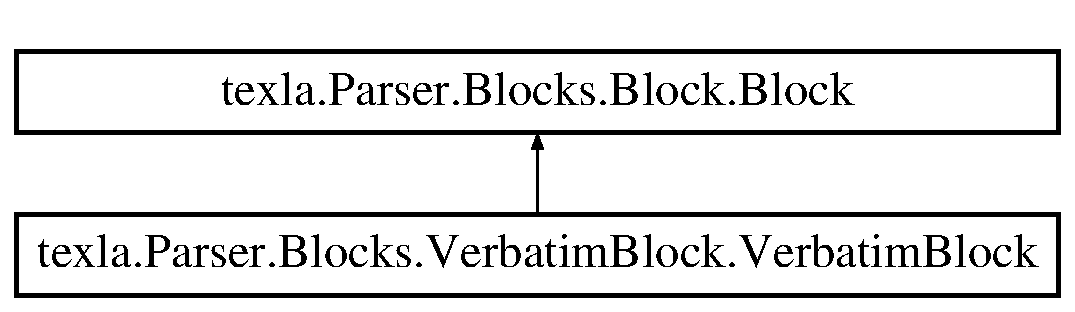
\includegraphics[height=2.000000cm]{classtexla_1_1Parser_1_1Blocks_1_1VerbatimBlock_1_1VerbatimBlock}
\end{center}
\end{figure}
\subsection*{Public Member Functions}
\begin{DoxyCompactItemize}
\item 
\hypertarget{classtexla_1_1Parser_1_1Blocks_1_1VerbatimBlock_1_1VerbatimBlock_a5945561c3968be307e655f7e8a5fbe17}{}\label{classtexla_1_1Parser_1_1Blocks_1_1VerbatimBlock_1_1VerbatimBlock_a5945561c3968be307e655f7e8a5fbe17} 
def {\bfseries \+\_\+\+\_\+init\+\_\+\+\_\+} (self, vtype, content, star, parent\+\_\+block)
\end{DoxyCompactItemize}
\subsection*{Static Public Member Functions}
\begin{DoxyCompactItemize}
\item 
\hypertarget{classtexla_1_1Parser_1_1Blocks_1_1VerbatimBlock_1_1VerbatimBlock_a7f397763341d83e66f26c22b65b6d0cc}{}\label{classtexla_1_1Parser_1_1Blocks_1_1VerbatimBlock_1_1VerbatimBlock_a7f397763341d83e66f26c22b65b6d0cc} 
def {\bfseries parse\+\_\+verbatim} (parser, tex, parent\+\_\+block, params)
\item 
\hypertarget{classtexla_1_1Parser_1_1Blocks_1_1VerbatimBlock_1_1VerbatimBlock_a2ff4ceb844ad660cf5304330d1e715e2}{}\label{classtexla_1_1Parser_1_1Blocks_1_1VerbatimBlock_1_1VerbatimBlock_a2ff4ceb844ad660cf5304330d1e715e2} 
def {\bfseries parse\+\_\+verb} (parser, tex, parent\+\_\+block, params)
\end{DoxyCompactItemize}
\subsection*{Additional Inherited Members}


\subsection{Detailed Description}
\begin{DoxyVerb}Starts an enviroment which will be typeset exactly
as you type it, carriage returns and all, usually in typewriter font\end{DoxyVerb}
 

The documentation for this class was generated from the following file\+:\begin{DoxyCompactItemize}
\item 
texla/\+Parser/\+Blocks/Verbatim\+Block.\+py\end{DoxyCompactItemize}

%--- End generated contents ---

% Index
\backmatter
\newpage
\phantomsection
\clearemptydoublepage
\addcontentsline{toc}{chapter}{Index}
\printindex

\end{document}
